%!TEX TS-program = pdflatex
%!TEX encoding = UTF-8 Unicode
%!TEX root = 2018-03-26-papa-vitres-de-son_libroA4.tex

\documentclass[a4paper,
		       titlepage,
               headinclude,
               footinclude,
               BCOR5mm,
               numbers=noenddot,
               cleardoublepage=empty,
               tablecaptionabove,
               twoside,
               openright,
               %openany
               ]{scrreprt}

\usepackage[T1]{fontenc}
\usepackage[utf8]{inputenc}

\usepackage[english,
            italian
            ]{babel}
            
\usepackage{amsmath,
		    amssymb}

\usepackage{indentfirst}

\usepackage[style=philosophy-modern,
            hyperref
            ]{biblatex}
            
\usepackage{chngpage}

\usepackage{calc}

\usepackage{listings}

\usepackage{graphicx}

\usepackage{subfig}

\usepackage{lipsum}

\usepackage{shapepar}

\usepackage{pifont}

\usepackage[eulerchapternumbers,
            subfig,
            beramono,
            eulermath,
            pdfspacing,
            listings,
            dottedtoc
            ]{classicthesis}

\usepackage{arsclassica}

% ********************************************************************
% Personal commands
% ******************************************************************** 
\newcommand{\myName}{Michele Papa}
\newcommand{\myTitle}{Vitres de Son}
\newcommand{\mySubTitle}{Come un rosone nel cuore di un tempio immenso}

\DeclareRobustCommand*{\clsname}[1]{{\normalfont\sffamily#1}}
\DeclareRobustCommand*{\pkgname}[1]{{\normalfont\sffamily#1}}
\DeclareRobustCommand*{\optname}[1]{{\normalfont\ttfamily#1}}
\DeclareRobustCommand*{\cmdname}[1]{\mbox{\lstinline[basicstyle=\normalsize\ttfamily]!\\#1!}}

\DeclareRobustCommand*{\classicthesis}{Classic\-Thesis}
\DeclareRobustCommand*{\arsclassica}{{\normalfont\sffamily ArsClassica}}


% ********************************************************************
% Hyper-references
% ******************************************************************** 
\newcommand{\mail}[1]{\href{mailto:#1}{\texttt{#1}}}


% ********************************************************************
% Graphics
% ********************************************************************
\graphicspath{{Graphics/}}


% ********************************************************************
% Code
% ********************************************************************
\definecolor{lightergray}{gray}{0.99}

\lstset{language=[LaTeX]Tex,
     keywordstyle=\color{RoyalBlue},
     basicstyle=\small\ttfamily,
     commentstyle=\color{Emerald}\ttfamily,
     stringstyle=\rmfamily,
     numberstyle=\scriptsize,
     showstringspaces=false,
     breaklines=true,
     frame=lines,
     backgroundcolor=\color{lightergray},
     flexiblecolumns=true,
     escapeinside={�*}{*�},
     firstnumber=last,
} 

\newcommand{\meta}[1]{$\langle${\normalfont\itshape#1}$\rangle$}

\lstset{	morekeywords=%
    {ProvidesPackage,RequirePackage,areaset,ifthenelse,%
     chapterNumber,undefined,boolean,DeclareRobustCommand,%
     spacedallcaps,textssc,MakeTextUppercase,lehead,%
     microtypesetup,textls,spacedlowsmallcaps,MakeTextLowercase,%
     sodef,allcapsspacing,lowsmallcapsspacing,thesection,%
     color,headmark,rohead,headfont,pnumfont,titleformat,%
     part,partname,thepart,chapter,thechapter,titlerule,%
     subsection,thesubsection,subsubsection,thesubsubsection,%
     paragraph,theparagraph,descriptionlabel,titlespacing,%
     formatchapter,textcolor,clearscrplain,rofoot,labelitemi,
     captionsetup,hypersetup}}

\lstnewenvironment{code}% 
   {\setkeys{lst}{columns=fullflexible,keepspaces=true}%
   \lstset{basicstyle=\small\ttfamily}}{}


% ********************************************************************
% Bibliography
% ******************************************************************** 
\bibliography{Bibliography}

\defbibheading{bibliography}{%
\cleardoublepage
\manualmark
\phantomsection
\addcontentsline{toc}{chapter}{\tocEntry{\bibname}}
\chapter*{\bibname\markboth{\spacedlowsmallcaps{\bibname}}
{\spacedlowsmallcaps{\bibname}}}}

\renewcommand*{\nameyeardelim}{\addcomma\space}

%-----------------------------------------------------------------------
%--------------------------------------------------- personalizzazioni -
%-----------------------------------------------------------------------

\usepackage{epigraph}

\usepackage{floatflt}

\usepackage{epsfig}

\usepackage{setspace}

%\linespread{1.1}

\usepackage{tikz}

\usepackage{color}

\usepackage{pdfpages} 

\usepackage{wrapfig} 

\usepackage{multirow}

\usepackage{booktabs}

\usepackage{tabularx}

%-----------------------------------------------------------------------
%----------------------------------------------------------- documento -
%-----------------------------------------------------------------------

\begin{document}

\pagenumbering{roman}

\pagestyle{plain}

%!TEX TS-program = pdflatex
%!TEX encoding = UTF-8 Unicode

%*******************************************************
% Titlepage
%*******************************************************

\begin{titlepage}
\pdfbookmark{Titlepage}{Titlepage}
\changetext{}{}{}{((\paperwidth  - \textwidth) / 2) - \oddsidemargin - \hoffset - 1in}{}
    \begin{center}

\begin{table}[htp]
\begin{center}
\begin{tabular}{rl}
\multirow{ 2}{*}{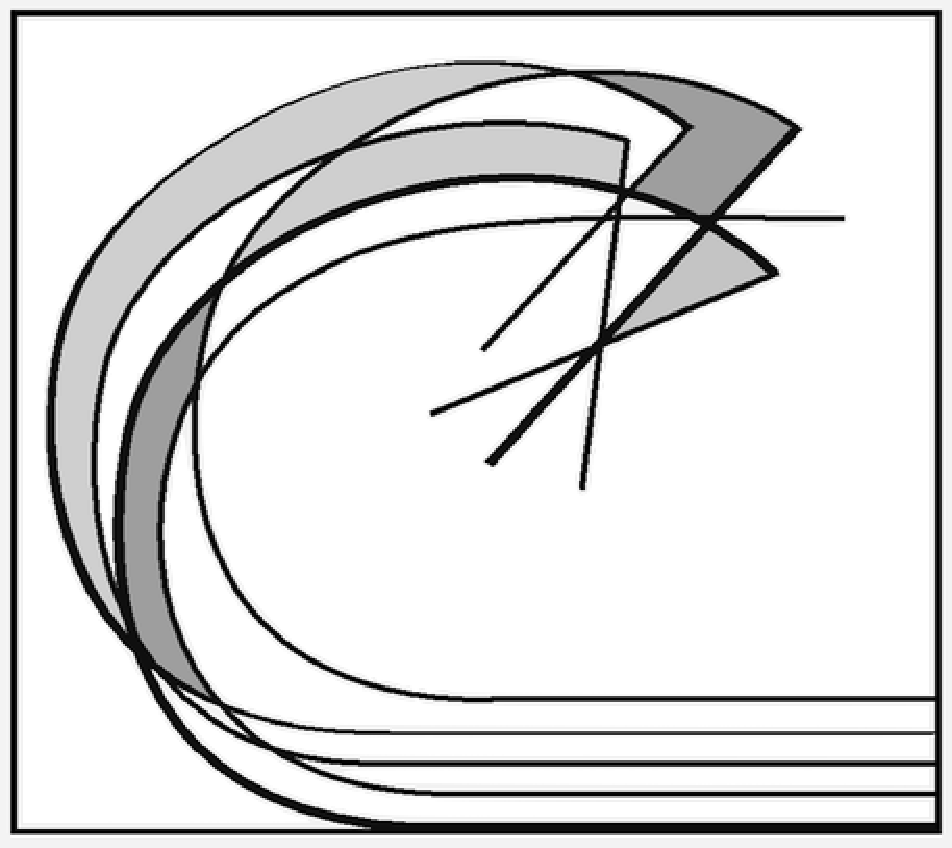
\includegraphics[scale=0.172]{Conservatorio.pdf}} & \LARGE \spacedlowsmallcaps{Conservatorio di Musica}\\ 
& \LARGE \spacedlowsmallcaps{S. Cecilia di Roma} \\ \cmidrule{2-2}
& \spacedlowsmallcaps{DIPARTIMENTO DI} \\
& \spacedlowsmallcaps{NUOVE TECNOLOGIE E LINGUAGGI MUSICALI} \\
& \spacedlowsmallcaps{SCUOLA DI MUSICA ELETTRONICA} \\
\end{tabular}
\end{center}
\label{default}
\end{table}%   

%        \LARGE \spacedlowsmallcaps{Conservatorio di Musica S. Cecilia di Roma}
%        
%        \bigskip
%        
%        \hrule
%        
%        \bigskip
%        
%        \large \spacedlowsmallcaps{DIPARTIMENTO DI NUOVE TECNOLOGIE E LINGUAGGI MUSICALI}
%        
%        \spacedlowsmallcaps{SCUOLA DI MUSICA ELETTRONICA}
        
		\vfill
        
        \spacedlowsmallcaps{CORSO DI DIPLOMA ACCADEMICO DI PRIMO LIVELLO IN}
                       
        \LARGE \spacedlowsmallcaps{MUSICA ELETTRONICA}

        \vfill 
        
        \begin{figure}[htbp]
\begin{center}
\includegraphics[width=.75\textwidth]{Rosone.pdf}
\end{center}
\end{figure}

        \LARGE {\color{Maroon}\spacedallcaps{\myTitle}}
        
        \large \mySubTitle 
        
        \vfill
        
        \normalsize Candidato: \\
        \Large \spacedlowsmallcaps{\myName}
        
        \normalsize Matricola: \\
        \Large \spacedlowsmallcaps{2945TR}
        
        \bigskip
        
        \normalsize Relatore: \\
        \Large \spacedlowsmallcaps{Michelangelo Lupone}

        \vfill ~ \vfill ~ \vfill
        
        \normalsize Anno Accademico: \\
        \Large \spacedlowsmallcaps{2016-2017}


%        
\includegraphics[width=0.7\textwidth]{TFZSuperEllisse} \\ \bigskip
                   

    \end{center}        

\end{titlepage} 

%\begin{figure}
%        \centering
%        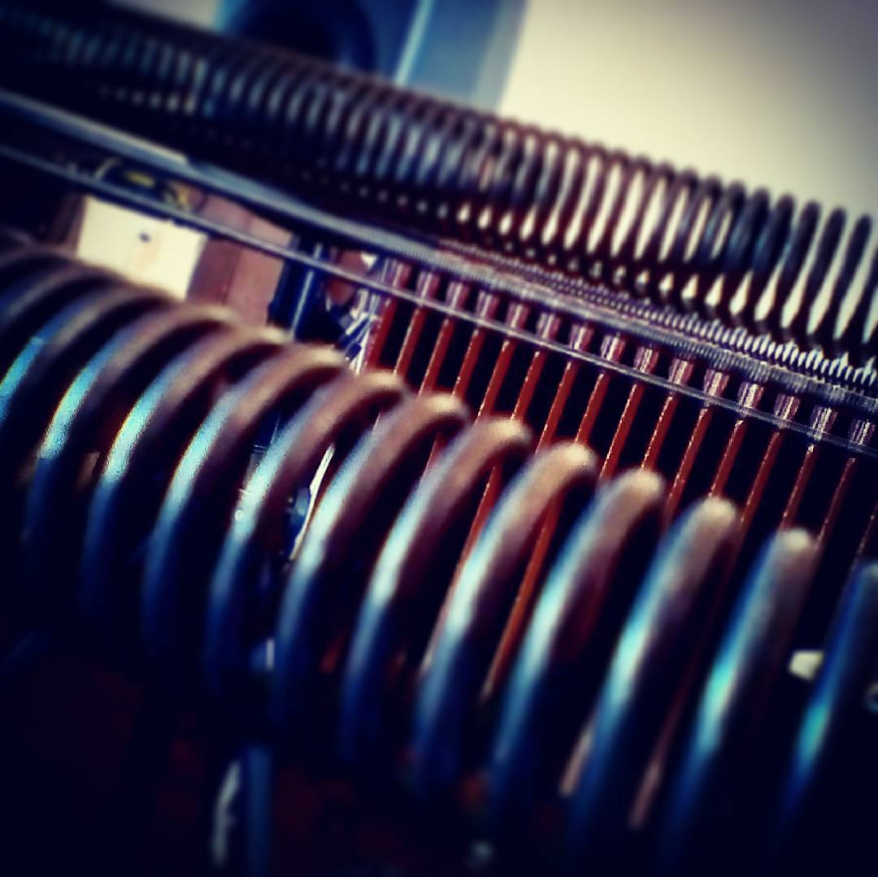
\includegraphics{spire.jpg}
%        \caption{Particolare dell'opera \textit{Sp.I.R.E.} - Foto scattata in Aula Bianchini, Conservatorio Santa Cecilia, Roma. 2018}
%   \end{figure}

\cleardoublepage

\thispagestyle{empty}

\includepdf[offset=-80 0,
		    scale=1.43,
		    pagecommand={
		    	\begin{tikzpicture}[
					remember picture,
					overlay]
		    	\node [xshift=10cm,yshift=1cm] at (current page.south west) {\color{white}{
			Particolare dell'opera \textit{Sp.I.R.E.} - Foto scattata in Aula Bianchini, Conservatorio Santa Cecilia, Roma. 2018}};
				\end{tikzpicture}}
		    ]{spire.pdf}

\cleardoublepage

%!TEX TS-program = pdflatex
%!TEX encoding = UTF-8 Unicode

%*******************************************************
% Dedica
%*******************************************************
\chapter*{Dedica}

\pdfbookmark{Dedica}{Dedica}

\textit{Dedicato a:}\\
Tutte le donne che ...\\
I miei genitori\\
Mia sorella\\
Giulia\\
i miei colleghi\\
il gruppo\\
Cesarina\\
Michelangelo e Massimo



\cleardoublepage

\pagestyle{scrheadings}

% !TEX TS-program = pdflatex
% !TEX root = ../ArsClassica.tex

%*******************************************************
% Contents
%*******************************************************
\phantomsection
\pdfbookmark{\contentsname}{tableofcontents}
\setcounter{tocdepth}{2}
\tableofcontents
\markboth{\spacedlowsmallcaps{\contentsname}}{\spacedlowsmallcaps{\contentsname}} 

\cleardoublepage

\singlespacing
\linespread{1.1}
%\doublespacing

\pagenumbering{roman}

%!TEX TS-program = pdflatex
%!TEX encoding = UTF-8 Unicode
%!TEX root = ../2018-03-26-papa-vitres-de-son.tex

%*******************************************************
% Introduzione
%*******************************************************

\pdfbookmark{Introduzione}{Introduzione}

Ogni creazione artistica è legata imprescindibilmente sia alla carriera accademica che alla storia personale di chi la scrive. \\
Nel corso della stesura di questa tesi, ho cercato di esprimere il mio processo compositivo e creativo. La forma del testo, per una resa più diretta e scorrevole, è in forma romanzata, è una storia. Cercando in qualche modo di sfuggire da una semplice compilazione di liste sulle tecniche e sui materiali sonori utilizzati. \\
Questa composizione è più un sentiero da intraprendere ed è forse questo il lavoro che un compositore elettroacustico fa giornalmente: non la sola scrittura notazionale e simbolica, ma una continua ricerca di fenomeni che incarnino il proprio vissuto e nel quale un artista può identificarsi, facendoli suoi e riportandoli in musica, creando una propria identità artistica e formale. Come scrisse Kandisky nell'introduzione di \textit{Punto e linea nel piano}: 
\begin{small}
\begin{quotation}
\textit{Di ogni fenomeno si può fare esperienza in due modi. \\ Questi due modi non sono arbitrari ma connessi ai fenomeni -  essi vengono derivati dalla natura dei fenomeni, da due proprietà degli stessi: \\ 
\centerline{esterno - interno\footnote{Wassily Kandisky \textit{Punto e linea nel piano}, Adelphi Edizioni, Roma, 1968}.}}
\end{quotation}
\end{small}


Muovere \textit{interna}mente le corde della propria coscienza e delle proprie esperienze, provando a far vibrare ogni suggestione verso qualcosa di nuovo. Per "qualcosa di nuovo" non intendo un oggetto o una scrittura mai letta o vista prima. Il nuovo, penso, sia semplicemente l'unione di tecniche e di procedimenti fisici che per la prima volta subiscono quella successione di eventi nel tempo. Il tempo crea il nuovo nelle svariate possibilità che la vita ci propone: verso un \textit{esterno} dove abbiamo la possibilità di essere semplici ascoltatori o fautori dei cambiamenti che avvengono in tale realtà. 


\pagenumbering{arabic}

% !TEX TS-program = pdflatex
% !TEX encoding = UTF-8 Unicode
% !TEX root = ../ArsClassica.tex

%************************************************
\chapter{Sinossi}
\label{chp:Sinossi}
%************************************************

\textit{Vitres de Son - Come un rosone nel cuore di un tempio immenso} non è solo una composizione legata alla creazione e alla ricerca su un nuovo \textit{oggetto sonoro}, ma fa parte di un percorso compositivo e creativo che dura ormai da quattro anni. \\
Il titolo e il sottotitolo dell'opera sono rispettivamente il titolo e un verso di due poesie del drammaturgo, poeta e attore Antonin Artaud: \textit{Vitres de Son} e \textit{In Sogno}. Entrambe le poesie sono presenti in \textit{Poesie della crudeltà}\footnote{Antonin Artaud, \textit{Poesie della crudeltà} (a cura di P. Di Palmo), Stampa alternativa, Roma 2002, a cura di P. Di Palmo. Pubblicata per la prima volta nel 1925 \\}. \\
Artaud era artista ai margini, esponente del movimento surrealista e molto discusso dalla critica per le sue idee estremiste riguardanti il teatro, la messa in scena  e la modalità di diffusione della sua arte:
\begin{small}
\begin{quotation}
\textit{Nell'epoca di confusione in cui viviamo, epoca colma di bestemmie e delle fosforescenze di un rinnegamento infinito, in cui tutti i valori sia artistici che morali sembrano sprofondare in un abisso senza altro esempio in nessun epoca dello spirito, ho avuto la debolezza di credere che avrei potuto fare un teatro, che avrei potuto almeno avviare il tentativo di ridare vita al valore universalmente disprezzato del teatro, ma la stupidità di alcuni, la malafede e la spregevole canaglieria di altri me ne hanno distolto per sempre. } [...] \footnote{Antonin Artaud, \textit{Il teatro e il suo doppio}, Einaudi Autore, Roma 1968 \\}
\end{quotation}
\end{small}
L'artista spinge verso una critica sociale che lo porterà ai margini della società e nella quale mi rispecchio. Inoltre, la figura del drammaturgo si può accostare a quella dei \textit{clerici vagantes}\footnote{Furono così chiamati per tutto il sec. XII e il XIII quei poeti, che, vivendo al margine della chiesa, vagavano per le università, le città e le corti, spesso confusi con i giullari, di cui condividevano la vita errabonda e l'indole artistica. [...] \\ \textit{Enciclopedia Treccani} Edizione 2018. \\}. Sia Artaud che i clierici erano, infatti, personaggi solitari, irrequieti, artisti vaganti che risentirono quel potente risveglio intellettuale e politico della loro epoca (in entrambe le epoche), rispecchiandone le condizioni sociali ma soprattutto la fisionomia morale. L'artista è sempre stato un personaggio ai margini e soprattuto Artaud ha ricevuto non poche cure psichiatriche dopo essere arrivato a deliri tali da fermarlo anche nella sua produzione artistica. Per fortuna, le poesie utilizzate per la composizione del mio lavoro, sono legate al primo periodo artistico, quello giovanile, dove ancora riesce ad esprimere un proprio universo immaginifico. Il suo è un paesaggio fatto di personaggi e suoni, potrei azzardare quasi un \textit{paesaggio sonoro}, alla maniera di Schafer, dove ogni cosa, ogni suono, può diventare personaggio.
\begin{quotation}
[...] \\
come un rosone nel cuore di un tempio immenso. \\
E là ascolteremo la cadenza immortale \\
delle linee e dei corpi ritmati \\
e di gotiche balaustre profumate \\
dalla dolcezza dei corpi amati \\
dagli uomini con grandi anime cadenzate, \\
\centerline{dai poeti profumati\footnote{Antonin Artaud, \textit{In Sogno} in Poesie della crudeltà \\}.}
\end{quotation}

Ecco, qui entra in gioco la fase di analisi e costruzione compositiva: l'unione di una visione - all'esterno - ascoltando, ad esempio, delle risonanze create da dita sui del rosone nel cuore del tempio immenso: riecheggiano - all'interno \footnote{qui faccio riferimento a \textit{Punto e linea nel piano} di Kandisky \\}- di un ambiente vuoto.
Al margine delle balaustre, assieme ad Artaud e i clerici vagantes, osserviamo i cambiamenti che avvengono sul linguaggio e sulla sua forma, sull'ambiente. \\
\begin{quotation}
\textbf{Vitres de Son} \\
Vitres de son où virent les astres \\
verres où cuisent les cerveaux \\
le ciel fourmillant d'impudeurs \\
dévore la nudité des astres. \\ \\ 
Un lait bizarre et véhément \\
fourmille au fond du firmament \\
un escargot monte et dérange \\
la placidité des nuages. \\ \\ 
Délices et rages, le ciel entier \\
lance sur nous comme un nuage \\
un tourbillon d'ailes sauvages \\
torrentielles d'obscénités\footnote{Artaud, \textit{Vitres de Son} in Poesie della crudeltà \\}. \\
\end{quotation}
I \textit{Vetri di suono} diffondono un materiale acustico fascinoso sia nella forma di diffusione elettroacustica che nella tipologia del gesto: mentre l'eccitazione delle armoniche e la componente elettronica, ci spingono verso l'alto, la vibrazione delle sub-armoniche di grandi molle \footnote{vedi cap. 2 \\} ci terrà con i piedi ben saldi al pavimento antistante alla cattedrale, astrazione immaginifica della sala da concerto. \\
Davanti a questo universo fatto di paesaggi e personaggi sonori, entra in causa la composizione. Il processo compositivo legato alle immagini e al ritmo dei versi di Artaud sarà il fulcro dominante dell'andamento formale di \textit{Vitres de Son - Come un rosone nel cuore di un tempio immenso}.


% !TEX TS-program = pdflatex
% !TEX encoding = UTF-8 Unicode

%************************************************
\chapter{L'opera Sp.I.R.E}
\label{chp:L'opera Sp.I.R.E}
%************************************************

	\begin{flushright}
		\textit{[...] bello come la retrattilità degli artigli degli uccelli rapaci; o ancora, come l'incertezza dei movimenti muscolari nelle pieghe delle parti molli della regione cervicale posteriore; [...] e soprattutto, come l'incontro fortuito su un tavolo di dissezione di una macchina da cucire e di un ombrello!
		Isidore Lucien Ducasse}
	\end{flushright}

Tutto ebbe inizio nel luglio del 2017.

Nel corso della manifestazione \textit{ArteScienza 2017} tenutasi al Goethe Institute, venne eseguita una composizione di Pierre Jodlowski: \textit{Ombra della Mente}, ispirata ad alcuni scritti di Alda Merini. Il lavoro del compositore francese era diviso tra una parte teatrale recitata e una parte musicale, entrambe eseguite da una clarinettista e da una soprano. La fusione tra momenti prettamente teatrali e parti musicali ebbero un effetto tagliente sulla mia produzione musicale. Ogni intervento recitante era contrappuntato da rumori prodotti tramite lo strofinio di una matita su un foglio di carta e la frizione di una piccola molla presente nella meccanica della lampada di scena. Il tutto era elaborato in live electronics. L'effetto della molla sfregata e amplificata da un microfono a contatto, mi fece riaffiorare alla mente molti concerti di musica underground seguiti in passato (l'utilizzo delle molle, oltre ad appartenere all'universo della musica colta è stato abusato in ambienti musicali \textit{noise}\footnote{genere che utilizza il rumore come base principale per creare delle composizioni} e di musica cosiddetta "industriale" (chiamata così, proprio per sottolineare l'utilizzo di materiale di scarto di industrie e fabbriche).

\begin{small}
\begin{quotation}
[...] still the noise in the mind: that's it's the first task - then everything else will follow in time\footnote{R. Murray Schafer, \textit{The tuning of the world}, Alfred A. Knopf, New York 1977 \\}.
\end{quotation}
\end{small}

Andando avanti negli studi notai che, già negli anni '50 del Novecento, John Cage cercò di far percepire, tramite l'amplificazione con elettromagneti e microfoni a contatti, i suoni non udibili\footnote{qui faccio riferimento a \textit{Cartridge Music}}. Durante il corso di \textit{Interpretazione del repertorio della musica elettroacustica} del Mº Giuseppe Silvi ripercorremmo tutto lo scenario cagiano e iniziai, così, ad interessarmi in modo più accurato all'universo delle molle e alle loro particolarità timbriche.

\begin{small}
\begin{quotation}
Si può dire che la musica moderna in generale è stata la storia della liberazione della dissonanza, così la nuova musica è parte del tentativo di liberare tutti i suoni udibili dalle limitazioni del pregiudizio musicale.
Un singolo suono in sé non è né musicale né non musicale; è semplicemente suono. [...]

La musica mi sembrava ora l'organizzazione del suono, l'organizzazione di qualunque suono ottenuto con qualunque mezzo\footnote{John Cage, \textit{Confessioni di un compositore} in AA.VV. (a cura di G. Bonomo e G. Furghieri), \textit{Riga n. 15} - John Cage, Milano, Marcos y Marcos, Milano 1998}.
\end{quotation}
\end{small}

Dalle parole di Cage emerge una sostanziale verità, ovvero, tocca al compositore trasformare un suono in qualcosa di musicale, legando ad un andamento formale adeguato. 

Iniziai così le ricerche sia sui materiali e gli oggetti sonori che su forme musicali vicine allo scenario contemporaneo. Fortuito fu il lavoro assieme al Mº Michelangelo Lupone al Centro di Ricerche Musicali (CRM) sito in Roma. Per tutta l'estate del 2017 gli feci da assistente per la creazione di un'installazione ideata in collaborazione con l'artista Licia Galizia. L'opera in questione era la scenografia interattiva dello spettacolo coreutico \textit{Corpus 2.0}. Il lavoro consisteva nell'applicare all'interno dell'installazione, vari diffusori e piezoelettrici che servivano rispettivamente per la diffusione sonora e l'interazione con i danzatori. L'utilizzo di specifici altoparlanti e il controllo di parametri tramite il tocco, mi fece avvicinare ad un mondo a me limitrofo ma ancora in parte sconosciuto: quello dell'interazione tra uomo e macchina.

%************************************************

\section{Necessità di uno strumento dedicato}

\begin{small}
\begin{quotation}
Lo strumento musicale è il risultato di un insieme complesso di condizioni culturali.

Le sue caratteristiche tecnologiche e la sua \textit{structura} di oggetto composto, devono consentire la rappresentazione di un determinato linguaggio musicale, caratterizzato da aspetti estetici, espressivi e stilistici che implicano una prassi esecutiva consolidata, o almeno condivisa in un determinato contesto\footnote{Silvia Lanzalone Strumenti aumentati in Acustica UTET}.
\end{quotation}
\end{small}

La creazione di uno strumento musicale, quindi, comportava molte problematiche soprattutto a livello stilistico e di concetto. 

\begin{small}
\begin{quotation}
La ricerca di una definizione ontologica della musica è quindi strettamente connessa alla definizione dei confini tra un semplice oggetto che produce suono e uno strumento musicale, la cui prerogativa non può prescindere dal riconoscimento di un suo ruolo funzionale o simbolico in una data società\footnote{\textit{ibidem}}.
\end{quotation}
\end{small}

La linea di confine tra uno strumento musicale e un oggetto che produce suono è strettamente legata al suo utilizzo. Basandomi su queste nozioni, mi presi del tempo per far sedimentare in me delle nuove idee. Le giornate di lavoro al CRM diventarono fonte di suggestioni sull'utilizzo di oggetti risonanti e sulle loro capacità timbriche. Ogni oggetto sonoro diventò frutto di studio, anche minimo a volte, per via dei tempi brevi dati dalle consegne. Questo fu l'universo sonoro al quale mi aggrappai per la fascinazione che suscitava in me.

Giorno per giorno si andava a materializzare un'idea sempre più nitida, fino al giorno del mio esame del III anno di composizione elettroacustica.

Un esercizio, un brano, un piccolo studio sulle armoniche del pianoforte. La composizione partiva dalla trasformazione di un gesto sonoro: il pedale di risonanza in \textit{\textbf{fff}} seguito da cellule sonore inarmoniche composte da cluster e piccole volatine. I Gesti venivano elaborati tramite tre convoluzioni. Ogni convolutore apparteneva ad un universo sonoro a sé:

\begin{itemize}
\item{la prima convoluzione era la stessa cassa di risonanza del pianoforte eccitata dal pedale di risonanza calcato in \textit{\textbf{fff}};}
\item{la seconda convoluzione era creata registrando la molla della stessa lampada da tavolo utilizzata da Pierre Jodlowski;}
\item{la terza convoluzione era un'eccitazione del manico di una chitarra elettrica su un amplificatore a transistor.}
\end{itemize}

%\begin{floatingfigure}{10cm}
%\mbox{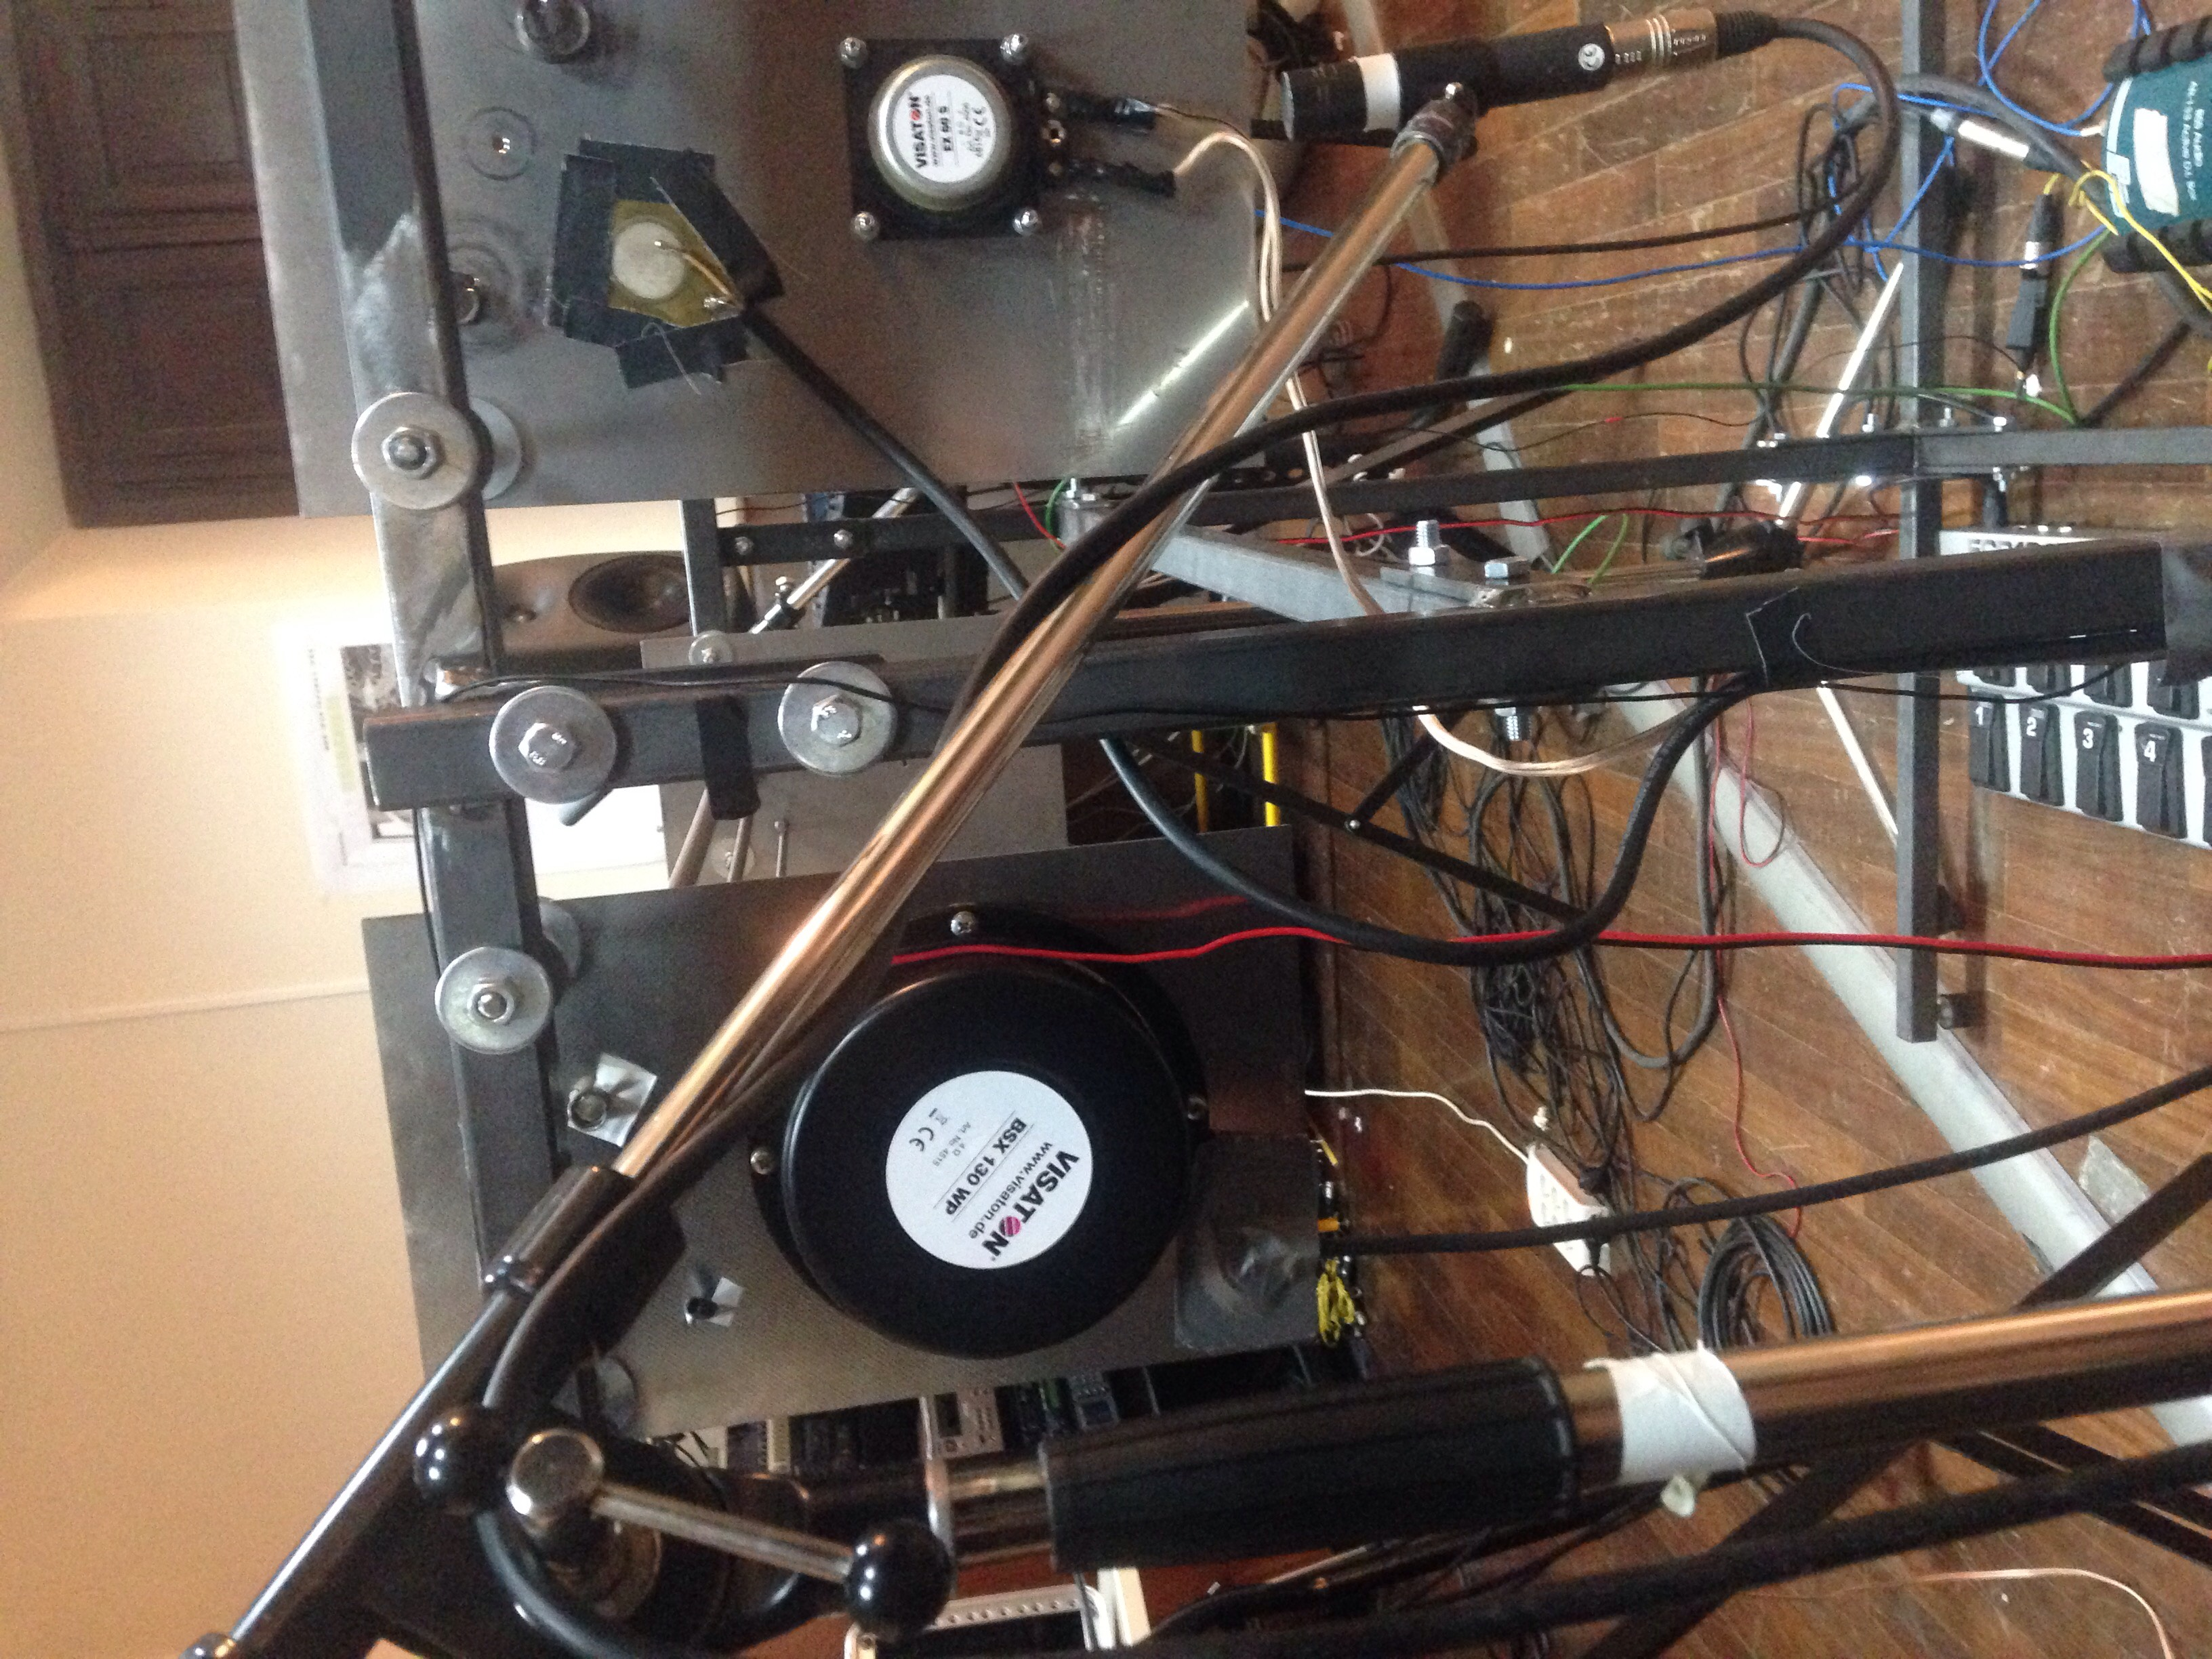
\epsfig{file=Spire1.jpg,width=8cm}}
%\small{\caption{\textit{particolare attuatori}}}
%\end{floatingfigure}
%

I risultati delle convoluzioni erano affascinanti, ma non mi soddisfacevano,  era come se volessi creare un convolutore che potesse essere, in qualche modo, anche un gesto scenico. Da qui alla creazione del mio iper-strumento, il passo fu breve. Riuscii finalmente ad avere del tempo per finire di progettare il basamento. Mi confrontai con un mio collega, Leonardo Mammozzetti, riguardo le specifiche tecniche di costruzione, ovvero materiali, agganci e tempi di costruzione. Mammozzetti provvedette a trovare i metalli per la costruzione e nel giro di un mese il basamento era pronto.

\begin{figure}[htbp]
\begin{center}
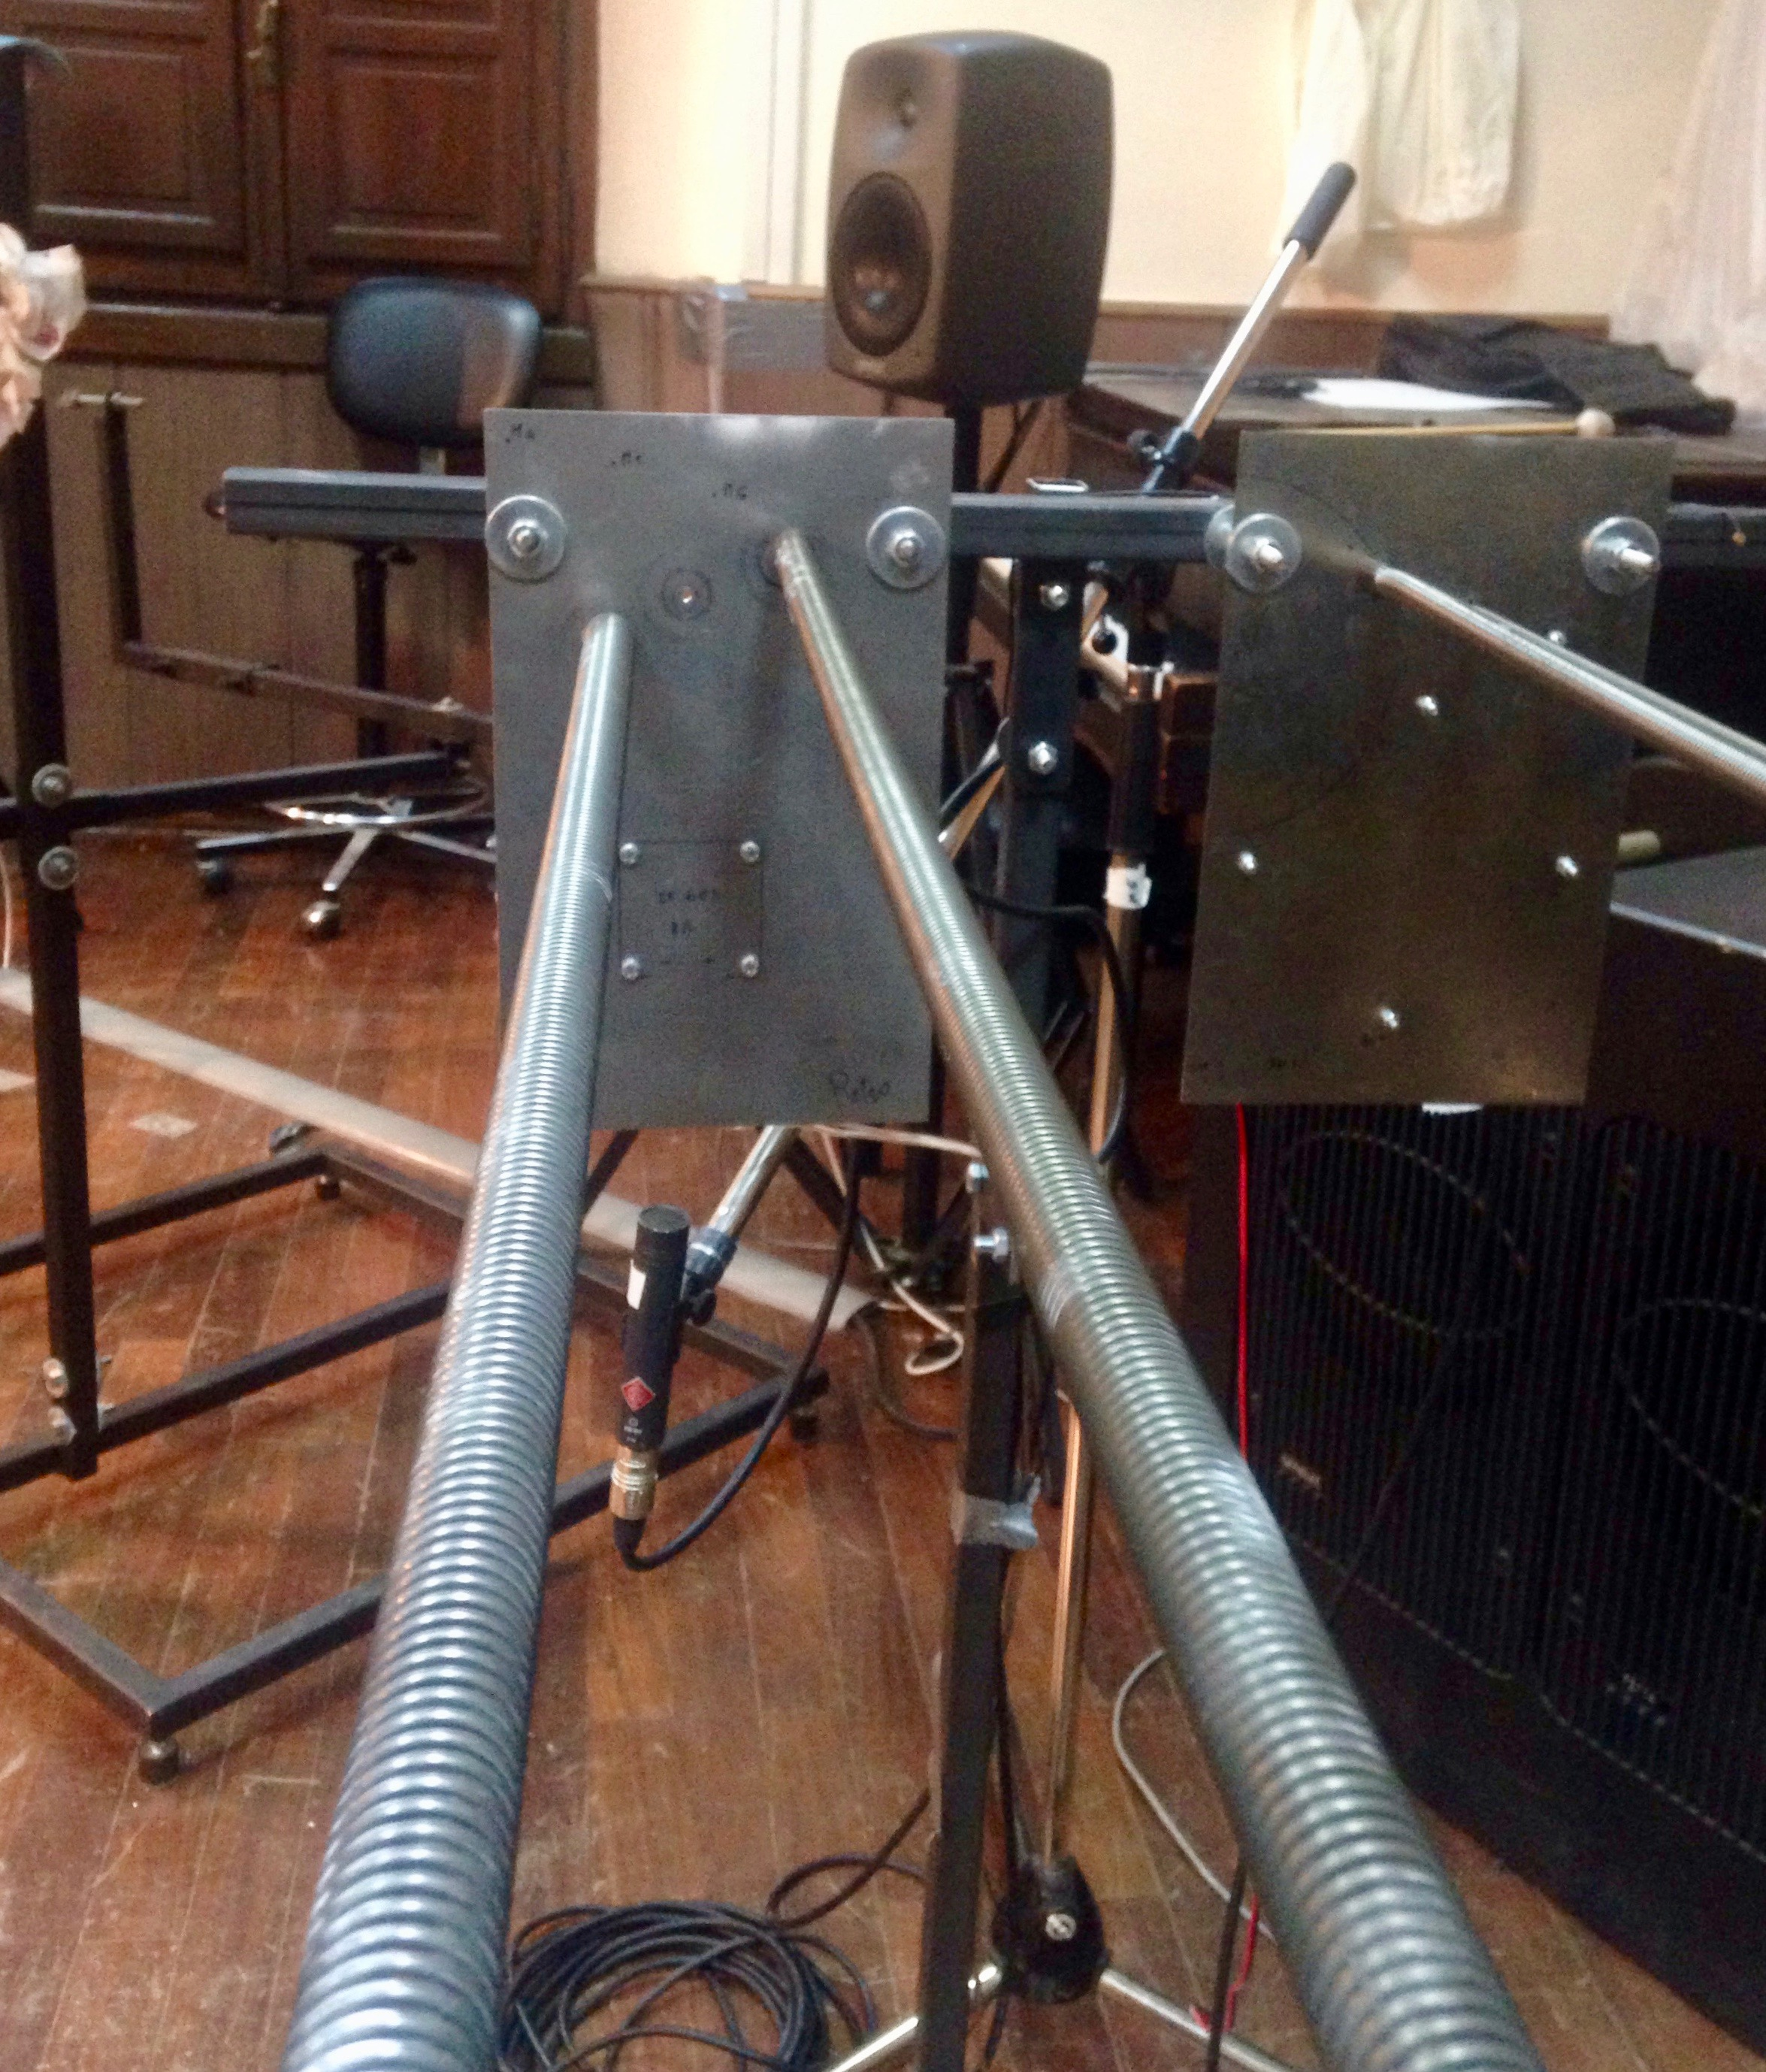
\includegraphics[width=.99\textwidth]{Spire2cc.jpg}
\caption{\textit{Sp.I.R.E.}, particolare della sezione più grave (Molla 5-4)}
\label{default}
\end{center}
\end{figure}

Lentamente l'oggetto prendeva forma, il CRM mi fornì le lastre mancanti e il \textit{Mollificio Ciullo} \footnote{https://www.mollificiociullo.com} mi indirizzò nella scelta delle molle. Potei finalmente vedere, ma soprattutto sentire se tutte le mie idee portavano a qualcosa di reale. La svolta decisiva la ebbi durante il montaggio delle lastre, perché decisi di aggiungere una variante elettroacustica: degli attuatori. Gli attuatori (diffusori capaci di far risuonare il materiale sul quale vengono collocati) furono il tassello mancante. Come scrive Silvia Lanzalone in un suo saggio:

\begin{quotation}
\textit{La catena elettroacustica, nonostante il notevole perfezionamento tecnologico degli ultimi decenni verso l'accuratezza della riproduzione sonora, conferisce ancora al suono una trasformazione finale dovuta alla natura elettromeccanica dei suoi componenti, imponendovi dunque una deformazione che la rende decorrelata dal segnale che trasmette, nonché estranea ad esso dal punto di vista della sua identificazione percettiva nello spazio destinato alla sua diffusione}\footnote{Silvia Lanzalone \textit{Strumenti aumentati} in \textit{Acustica} UTET}.
\end{quotation}

Spesso, quasi sempre, il suono elettronico risulta svincolato dal suono acustico. L'aggiunta degli attuatori sulle lastre, fu, perciò, il passo vincente per ovviare a tale problematica. Agire come se stessi "aumentando" uno strumento acustico è stato il pensiero principale, anche se ancora trattavo l'opera come un \textit{oggetto sonoro}. Nelle prove, convogliai tutti i contributi elettronici (dalle elaborazioni alla sintesi) direttamente nei quattro attuatori,  trasformando così il mio oggetto sonoro in un vero e proprio \textit{strumento elettroacustico}: possibilità di rilascio "acustico" del suono e quindi interazione tra elementi acustici ed elettronici. 

Era nato lo \textit{Sp.I.R.E.}

%\begin{floatingfigure}{10cm}
%\mbox{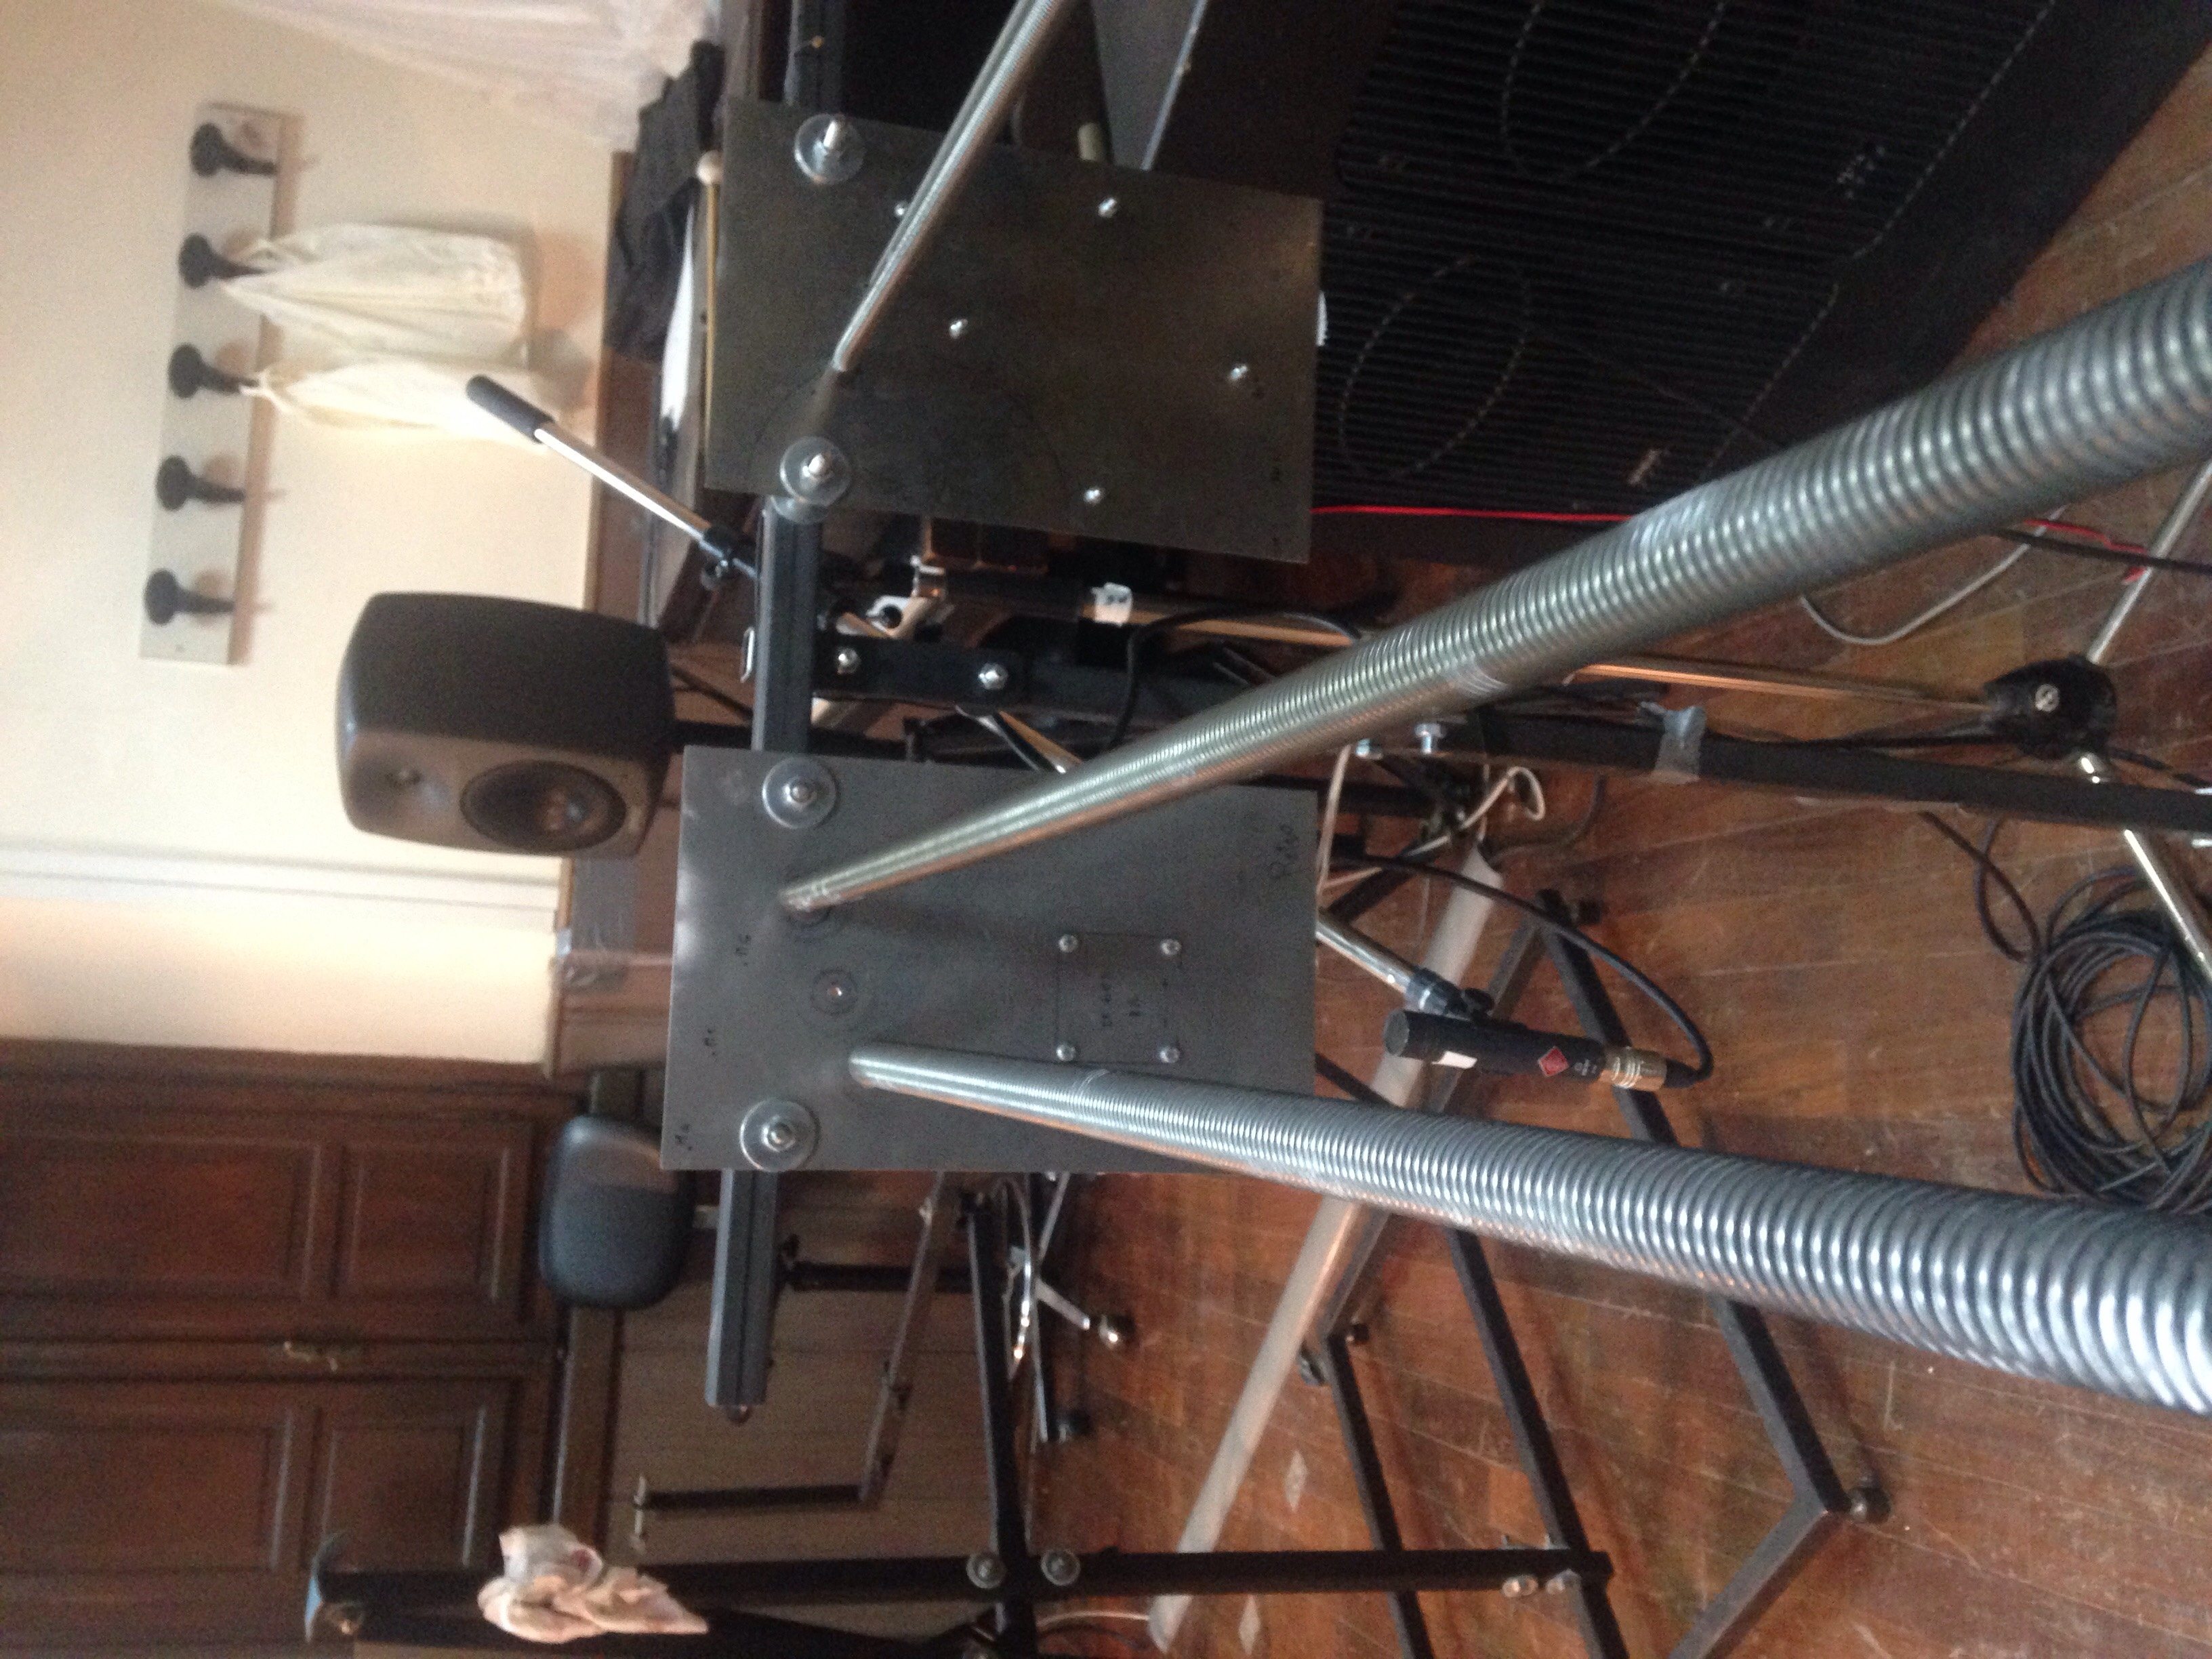
\epsfig{file=Spire2.jpg,width=8cm}}
%\small{\caption{\textit{particolare molle}}}
%\end{floatingfigure}



\textit{Sp.I.R.E.}, acronimo di \textit{Springs Installation Regulated \& Electrified}, fa riferimento alla fisicità del materiale che compone lo strumento. Ogni molla (\textit{spring}), infatti, è formata da \textit{spire} e il loro numero rende possibile, a seconda del materiale con il quale vengono eccitate, l'attivazione di armoniche e/o sub-armoniche. La parola \textit{electrified} indica la componente elettroacustica.

%\begin{floatingfigure}{10cm}
%\mbox{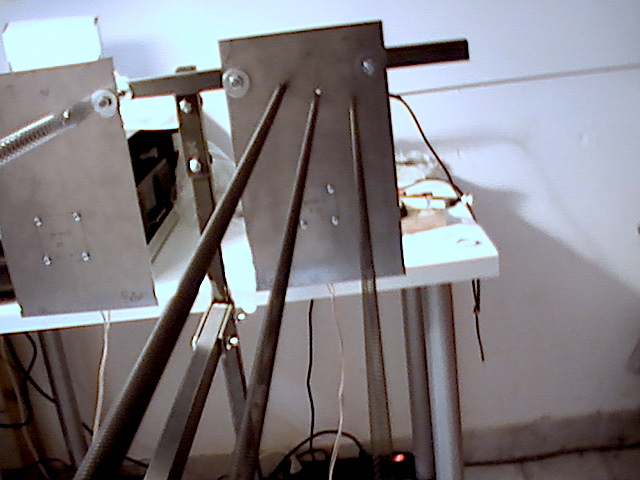
\epsfig{file=Prototipo2.jpg,width=8cm}}
%\small{\caption{\textit{particolare}}}
%\end{floatingfigure}

\begin{figure}[htbp]
\begin{center}
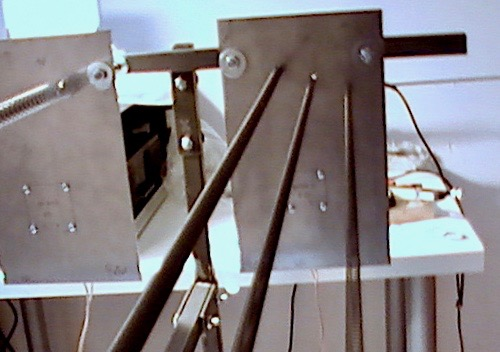
\includegraphics[width=.99\textwidth]{Prototipo2cc.jpg}
\caption{\textit{Sp.I.R.E.}, particolare della sezione più acuta (Molla 3-2-1)}
\label{default}
\end{center}
\end{figure}

Questo esperimento è connesso allo studio di nuove identità formali relative alla natura dello strumento e alla realtà installativa dell'opera, che induce chi guarda e ascolta, a toccare la materia e ad incuriosirsi verso materiali come molle e placche di metallo, utilizzate per scopi lontani dall'utilizzo che se ne fa ogni giorno.

%************************************************

\section{Intenzioni espressive}

\epigraph{\textbf{spirare} v. intr. e tr. [lat. spirare «soffiare»; respirare; emanare»]"}
{\textit{Enciclopedia Treccani}}
La prima intenzione espressiva fu la creazione di uno strumento che avesse in sé le qualità del reverbero a molle e del reverbero a piastra. Il risultato fu esaltante: le molle sfregate con dita o archetti generavano un ambiente sonoro che le piastre amplificavano e modificavano, generando una coda piena di una propria identità timbrica.

Sp.i.r.e. è un progetto ambizioso che vuole, tra le altre cose, reinterpretare ed ampliare la visione di John Cage in Cartridge Music. La ricerca è basata, appunto, sul riuscire a rendere percepibili i suoni non udibili prodotti dallo strofinio delle molle o delle placche. Può essere considerato a tutti gli effetti uno strumento musicale, perché legato sia al mondo dei cordofoni che all'universo degli idiofoni (nel corso della performance verranno utilizzati sia archetti che battenti per percussioni).

\begin{figure}[htbp]
\begin{center}
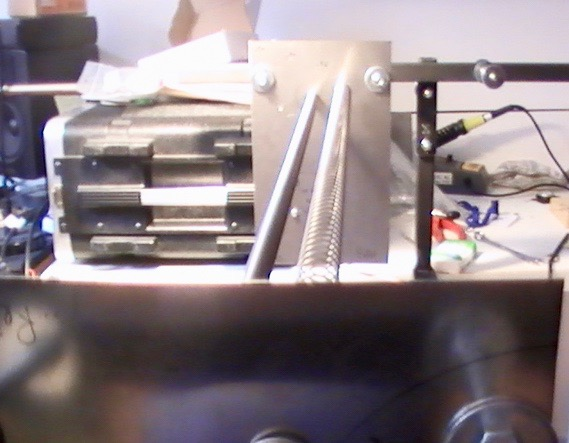
\includegraphics[width=.99\textwidth]{Prototipo3cc.jpg}
\caption{Foto scattata durante lavorazioni su Sp.I.R.E.}
\label{default}
\end{center}
\end{figure}

%************************************************

\section{Intenzioni estetiche}
Il progetto rappresenta il legame che c'è tra noi e il mondo che ci circonda: tutt'uno con la metropoli e con i fenomeni all'interno e all'esterno di essa\footnote{qui faccio riferimento di nuovo al concetto di fenomeno di Kandisky}.

Questa è l'identità di Sp.i.r.e., finalmente si tocca con mano la parte nascosta della materia, il lato più profondo di quello che vediamo attorno a noi. In unione ai suoni non udibili e all'invisibile, si scorge un richiamo verso una visione immaginifica che porta fino a dentro la nostra anatomia. Come se le spire della molla possono essere ricondotte ai ripiegamenti dell'intestino; come se, all'eccitazione di una molla, si riconduca la possibilità di produrre delle sub-armoniche e, in qualche modo, di avvicinarsi alle vibrazioni interne dell'anatomia umana.

La meccanica, l'elettronica e i suoni analogici, rendono possibile la creazione di un mondo nuovo. Vengono a formarsi più dimensioni d'ascolto e più dimensioni tattili, causate dalle diverse risposte d'eccitazioni del materiale. A questa dimensione d'ascolto si unisce la ripresa microfonica, che, nel caso di \textit{Vitres de Son}, sarà omnidirezionale e renderà possibile la riproduzione di tutto il panorama d'ascolto. Sp.i.r.e. \textit{respira} ed \textit{emana} il segnale elettroacustico in almeno due dimensioni d'ascolto:
\begin{enumerate}
\item{\textit{Analogica}, la risposta del materiale relativa ai suoni sintetici e al tocco umano}
\item{\textit{Elettrica ed elettronica}, che prende vita grazie ai suoni di sintesi diffusi dagli attuatori}
\end{enumerate}

L'insieme dei due fattori ha dato vita ad uno strumento che ingloba in sé, sia caratteristiche installative che performative. Una strana creature capace di suonare sia amplificata che in acustico grazie agli attuatori e al connubio fra placche e molle. La struttura è tutta \textit{suono}. Tendo a sottolineare che questo è ancora un primo prototipo e non mi fermerò prima di aver raggiunto determinati obbiettivi costruttivi e/o miglioramenti da applicare a breve sullo strumento. Come scrive Cage:

\begin{small}
\begin{quotation}
Decisi così di lavorare con qualunque strumento di produzione avessi incontrato e di tenere sempre un orecchio a terra, in cerca di un suono nuovo\footnote{John Cage, \textit{Confessioni di un compositore}}.
\end{quotation}
\end{small}

\clearpage

%************************************************

\section{Analisi spettrale}

Di seguito, l'analisi spettrale e lo spettrogramma della risposta all'eccitazione di ogni singola molla. 

\begin{figure}[htbp]
\begin{center}
\includegraphics[width=.99\textwidth]{MOLLA1.jpg}
\caption{Eccitazione \textit{Molla 5} tramite battente in legno.}
\label{default}
\end{center}
\end{figure}

Sottolineo che l'eccitazione della molla è provocata colpendo al centro della molla. 
Negli studi fatti in questi mesi ho registrato un decadimento differente a seconda del battente utilizzato.
Si può notare come, sia l'attacco, che l'eccitazione delle armoniche è maggiore con questo battente. Ogni molla è soggetta ad un inviluppo e a un decadimento differente. Il decadimento è lungo circa 10 secondi, mentre l'attacco è molto veloce: tra 0,4 e 0,6 millisecondi. 
L'ultimo grafico rappresenta l'eccitazione di una molla con un battente in metallo (fig. 5.d). 

\begin{figure}[htbp]
\begin{center}
\includegraphics[width=.99\textwidth]{MOLLA2.jpg}
\caption{Eccitazione \textit{Molla 4} tramite battente in legno.}
\label{default}
\end{center}
\end{figure}

\begin{figure}[htbp]
\begin{center}
\includegraphics[width=.99\textwidth]{MOLLA3.jpg}
\caption{Eccitazione \textit{Molla 3} tramite battente in legno.}
\label{default}
\end{center}
\end{figure}

\begin{figure}[htbp]
\begin{center}
\includegraphics[width=.99\textwidth]{MOLLA4.jpg}
\caption{Eccitazione \textit{Molla 2} tramite battente in legno.}
\label{default}
\end{center}
\end{figure}
%
%
%
\begin{figure}[htbp]
\begin{center}
\includegraphics[width=.99\textwidth]{MOLLA5.jpg}
\caption{Eccitazione \textit{Molla 5} tramite battente in metallo.}
\label{default}
\end{center}
\end{figure}

%\begin{figure}
%\centering
%\subfloat[][\emph{Eccitazione \textit{Molla 2} tramite battente in legno.}]
   %{\includegraphics[width=.75\textwidth]{MOLLA2.jpg}} \\
%\subfloat[][\emph{Eccitazione \textit{Molla 3} tramite battente in legno.}]
   %{\includegraphics[width=.75\textwidth]{MOLLA3.jpg}} \\
%\subfloat[][\emph{Eccitazione \textit{Molla 4} tramite battente in legno.}]
   %{\includegraphics[width=.75\textwidth]{MOLLA4.jpg}} \\
%\subfloat[][\emph{Eccitazione \textit{Molla 5} tramite battente in metallo.}]
   %{\includegraphics[width=.75\textwidth]{MOLLA5.jpg}}
%\caption{analisi spettrale all'eccitazione di ogni singola molla}
%\label{fig:subfig}
%\end{figure}


% !TEX TS-program = pdflatex
% !TEX encoding = UTF-8 Unicode

%************************************************
\chapter{La Performance}
\label{chp:La Performance}
%************************************************

\begin{quotation}
Since music began to be notated, clearer distinctions between the work and its performance, and between the composer and performer, have emerged, representing multifarious views of the role of the performer.\footnote{Tanja Orning \textit{Pression} (a performance study) Norwegian Academy of MusicMusic Performance Research Copyright © 2012 Royal Northern College of Music Vol. 5}
\end{quotation}

Introduco questo paragrafo con una citazione estrapolata da un articolo scritto da Tanja Orning su \textit{Pression} di Helmut Lachenmann. La semplicità con la quale il compositore è riuscito a trasformare il gesto in scrittura è di grande interesse. infatti, è una grande intuizione l'unione di una notazione standard in legame a disegni rappresentati gesti precisi sullo strumento. Come vediamo in figura 9, ogni movimento è rappresentato con determinati simboli, facili da recepire e intuitivi nell'esecuzione. 

\begin{figure}[!h]
\centering
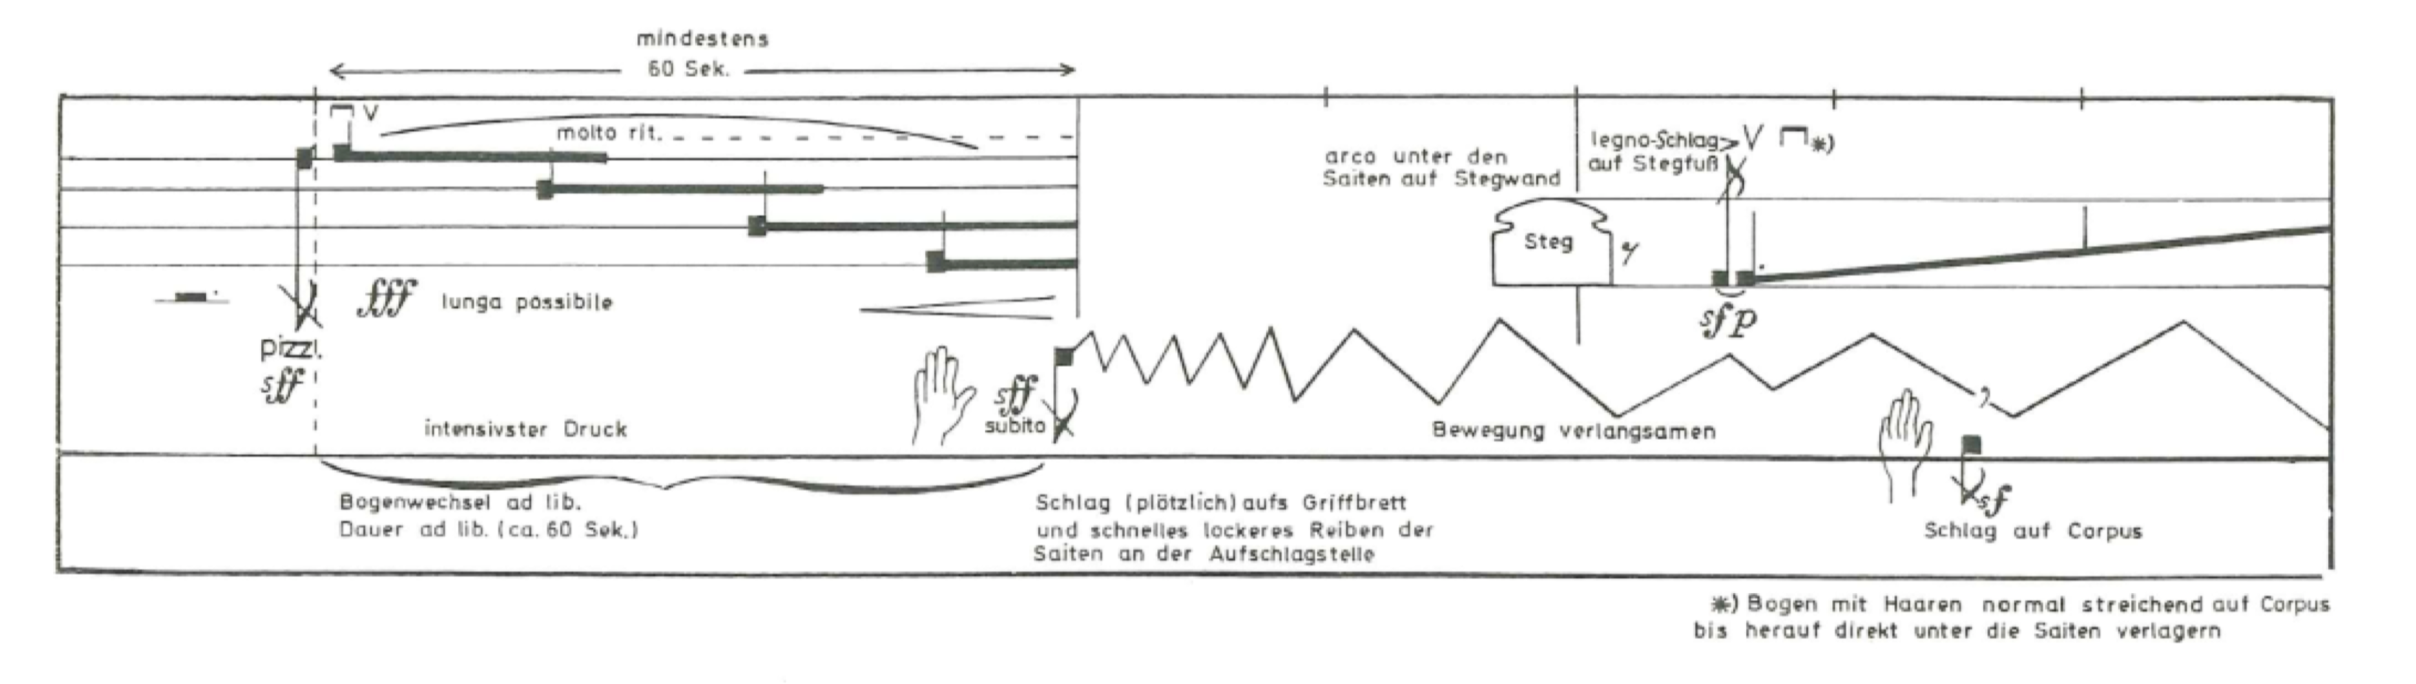
\includegraphics[width=1.\textwidth]{Lachenmann02.jpg}
\caption{particolare partitura \textit{Pression}}
\end{figure}

Penso che parta da questa base il lavoro sulla performance e da queste riflessioni si possano indicare tre punti principali del legame tra partitura e performance:

\begin{itemize}
\item{Lavoro tra performer e compositore. Ogni consiglio deve essere ben accetto e la possibilità di dialogo maggiore c'è nella stesura di una partitura chiara e vicina alle esigenze di uno strumentista. Più si matura e più si 
raggiunge una maggiore intelligibilità.}
\item{La presenza di gesti legati alla fisicità dello strumento e ad un legame tra movimento e simbologia.}
\item{Immaginare sia i gesti che l'andamento formale per evitare refusi e impossibilità fisiche performative.}
\end{itemize}

%************************************************

\section{Legame tra esecutore/performer 
e compositore}

\epigraph{Non si tratta di opprimere il pubblico con preoccupazioni cosmiche trascendenti. Che possano esservi chiavi profonde del pensiero e dell'azione in base alle quali leggere tutto lo spettacolo[...].
Tuttavia è necessario che queste chiavi esistano; e la cosa riguarda noi}{Antonin Artaud \\ Il teatro e il suo doppio}

Trovo affascinante il modo in cui i musicisti approcciano al loro strumento, ogni persona lo fa in modo differente e intimo. Studiando tecniche estese e subendo questa fascinazione, mi ritrovo continuamente a modificare la mia partitura e l'approccio con i musicisti che eseguono i miei pezzi diventa sempre complicato. Considero la stesura della partitura come un tramite per conoscersi ed interagire con chi la esegue. Ecco perché, mi capita spesso di rimettere mano ai miei spartiti per far sentire a proprio agio chi andrà a performare. Matteo Fracassi, studente del dipartimento di percussioni del Santa Cecilia, si è prestato a questo esperimento e ha deciso di intraprendere questo percorso conoscitivo addentrandosi nelle maglie della mia scrittura.

Il lavoro fatto su Sp.I.R.E. è stato leggermente diverso da quelli svolti in passato, perché essendo un nuovo strumento, ogni approccio non aveva riferimenti precedenti. Quindi si sono riscontrare delle difficoltà prima di tutto di scrittura: ogni gesto doveva essere rappresentato da un simbolo e soprattutto ogni timbro doveva legarsi ad una dinamica, una durata e ad un pitch (anche se non definito). Inoltre, avendo cinque molle e quattro placche non si può utilizzare una notazione standard, composta da uno spartito classico. Sicuramente, la notazione metronomica e l'utilizzo di accenti facilita la performance, così da dare risalto alle micro-forme interne e alla struttura del pezzo.

Un altro problema legato all'esecuzione è il contenuto timbrico e la dinamica dei gesti. Nell'approccio ad un nuovo strumento, non sempre le dinamiche hanno la stessa scala di valori tra chi le scrive e chi le legge, è opportuno infatti riportare degli esempi e se necessario suonarli noi stessi all'interprete. In alcuni casi è buono solfeggiare assieme delle parti. Ogni miglioramento richiesto dallo strumentista va valutato e prontamente segnato per poi riportarlo in partitura. Un apporto essenziale del percussionista è stato nella stesura della partitura base. Tutto si può migliorare e semplificare per facilitare l'esecuzione ed eliminare i refusi. L'interprete/performer si deve dedicare esclusivamente all'interpretazione del flusso formale. Inoltre, Il legame tra gesto e figura è strettamente correlato. Ogni gesto avrà bisogno di un riscontro sonoro adeguato per evitare che l'ammaliante timbrica di Sp.I.R.E. porti ad rapportarcisi in modo più improvvisativo che di studio. In pratica, ogni gesto rappresentato in partitura sarà la risultante sonora di un determinato timbro o di un determinato armonico.

Il performer deve possedere una capacità performativa estesa alla conformazione dello strumento,  deve avere la capacità di seguire una struttura compositiva salda e oltremodo precisa. Allo stesso modo, riuscire a districarsi nella lettura di una scrittura "quasi" libera. Per quasi, si intende, il saper unire tra loro i fraseggi che si incastrano, si restringono e si dilatano nel tempo (durata delle frasi) e nello spazio (estensione dello strumento) mantenendo un ictus costante che dia un'identità formale alla composizione.


% !TEX TS-program = pdflatex
% !TEX encoding = UTF-8 Unicode
% !TEX root = ../ArsClassica.tex

%************************************************
\chapter{La Composizione}
\label{chp:La Composizione}
%************************************************

Durante questi anni di accademia ho trasformato il mio rapporto con la composizione e il metodo di approccio agli strumenti e alle forme musicali. Dapprima ero in balia di un lungo
Il mio approccio alla composizione 
Come ogni mio attuale approccio a livello compositivo, ho cercato di creare una cellula di suoni disposti orizzontalmente, per poi lavorare sulla parte contrappuntistica. Dato che il nuovo strumento non ha pitch definiti è stato complicato lavorare su una cellula che al finire del suo svolgersi si potesse definire conclusa. Difatti ho cercato degli stratagemmi musicali, come gli accenti o la ricerca di determinati effetti timbrici (ad esempio attivazione di armoniche sugli estremi delle molle) che potessero diventare dei gesti musicali, sia a livello grafico che a livello d'ascolto. L'insieme di accento o di un numero determinato di gesti, vanno a formare le mie cellule ritmico-melodiche che interagiscono con la materia di cui è composta Sp.I.R.E. e quindi sempre in un rapporto 1:1 tra il ferro armonico delle placche e il metallo armoniche delle molle. Ogni cellula si sovrappone poi ad altre cellule simile in piccoli inserti contrappuntistici fatti di dilatazioni o restrizioni temporali del materiale sonoro. \\ 
Le cellule ritmiche sono formate da 7, 6, 5 e 11 eventi. La numerologia è legata al numero delle lettere che compongono nome e cognome dell'autore della poesia (7 = A-n-t-o-n-i-n, 6 = A-r-t-a-u-d), al numero delle sillabe del suddetto nome+cognome (5) e dal numero dei versi della poesia (11) sopra citata. \\
A livello compositivo compaiono delle cellule ritmiche che vanno a confluire in grossi nubi sonore. L'attinenza tra la scrittura e il gesto a volte è slegata, ma le piccole note e la tendenza ad una continuità ?notazionale? porta l?esecutore-performer a capire in quali punti vanno gestiti dei continuum. \\
Su ogni continuum vanno a frammentarsi altre cellule ritmiche. Ogni cellula si ripete, ma con piccole variazioni temporali, ogni gesto è riconosciuto sia nella semiografia che dal timbro percepito.
Sarà poi l?elettronica a legarsi agli accenti e agli incontri verticali delle varie cellule ritmico-melodiche. Si noterà poi, durante la performance, che alcune scelte gestuali presenti in partitura, sono connesse ad un movimento esclusivamente performativo: quasi teatrale.\\
Entrando nel merito della stesura compositiva, vado a sottolineare alcune peculiarità del movimento orizzontale e verticale delle voci. \\
Le varie parti di modulazione di frequenza e le interazioni ritmiche si incastrano seguendo un movimento verso le frequenze più alte. Se dall'inizio notiamo un'eccitazione delle sub-armoniche, qualità tipica della natura delle molle, in seguito si è spinti verso frequenze sempre più alte, cercando di andare di pari passo con una lettura temporale della poesia di Artaud: dalla vista dal basso verso l'alto degli astri (\textit{verres où cuisent les cerveaux / le ciel fourmillant d'impudeurs}) la notazione si erige, come grande rosone, verso armoniche generate sia dal materiale metallico composto dalle molle, sia da quello delle piastre. Si va ad indagare, quindi, \textit{nello} strumento (tramite una scrittura prettamente legata all'universo delle percussioni) sia textit{sullo} strumento (tramite l'utilizzo dell'elettronica). Tengo a sottolineare che l'amplificazione è colonna portante di tutto il brano, dato che tutte le elaborazioni e i contributi dell'elettronica sono diffusi esclusivamente tramite gli attuatori. L'amplificazione e qualunque elettronica a supporto della performance sono amplificate dai piezoelettrici e dai microfoni omnidirezionali. \\
Ogni contributo è un valore aggiunto a Sp.I.R.E. che si lascia 
\\
\\
La partitura ha come oggetto principale di scrittura, il processo con il quale sono stati ricercati i suoni: ogni gesto descritto graficamente, rappresenta il processo del timbro e della forma con la quale si vuole arrivare verso determinati frasi musicali, sia di natura percussiva che di natura timbrica.

\section{Materiali sonori}
\addcontentsline{toc}{section}{Materiali sonori}
Vitres de son è stata composta quindi su un sistema che si può definire sia \textbf{Acustico} che \textbf{elettronico}. \footnote{Acustica musicale e architettonica a cura di Sergio Cingolani, Renato Spagnolo UTET, 2004 Torino p. 3}

Tra i primi appunti ci furono molte stesure di una partitura che potesse legarsi: 
\begin{itemize}
\item{teatrale}
\item{tmondo sonoro}
\item{interazione}
\end{itemize}

Suoni di sfondo si adagiano su una superficie. Da lì diventano protagonisti, dal paesaggio sonoro, da un soundscape, fatto di piccoli grattati in \textbf{\textit{ppp}}, emergono forme che si incastrano con le figure ritmiche, ovvero le sillabe dei versi della poesia. Come se prendessero la forma di piccoli respiri, dati dalla lettura delle parole del poeta. Appare un \textit{dramma}, un enorme piaga che sottolinea Artaud in tutta la sua poetica giovanile e nei suoi lavori teatrali: non c'è più linguaggio parlato, divincolato dalla struttura principale di diffusione orale, ma solo suono. La musica, come la poesia, da suono di parole recitate, diventa figure ritimiche. \\
Nello stesso modo con il quale si applicano modifiche a livello di velocità di emissione delle sillabe durante una recitazione, così ho cercato di dar vita a delle variazioni nelle strutture ritmiche che si fondo con l'universo sonoro sottostante e vengono inghiottite dal soundscape. Ciò è reso possibile dalla natura del materiale: ogni passaggio delle dita o unghie sulle spire delle molle crea dei micro-glissati che formano maglie di suono che si fondono con le elaborazioni del live electronics. Ad un tratto appare, su frequenze gravi, una modulazione di frequenza. Questa FM, al suo interno ha dei piccoli movimenti spettrali, legati ad altrettanto piccole variazioni di parametri interni. Come affermava Xenakis:
\begin{quotation}
Una moltitudine di brevi \textit{glissandi} può dare l'impressione del continuo, come anche una moltitudine di \textit{pizzicati}\footnote{Iannis Xenakis, \textit{Universi del suono, Scritti e interventi 1955-1994} (a cura di Agostino Di Scipio), Ricordi S.r.l. e LIM Editrice S.r.l., 2003 \\}.
\end{quotation}




\section{Idea ritmico-melodica}
\addcontentsline{toc}{section}{Idea ritmico-melodica}

Affezionato alla poetica di Cage 
Le figure ritmiche servono a dare alla composizione un andamento strutturale. Ovvero, anche se molte figure non sono legate ad un preciso \textit{ictus}, servono comunque a creare degli incontri, ad esempio tra elettronica e parte strumentale o il movimento verticale di più voci. in \textit{Vitres de Son} in queste figure ritmiche sono nascoste le sillabazioni dei versi della poesia di Artaud, cercando di far intuire un andamento "vocale" delle parti. \\
Ho considerato utili tecniche di scrittura contemporanea legate al mondo degli idiofoni e all'universo dei cordofoni. \\
Per quanto riguarda la notazione, ho trovato, nel libro sulla semiografia contemporanea di Luigi Donora\footnote{Luigi Donora, \textit{Semiografia della nuova musica}, }, molte delucidazioni sulla creazione di figure ritmiche e simboli che potessero al meglio rappresentare il mio fine compositivo. Per fine compositivo intendo la possibilità di creare determinati timbri, riportando notazioni non canoniche ma che facessero capire la tipologia di gesto da utilizzare in un determinato frammento. Durante la stesura della partitura ha cambiato forma diverse volte. La prima partitura, infatti, era stata creata direttamente su una serie di pentagrammi, dove il si sopra al do centrale stava a simboleggiare il centro della molla e il movimento verso l'alto e verso il basso delle note rappresentava rispettivamente un movimento verso destra e verso sinistra (fig. ?)

%\begin{floatingfigure}{10cm}
%\mbox{\epsfig{file=fig_ritmica.jpg,width=9cm}}
%\small{\caption{\textit{particolare}}}
%\end{floatingfigure}

\begin{figure}[htbp]
\begin{center}
\includegraphics[]{../Graphics/fig_ritmica.jpg}
\caption{particolare}
\label{default}
\end{center}
\end{figure}

Le figure ritimiche servono a dare alla composizione un andamento strutturale. Ovvero, anche se molte figure non sono legate dad un ictus preciso, servono comunque a creare degli incontri, tra elettronica e parte strumentale o in alcuni punti nell?incontro verticale dipiù voci. All'interno di queste figure ritmiche sono nascoste le sillabazioni dei versi della poesia di Artau che prende
il nome del pezzo e rendono possibile una?vocalità? della composizione.

Ho considerato utili tecniche di scrittura contemporanea legate al mondo degli idiofoni e all'universo dei cordofoni. Per quanto riguarda il pentagramma, nella prima stesura era stato utilizzato per il movimento sulle corde, come in figura, si identifica il movimento da sinistra verso destra, con il movimento dal basso verso l'alto. In seguito, ogni movimento sul pentagramma, ogni forma che produceva un suono differente, si è trasformata in simbolo: ogni simbolo rappresenta quindi un gesto che si sviluppa in un determinato suono con un suo timbro specifico.
Saranno considerate utili tecniche di scrittura contemporanea, legata al mondo delle percussioni per lo strumento di nuova creazione. Il pentagramma diventa la base di un movimento sull'asse orizzontale dello strumento. Il pentagramma con centro sul Si sopra al Do centrale, nella prima stesura, ed un uno rigo unico con centro nel rigo stesso nella seconda, rappresentano graficamente una determinata molla che sarà nominata in legenda con la lettera M. Per rendere più semplice ogni movimento e ogni incastro ritmico, ho redatto degli esempi che vengono esplicati in legenda tramite una didascalia, così da migliorare l'approccio con la partitura e di conseguenza con l'iper-strumento.

\section{Gestualità}
\addcontentsline{toc}{section}{Gestualità}

Sarà quindi il gesto ad essere la base della prosodia interna, ogni legame con il gesto successivo sarà studiato per dare un movimento sia alle voci, che possono essere fino a 3 simultanee, come si nota nell'ultima pagina della partitura, dove la punta dell'arco si muove su una placca (P2), il centro dell'arco si muove su M5 e la base dell'archetto percuote M4 chiudendo in un crescendo dinamico.
L'utilizzo di simboli vicini al mondo della musica classica mi ha aiutato ad adeguare uno strumento del quale non abbiamo letteratura, verso una nuova scrittura, tutto ciò è la base poi della musica contemporanea, ovvero, ogni nuovo gesto è l'evoluzione di un gesto appartenente a musica più antica. Alcuni movimento dell'archetto infatti stanno a simboleggiare i gesti della mano o dell'archetto, come avveniva in passato per la musica gregoriana, con i melisimi legati al movimento delle mani dei direttori di coro della tradizione.

\section{Macro-forma}
\addcontentsline{toc}{section}{Macro-forma}

Il lavoro è svolto sulla poesia di Artaud. Come se ogni gesto si collegasse ad una parafrasi immaginifica e musicale della poesia del drammaturgo francese. \\

\begin{quotation}
\textit{Vitres de son où virent les astres \\
verres où cuisent les cerveaux \\
le ciel fourmillant d'impudeurs \\
dévore la nudité des astres. \\ \\ \\}
\end{quotation}





\section{La legenda}
\addcontentsline{toc}{section}{La legenda}
La partitura si apre con il progetto di Sp.I.R.E., per poterlo riprodurre ed utilizzare materiali affini.\\
Per facilitare la lettura della partitura elettroacustica, ho preferito dividere la legenda in quattro blocchi fondamentali:
\begin{itemize}
\item{Il primo blocco comprende la tipologia di battenti, utilizzati anche nella musica classica, ma \textit{numerati}, per facilitare i cambi in partitura, dato che per ogni battente abbiamo un'eccitazione diversa delle molle e un timbro differente.}
\item{Il secondo blocco delinea la notazione e la simbologia presente in partitura}
\item{Il terzo blocco ha al suo interno degli esempi che facilitano lo studio degli incastri ritmici}
\item{L'ultimo blocco comprende tutti i simboli e i gesti legati all'elettronica (pedali, variazioni di parametri, elaborazioni)}
\end{itemize}


\begin{center}
\begin{minipage}[c]{1.\textwidth}
\includegraphics[width=0.4\textwidth]{legenda1.jpg}
\end{minipage}
\end{center}


\begin{center}
\begin{minipage}[c]{1.\textwidth}
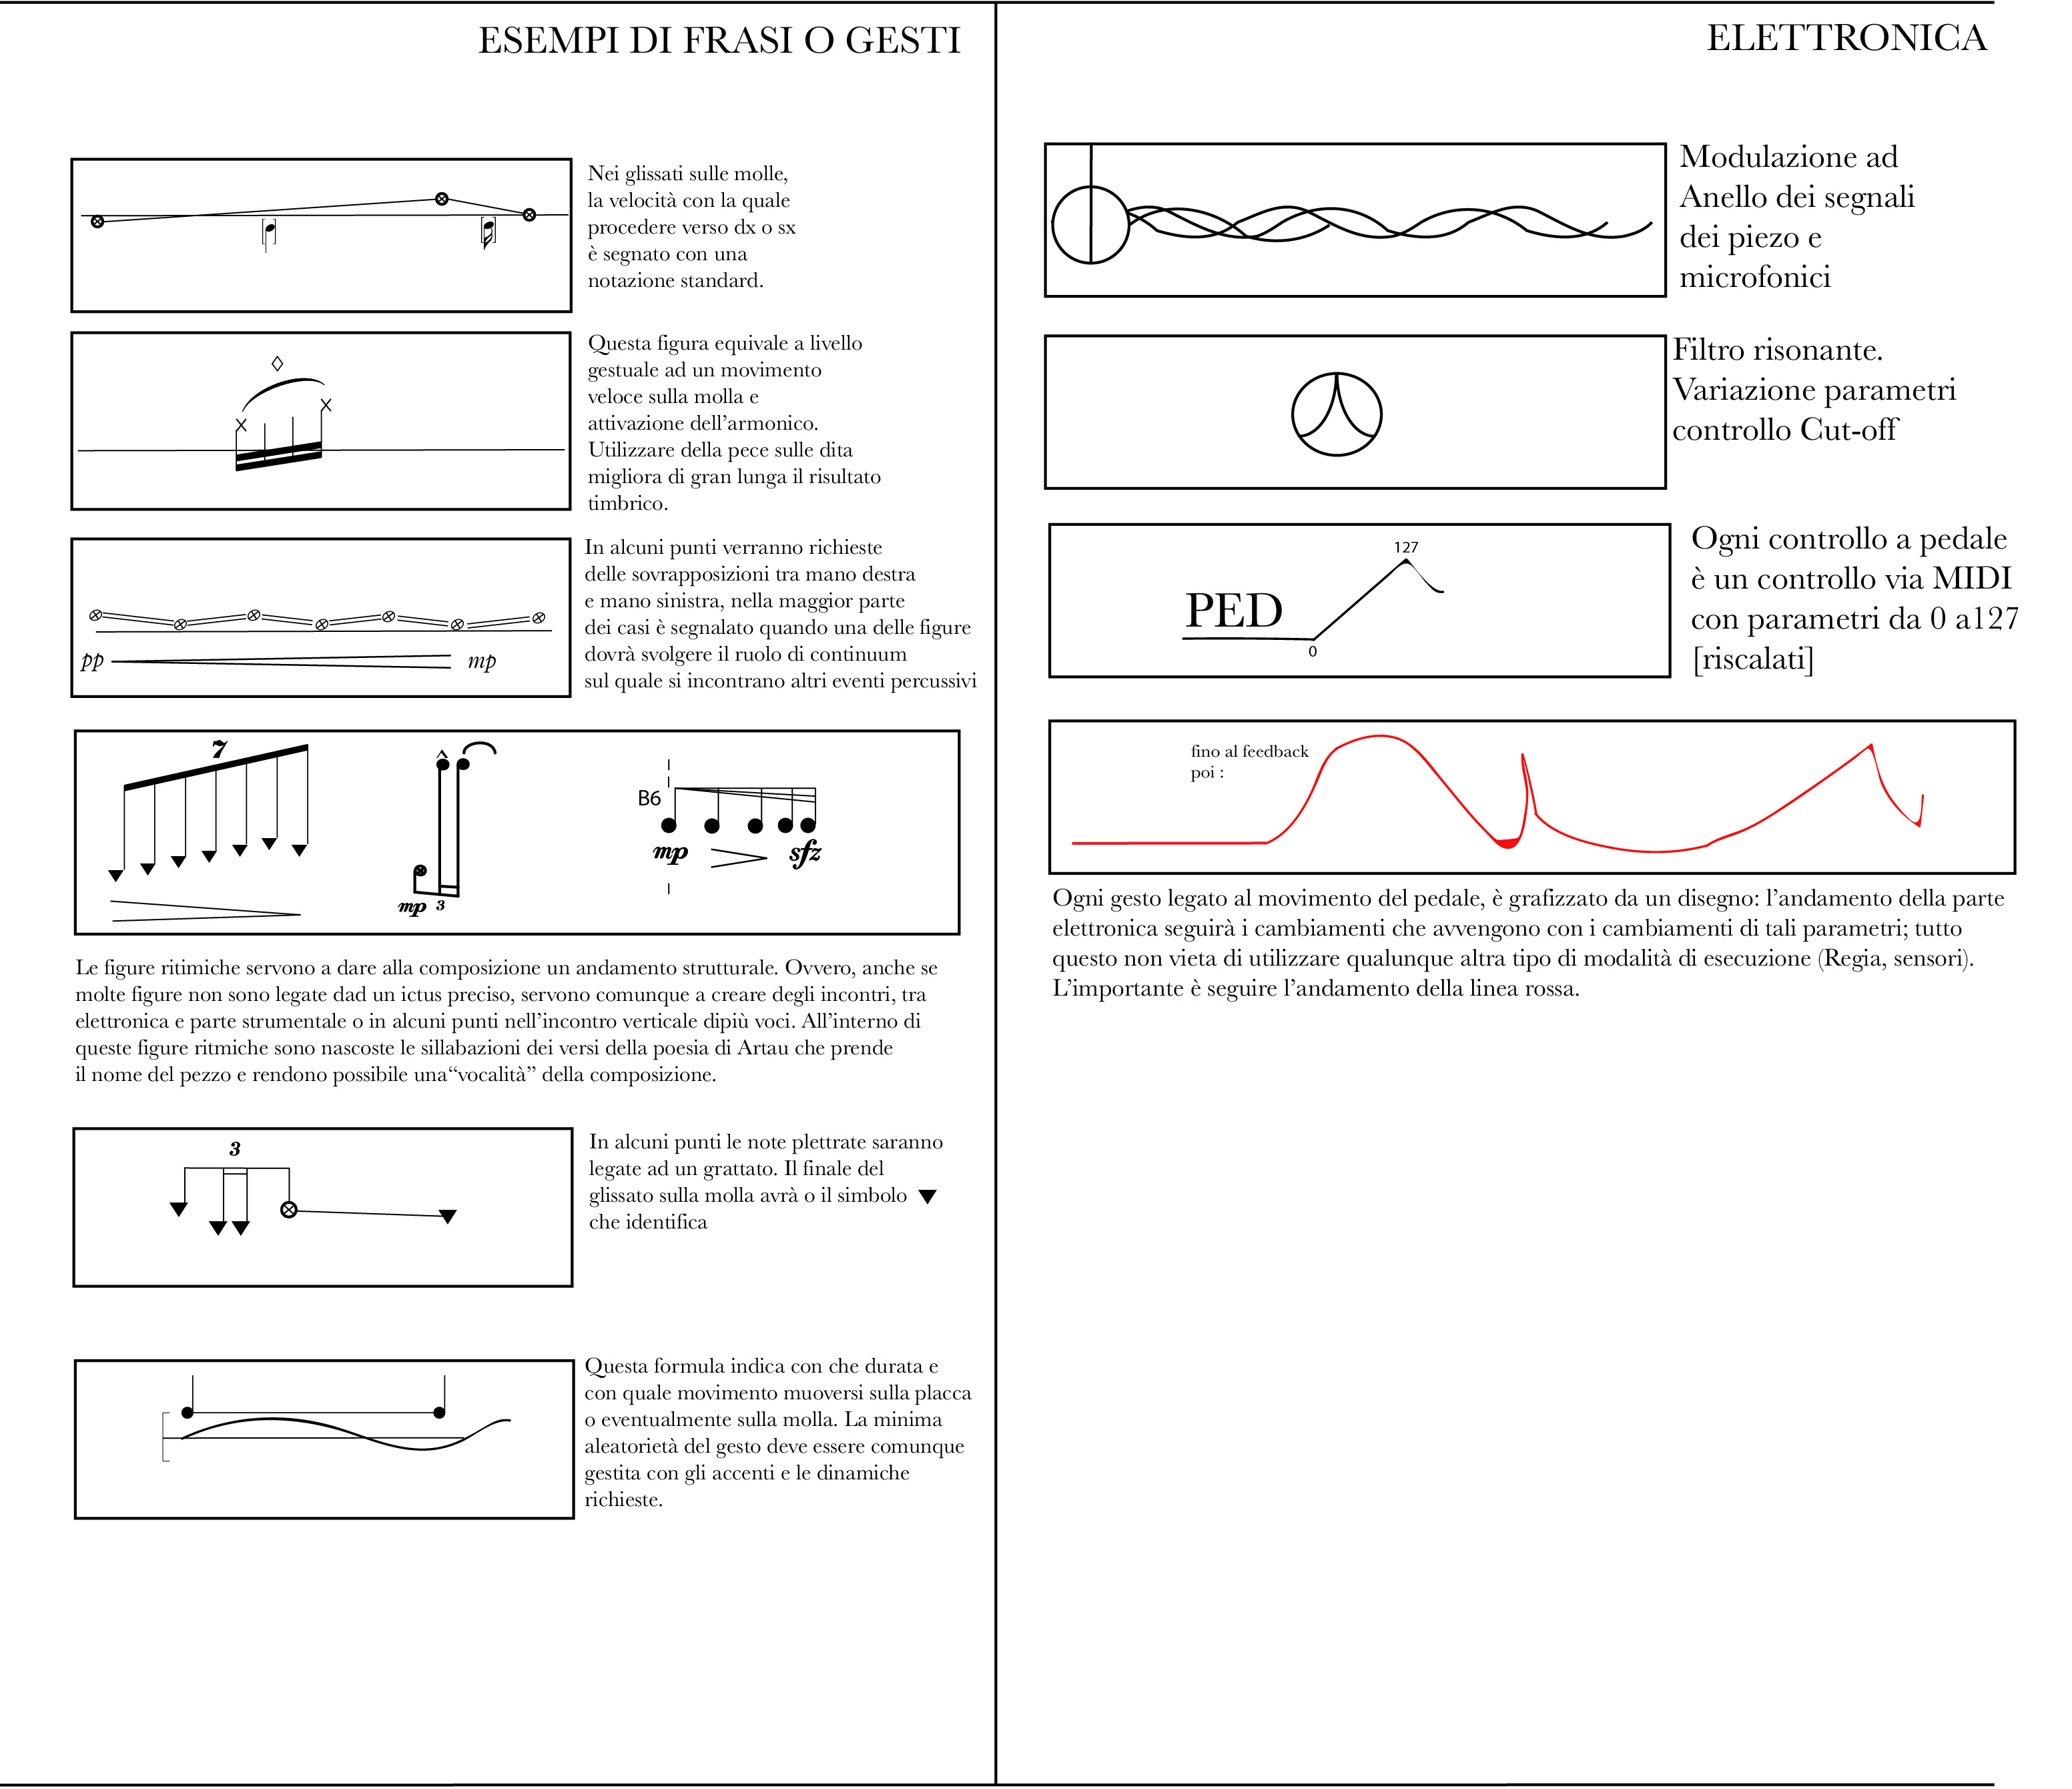
\includegraphics[width=0.6\textwidth]{legenda2.jpg}
\end{minipage}
\end{center}


\section{Algoritmi}
\addcontentsline{toc}{section}{Algoritmi}
\begin{center}
\begin{minipage}[c]{1.\textwidth}
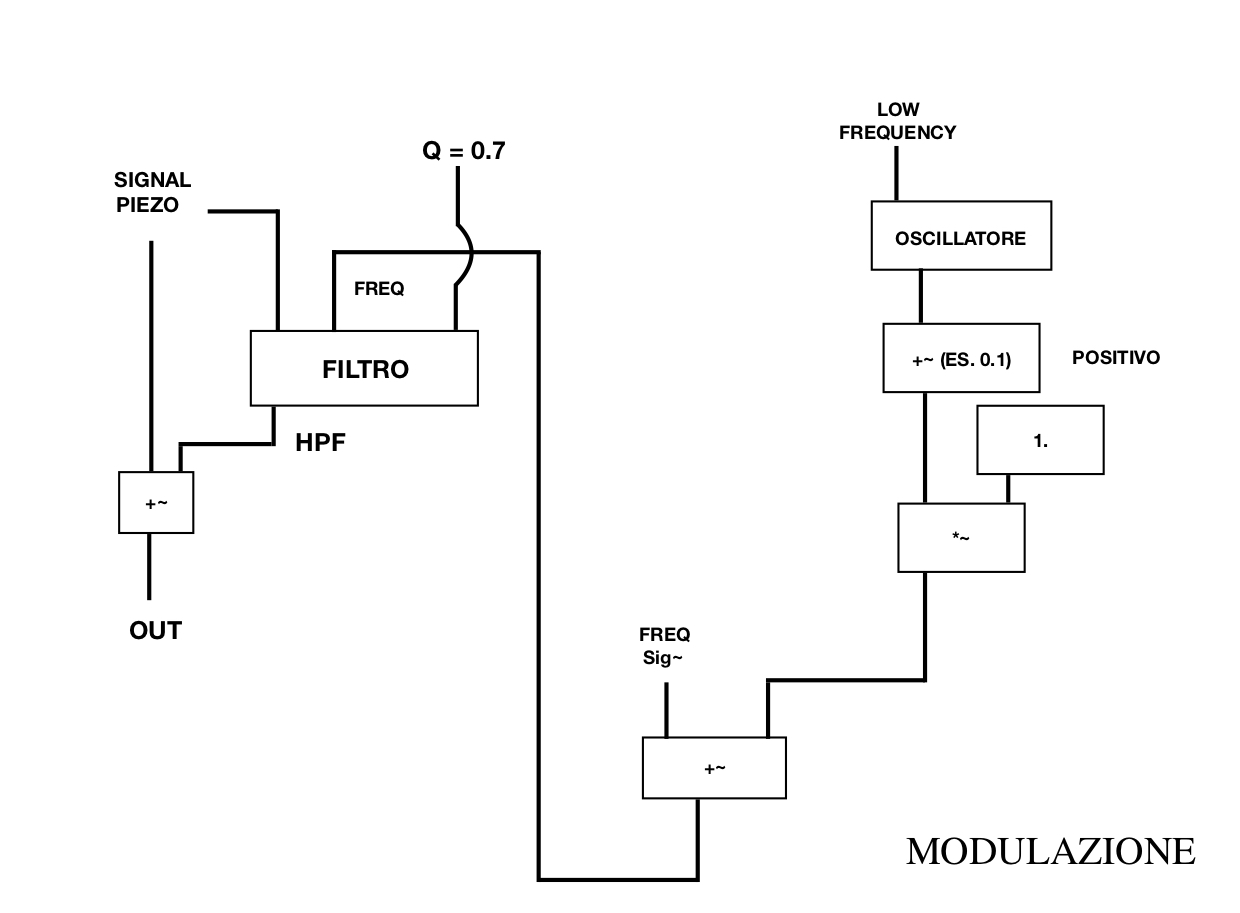
\includegraphics[width=1.\textwidth]{algo_1.jpg}
\end{minipage}
\end{center}
\begin{center}
\begin{minipage}[c]{1.\textwidth}
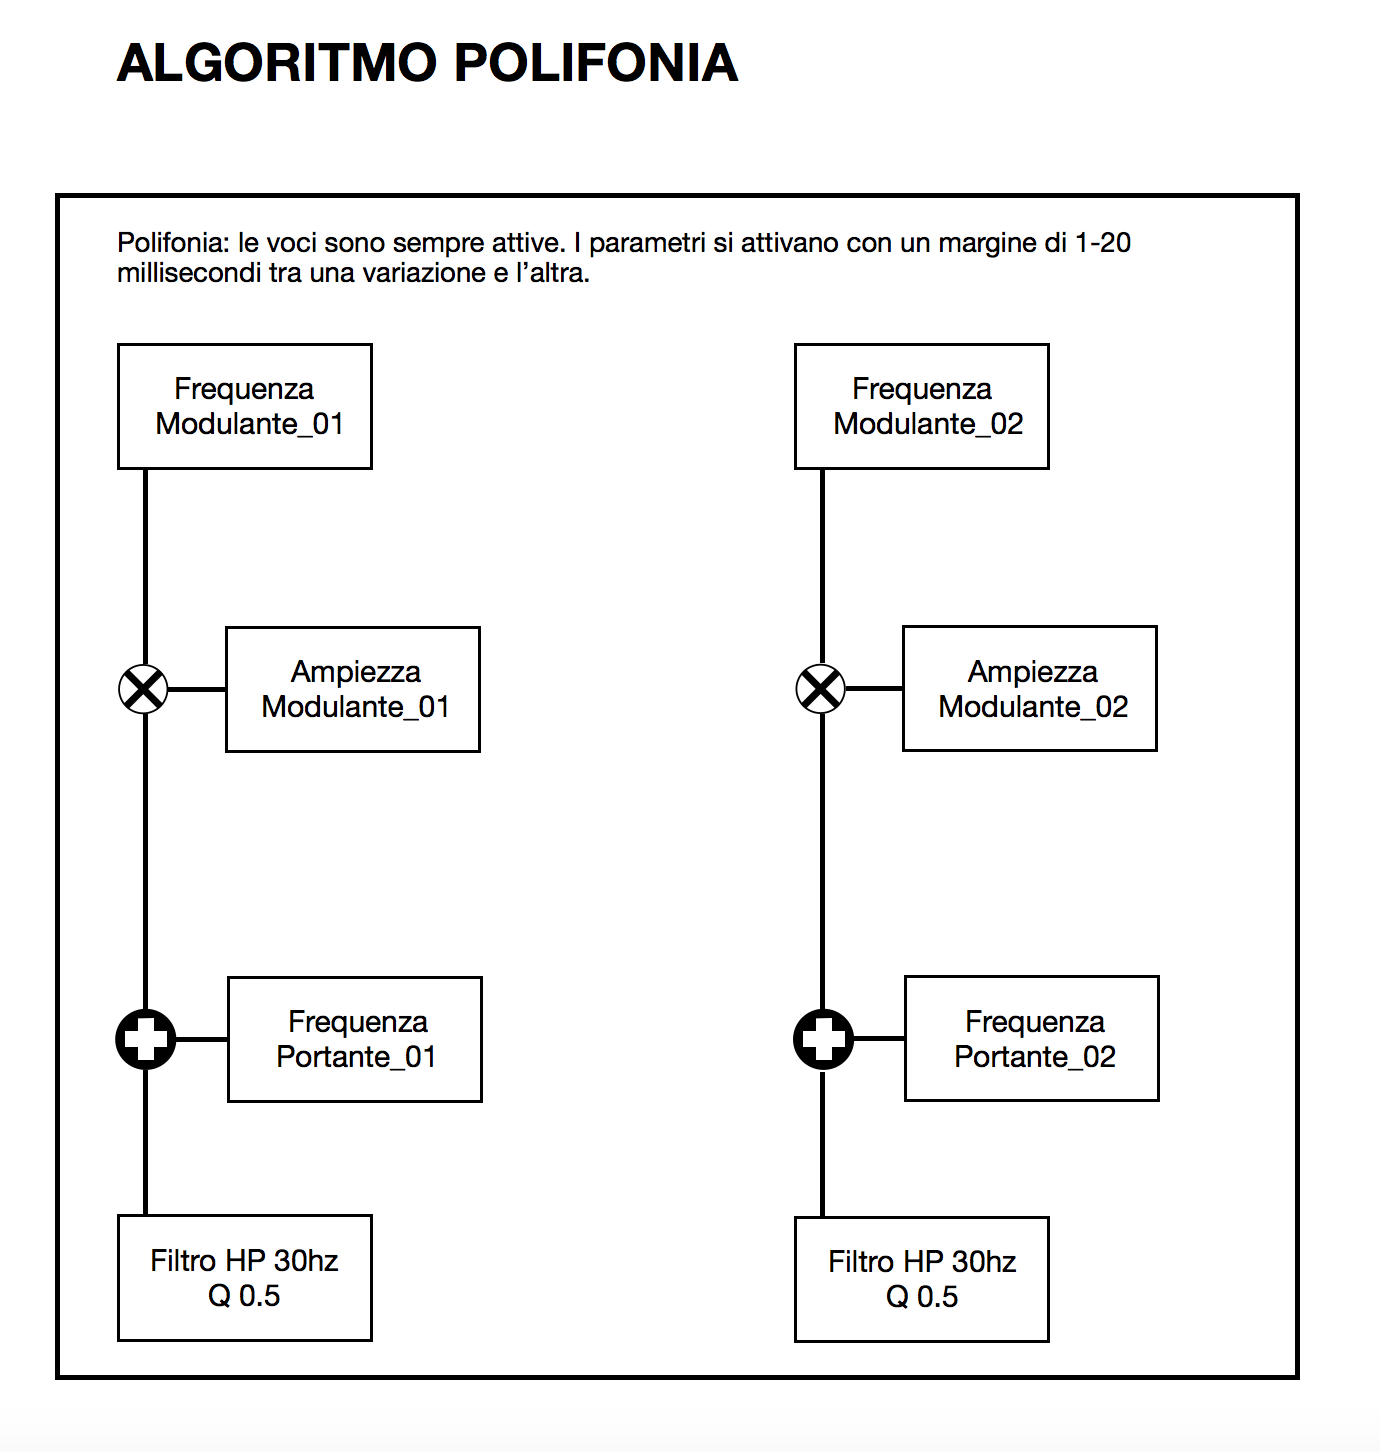
\includegraphics[width=1.\textwidth]{algo_2.jpg}
\end{minipage}
\end{center}


\section{Pedaliera}
\addcontentsline{toc}{section}{Pedaliera}

Pedaliera. Dopo aver studiato il funzionamento ho notato che ogni pulsante numerato era assegnato ad un NOTE on, come una normalissima pedaliera midi per organo. La fortuna è che ogni pulsante equivale a note inerenti al numero presente sulla pedaliera (es. note-on 1 = tasto 1 pedaliera). Quindi essendo identiche, ho solo dovuto trasformare ogni note-on in un ?lancio-scena? sul mio software di utilizzo (max-msp). Questo mi ha facilitato lo studio con il performer che può riprovare ogni scena senza dover ripetere temporalmente la sequenza in partitura, ovvero può passare ad esempio dalla scena 1 alla scena 6 senza dover ripercorrere tutte le scene presenti tra quelle menzionate. Questo facilita la prova per ogni singolo rigo.


% !TEX TS-program = pdflatex
% !TEX encoding = UTF-8 Unicode

%************************************************
\chapter{La ricerca dei materiali (elettromeccanici)}
\label{chp:La ricerca dei materiali (elettromeccanici)}
%************************************************

Le molle prese in esame sono state a (trazione) e a (compressione).
Dopo varie ricerche fatte anche su materiali presenti al CRM, la soluzione per l'esecuzione del pezzo è la seguente:

\begin{itemize}
\item{L'acciaio armonico è risultato il materiale migliore per il mio utilizzo perché a diametri bassi di filatura si possono avere grandi o piccoli diametri per le spire e il risultato non cambia.}
\item{Ogni molla, se ha un diametro compreso tra 0.1 e 0.2 cm, si ottiene una grande manovrabilità a livello di flessione e tensione. Da sottolineare che vanno utilizzate solo ed esclusivamente le \underline {Molle a Trazione}; perché in estensione hanno rigidità minime anche per lunghezze pari al doppio della loro lunghezza a riposo.}
\end{itemize}

\begin{table}[htp]
\caption{Tipologia di molle utilizzate:}
\begin{center}

\begin{tabular}{cp{2cm}p{2cm}p{.2cm}p{2cm}} \textbf{MOLLA}&\textbf{DIAM.}&\textbf{LUNGH.}\\
\hline \textit{in centimetri} \\
\hline 5&2&20\\
\hline 4&1.2&20\\
\hline 3&1.5&20\\
\hline 2&0.8&8\\
\hline 1&0.6&8\\
\end{tabular}

\end{center}
\label{default}
\end{table}%



\begin{table}[htp]
\caption{Perimetro delle lastre:}
\begin{center}

\begin{tabular}{cp{2cm}p{2cm}p{.2cm}p{2cm}} \textbf{PIASTRA}&\textbf{LARGH.}&\textbf{LUNGH.}\\
\hline \textit{in centimetri} \\
\hline 1&20&20\\
\hline 2&15&20\\
\hline 3&15&20\\
\hline 4&20&20\\
\end{tabular}

\end{center}
\label{default}
\end{table}%

%************************************************

\section{Progettazione e supporto di tiraggio}

% \begin{figure}[htbp]
%        \centering
%        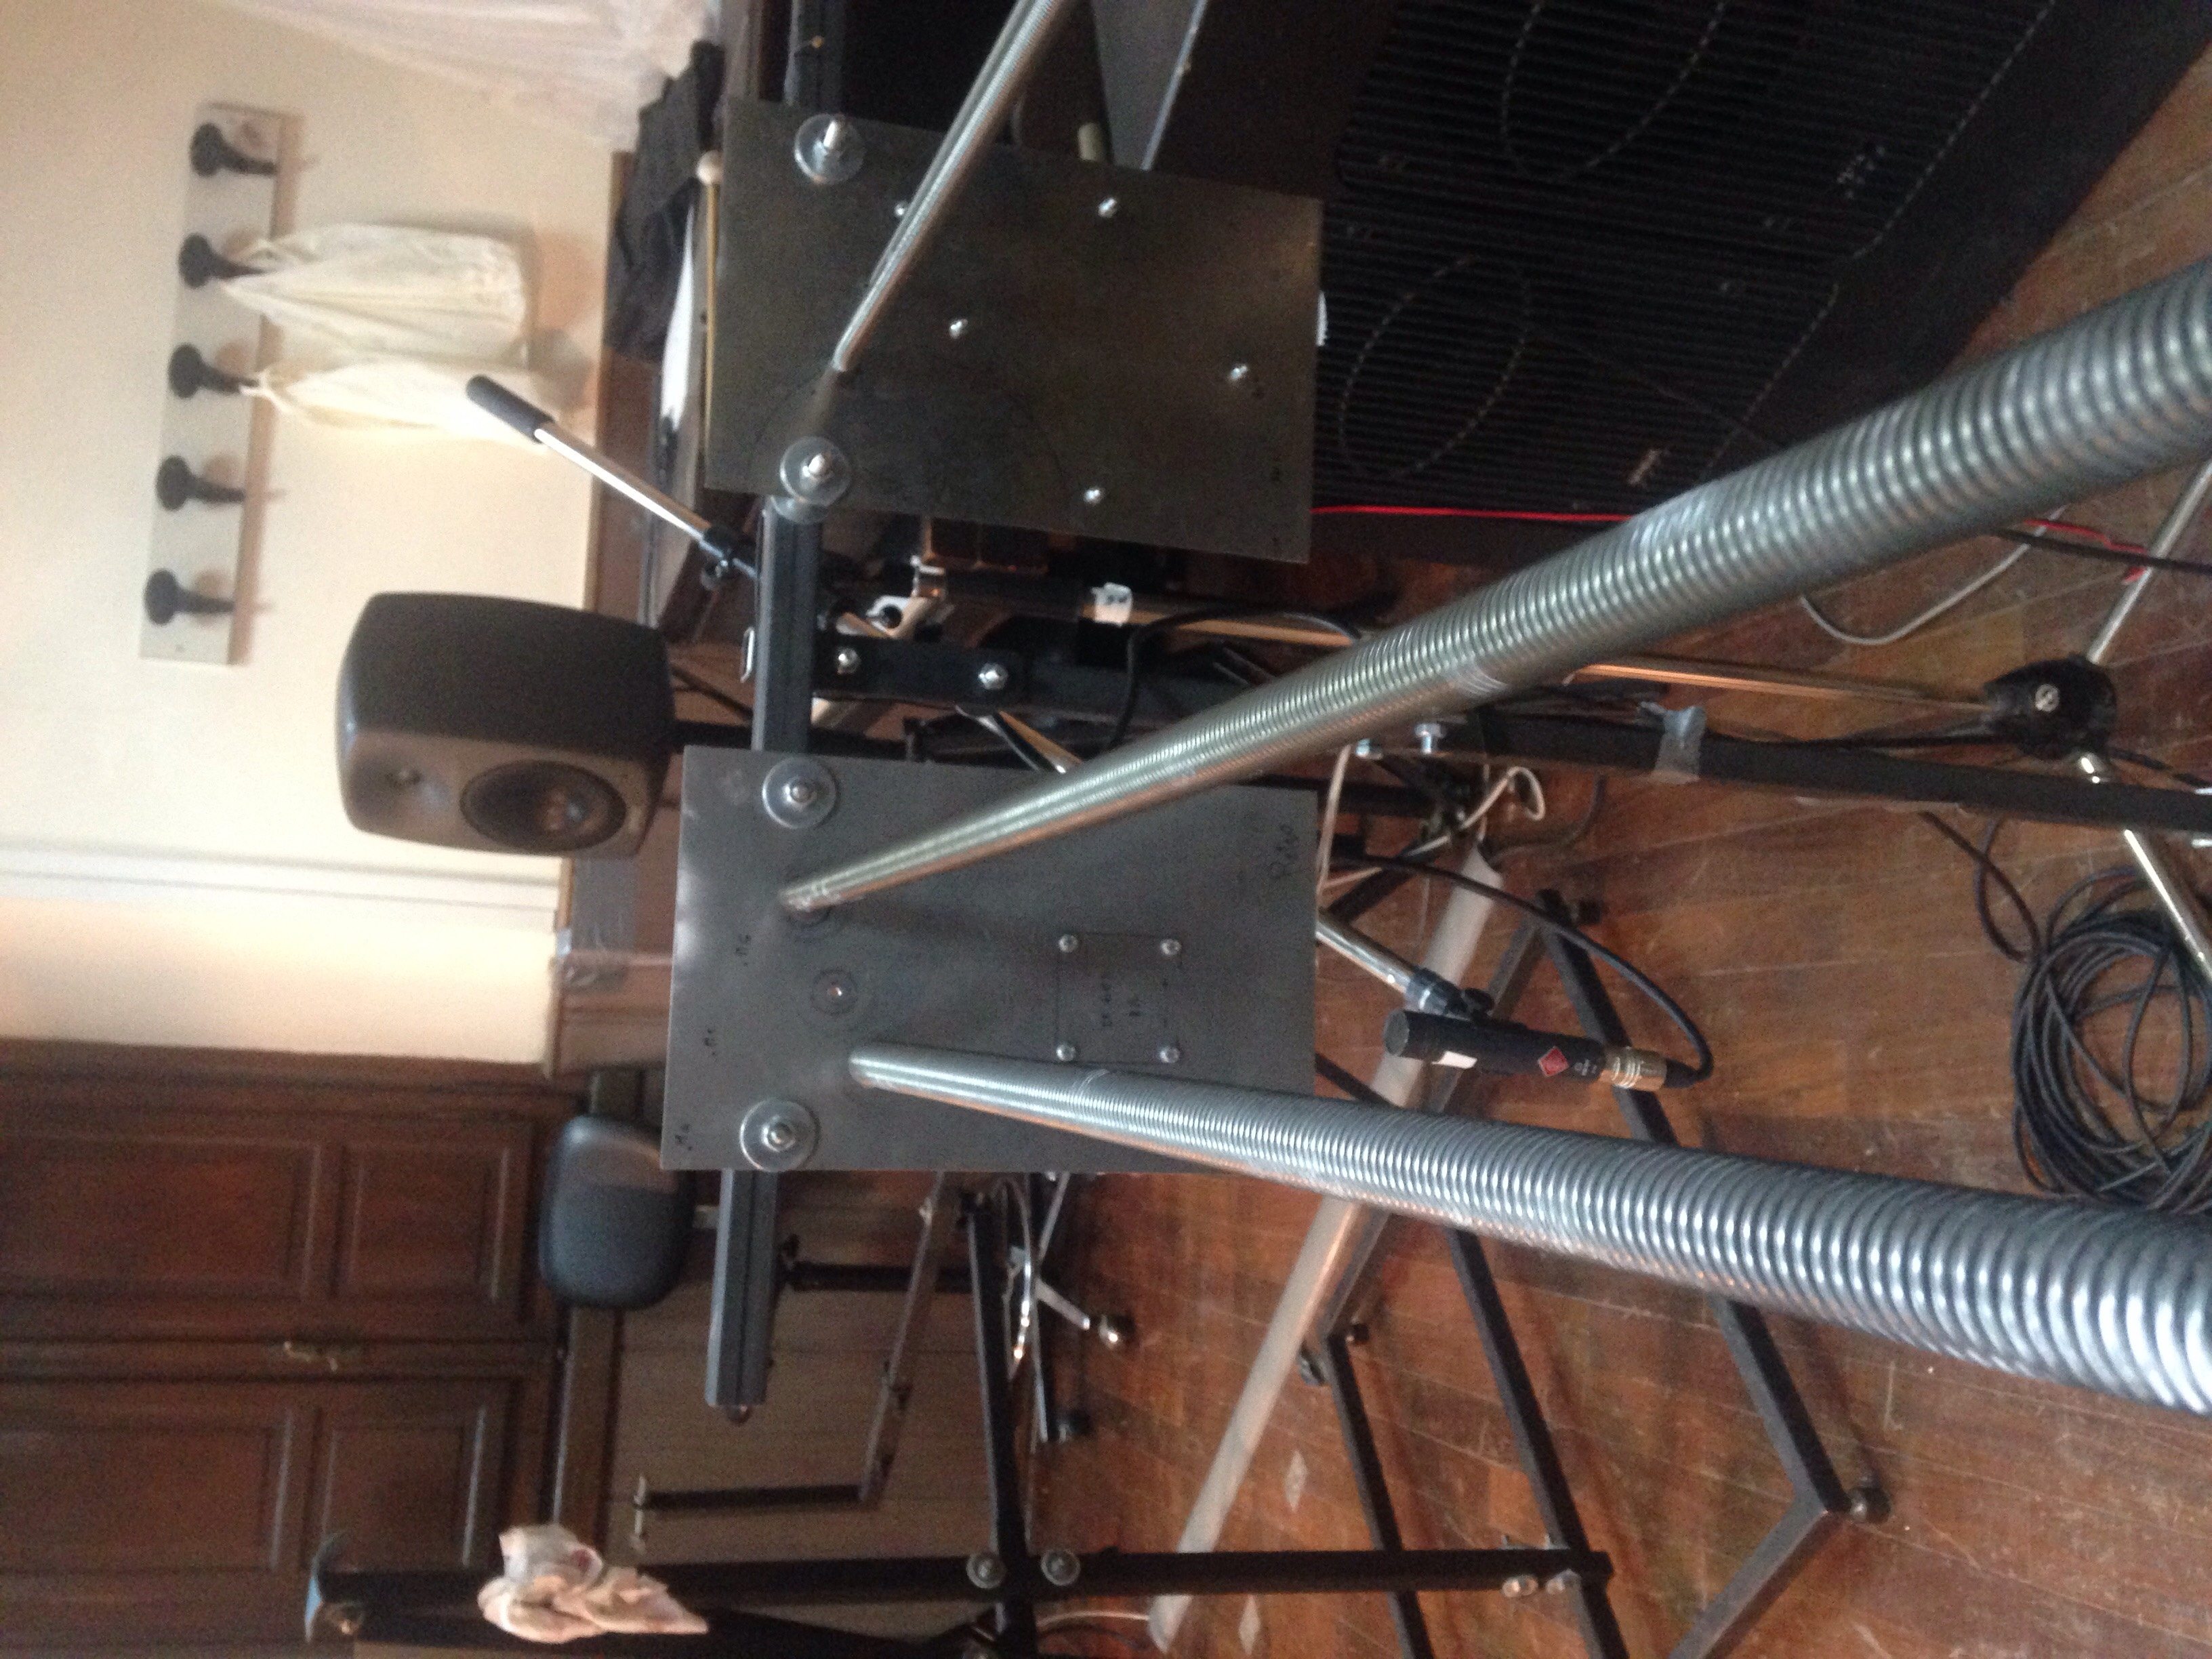
\includegraphics[height=6cm, width=5cm, angle=0,
%          keepaspectratio]{Spire2.jpg}
%\end{figure}

\begin{figure}[htbp]
\begin{center}
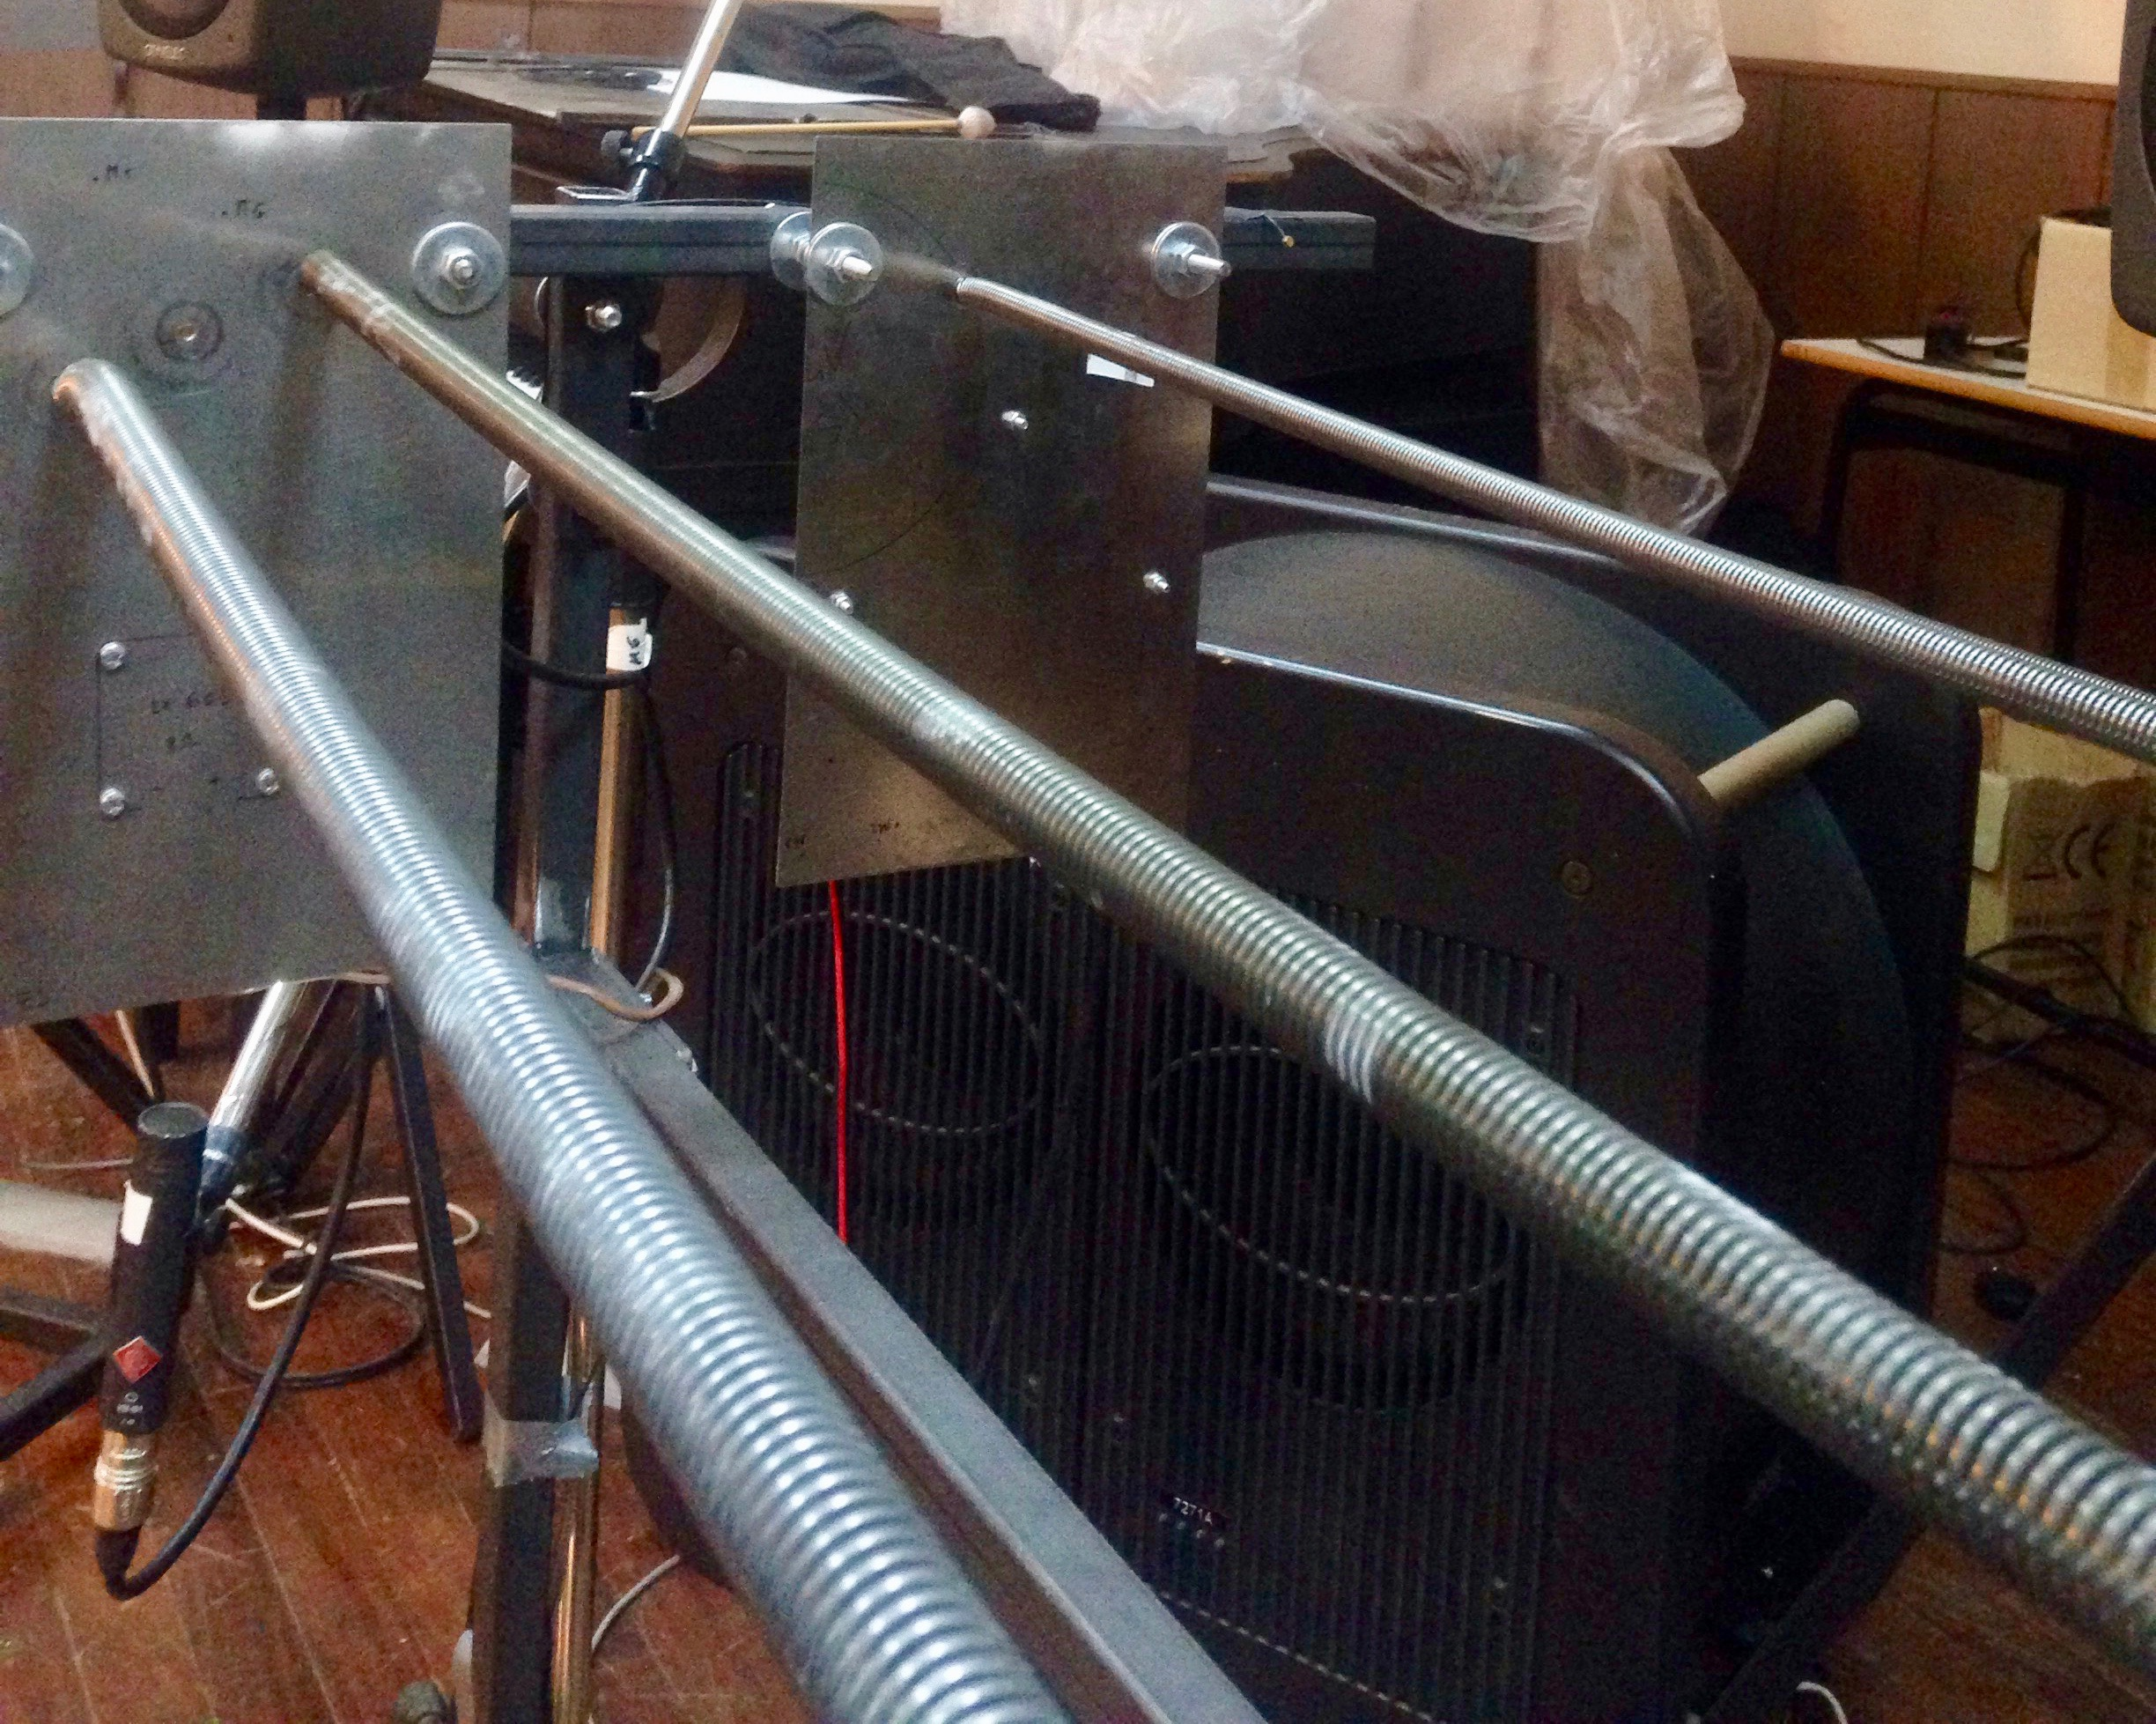
\includegraphics[width=.99\textwidth]{Spire3cc.jpg}
\caption{Particolare delle molle più esterne, quelle più gravi (Molla 4 e 5)}
\label{default}
\end{center}
\end{figure}

Le molle a trazione possono arrivare ad una forza di tiraggio pari anche a 100 chili. Per questo l'utilizzo di un basamento adeguato, creato su misura da un fabbro, è la soluzione a qualunque problema relativo al paragrafo successivo: il fissaggio di attuatori e molle.
Il basamento è stato creato, come scritto in precedenza, grazie all'aiuto di un assistente del Centro di Ricerche Musicali, Leonardo Mammozzetti, che ha visionato e modificato il progetto. Il supporto è in ferro e come in figura \label{fig:basamento} notiamo i punti di saldatura, segnati in verde. In basso a destra il nome degli attuatori utilizzati, la marca è \emph{Visaton}.

\begin{figure}[htbp]
\begin{center}
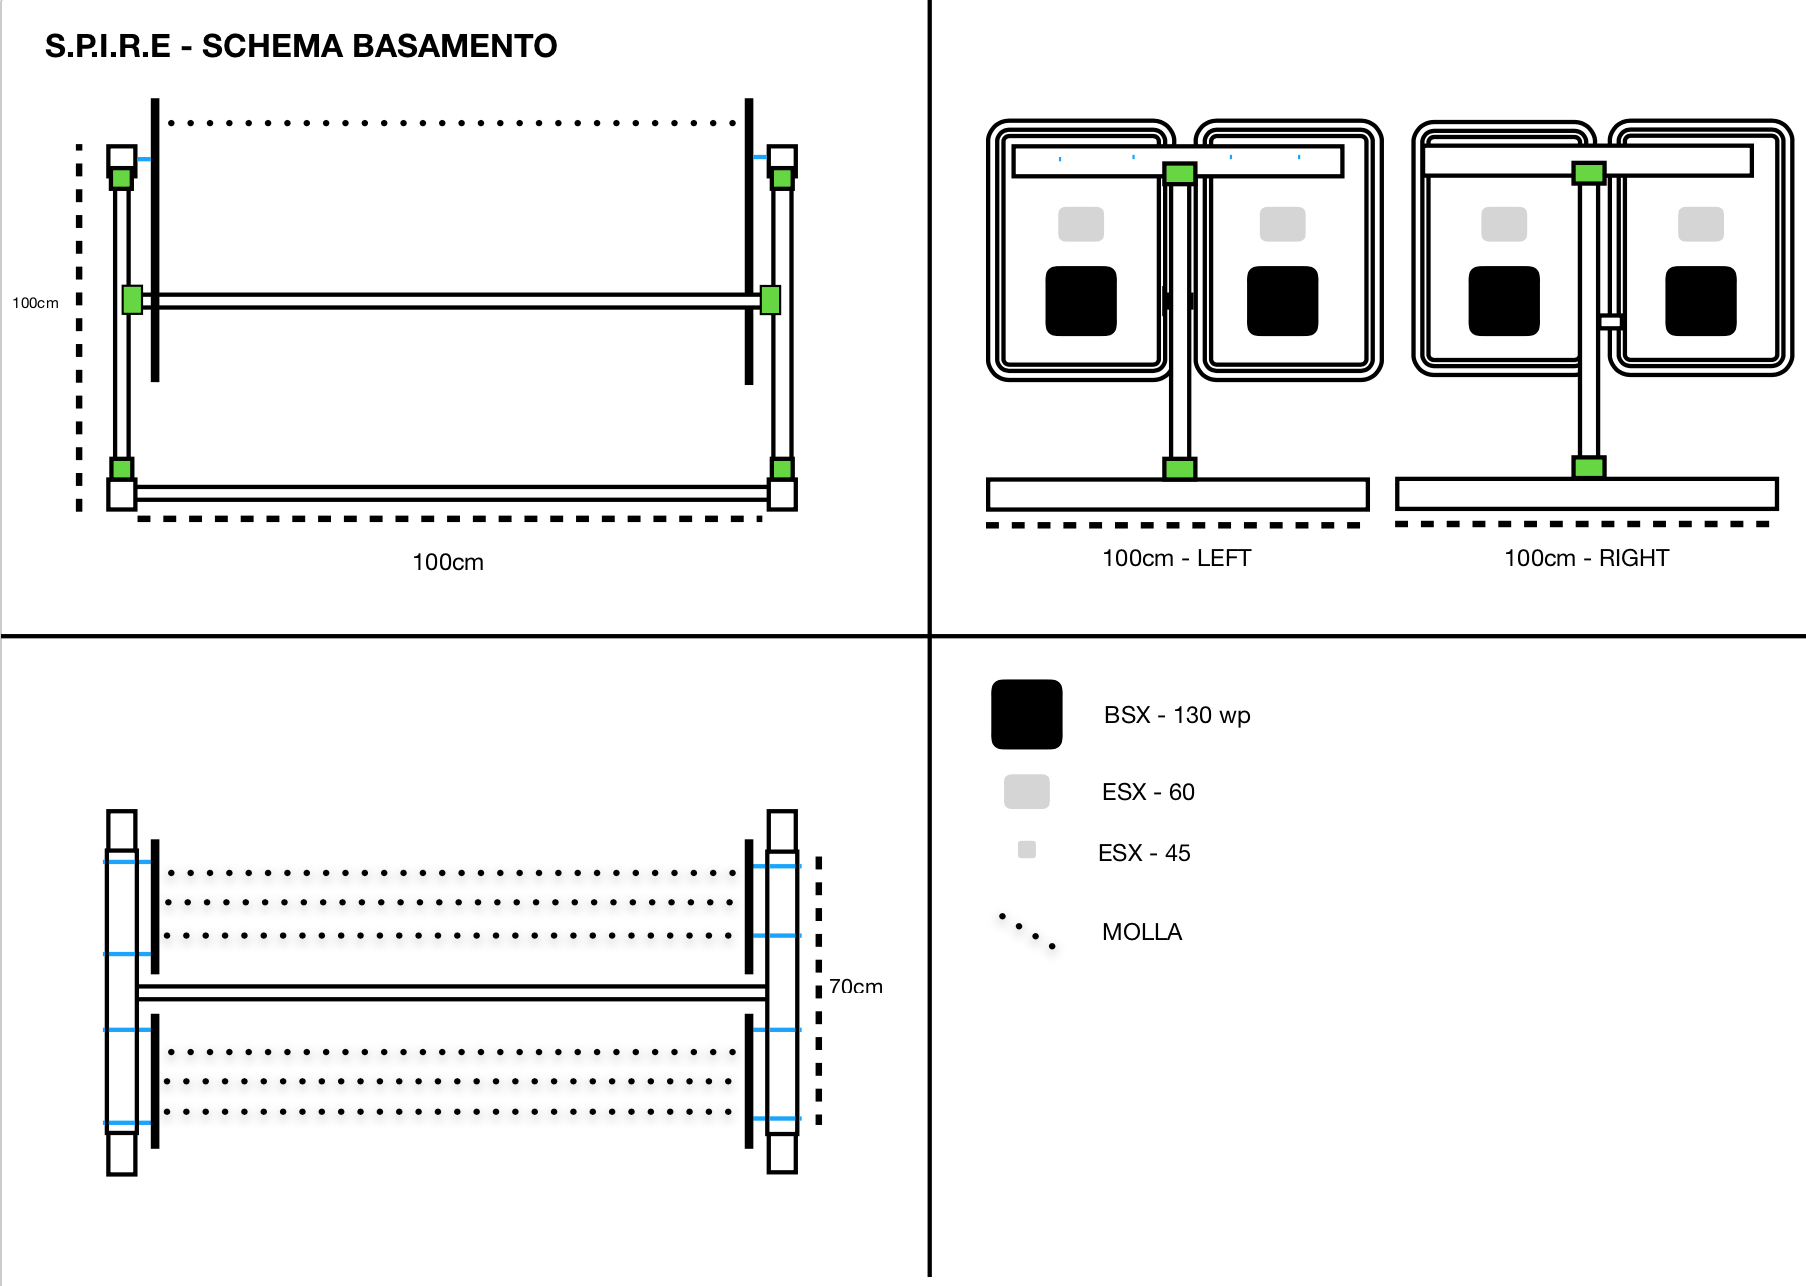
\includegraphics[width=.99\textwidth]{Basamento.jpg}
\caption{Basamento dello strumento}
\label{basamento}
\end{center}
\end{figure}

%\begin{figure}[htbp]
%        \centering
%        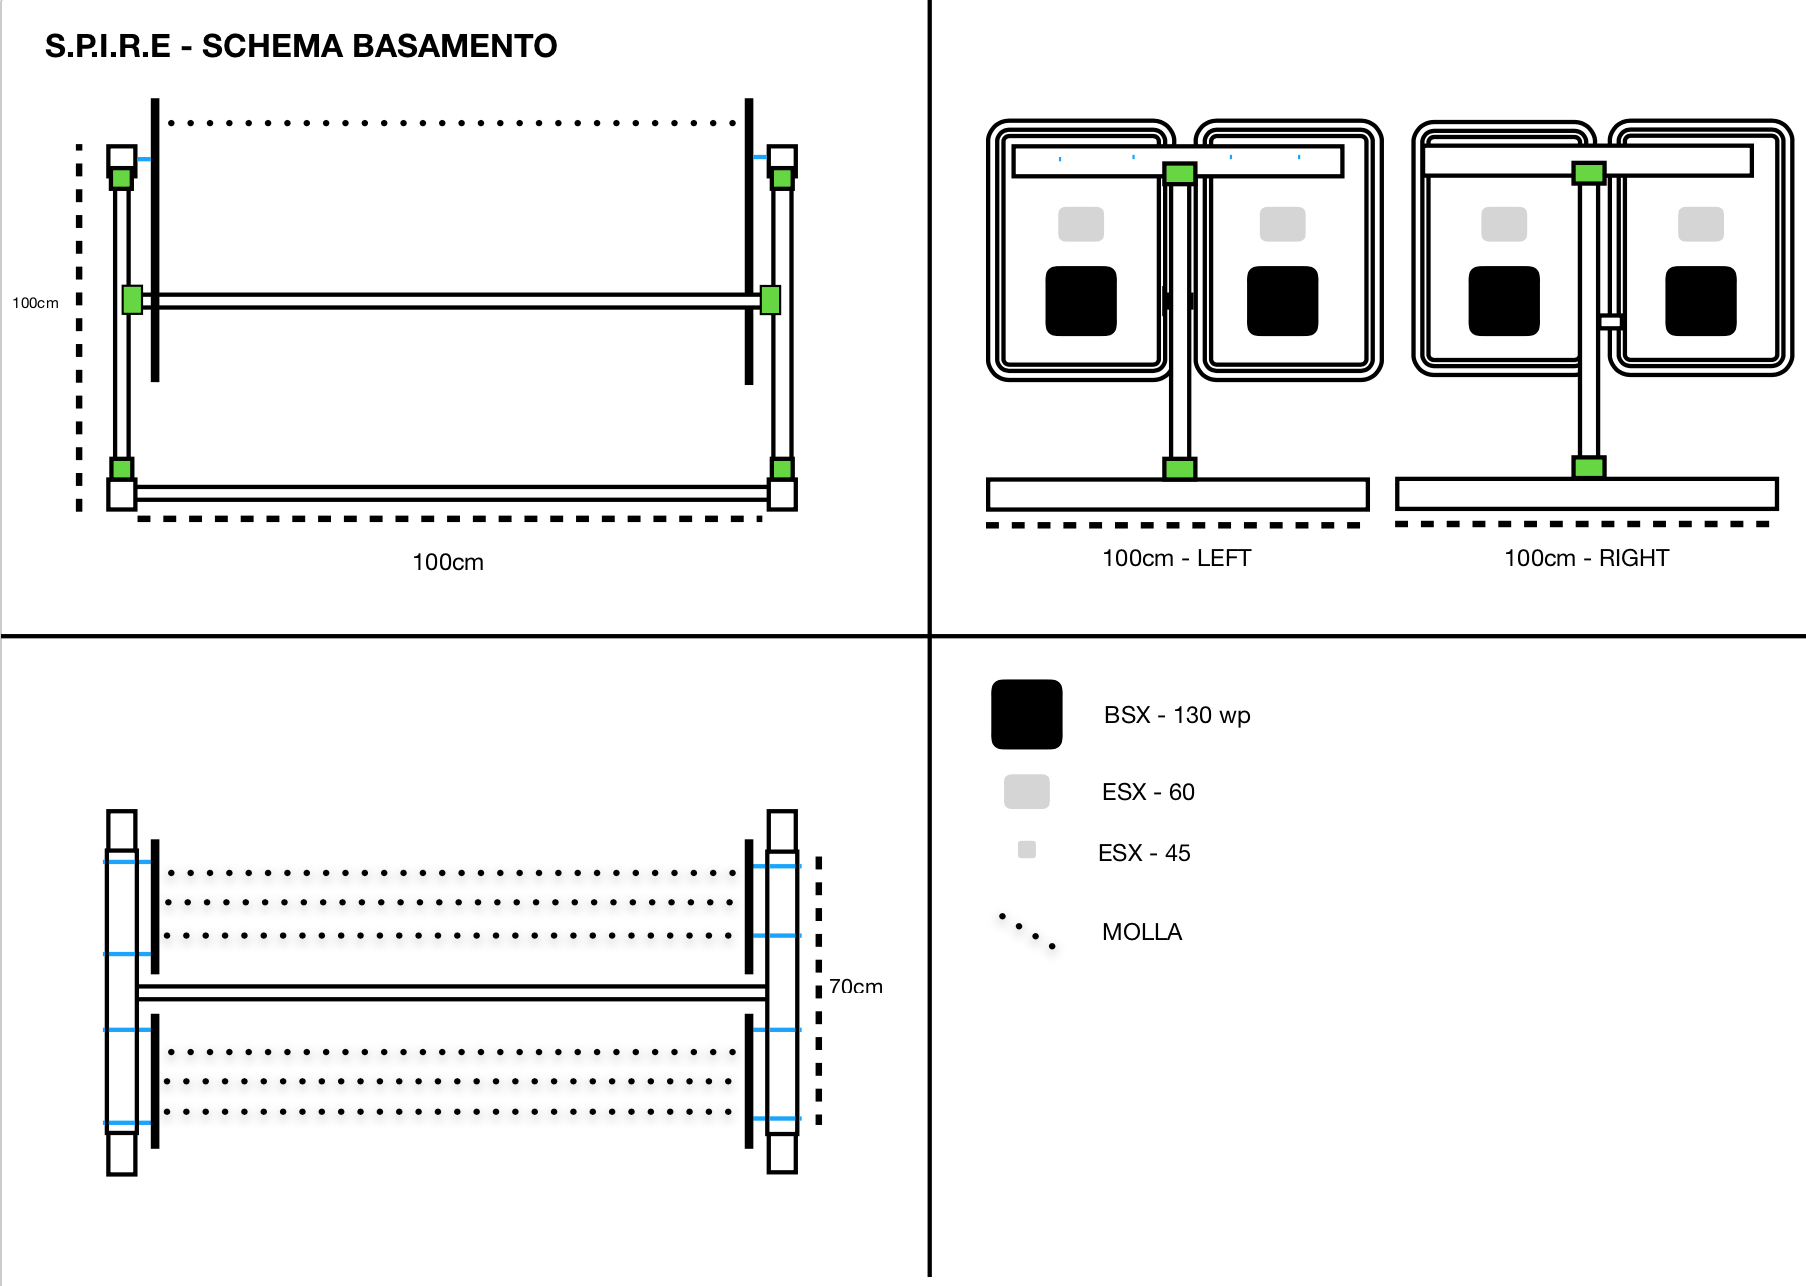
\includegraphics[height=15cm, width=15cm,
%          keepaspectratio]{Basamento.jpg}
%\end{figure}

Le molle a trazione sono state fissate come in figura, facendo dei buchi sulla lamiera e tese, tutto nella stessa lunghezza, per rendere possibile uno studio omogeneo su materiali diversi che rispondono diversamente al tocco e all'eccitazione mediante attuatori.\\
Si è notato che ogni molla si comporta differentemente a seconda del diametro delle spire, della robustezza del materiale e, ovviamente, del diametro del cavo in acciaio armonico.

%
%\begin{figure}[htbp]
%        \centering
%        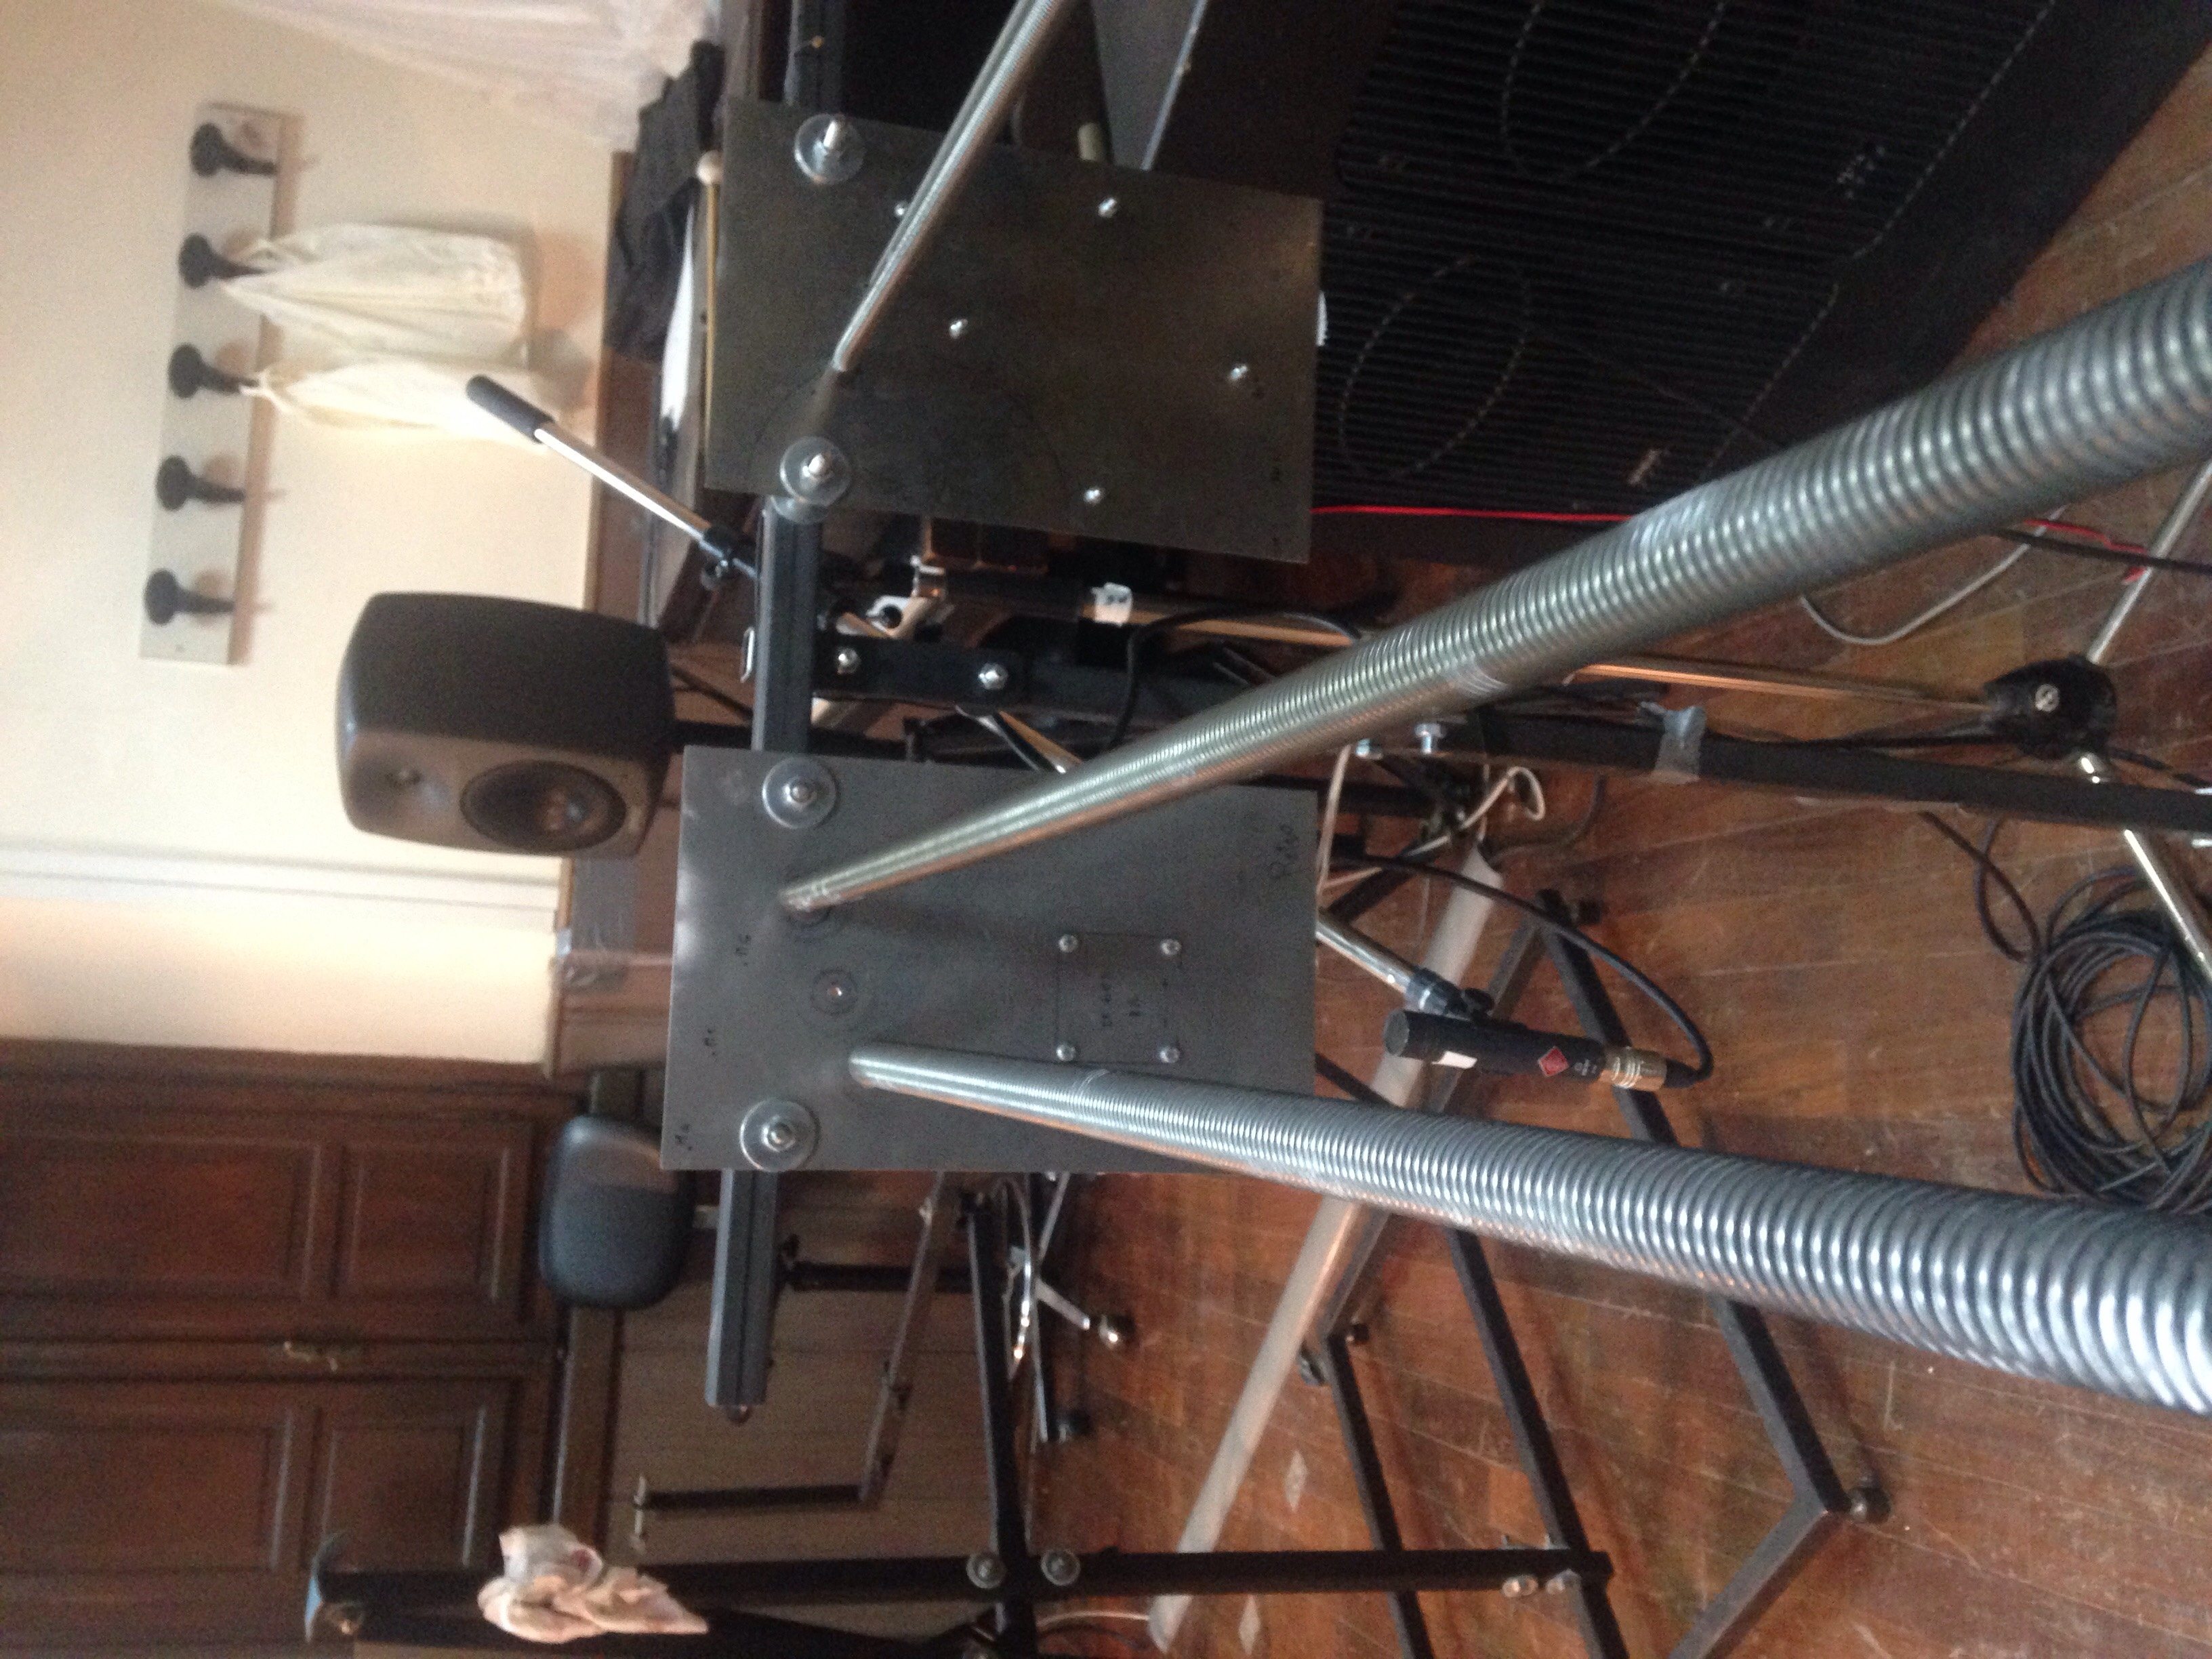
\includegraphics[height=6cm, width=5cm, angle=0,
%          keepaspectratio]{Spire2.jpg}
%\end{figure}

Tutti gli studi sono stati fatti su acciaio armonico o acciaio inox. Due sono i fattori che regolano il funzionamento della molla a trazione:

\begin{enumerate}
\item{Diametro del filo}
\item{Larghezza del diametro esterno (\textit{spira})}
\end{enumerate}

Il diametro del filo (1.) unito alla larghezza del diametro esterno (2.) rendono possibile il cambiamento della qualità della flessione della molla. Anche il numero di spire agisce sulla flessione della molla.

%************************************************

\clearpage

\section{Fissaggio Molle e attuatori}

Un basamento unisce quattro placche di metallo che montano tre molle ciascuna, tese per la lunghezza paritaria di 80 centimetri. Il basamento è in ferro, le placche rettangolari, in acciaio armonico, le molle in ferro armonico. Nel primissimo prototipo una delle molle, la numero 4\footnote{guardare la \textit{Legenda} sita in partitura} era in acciaio inox, ma non avendo ottenuto i risultati acustici sperati, ho deciso di cambiarla. 

\begin{figure}[htbp]
\begin{center}
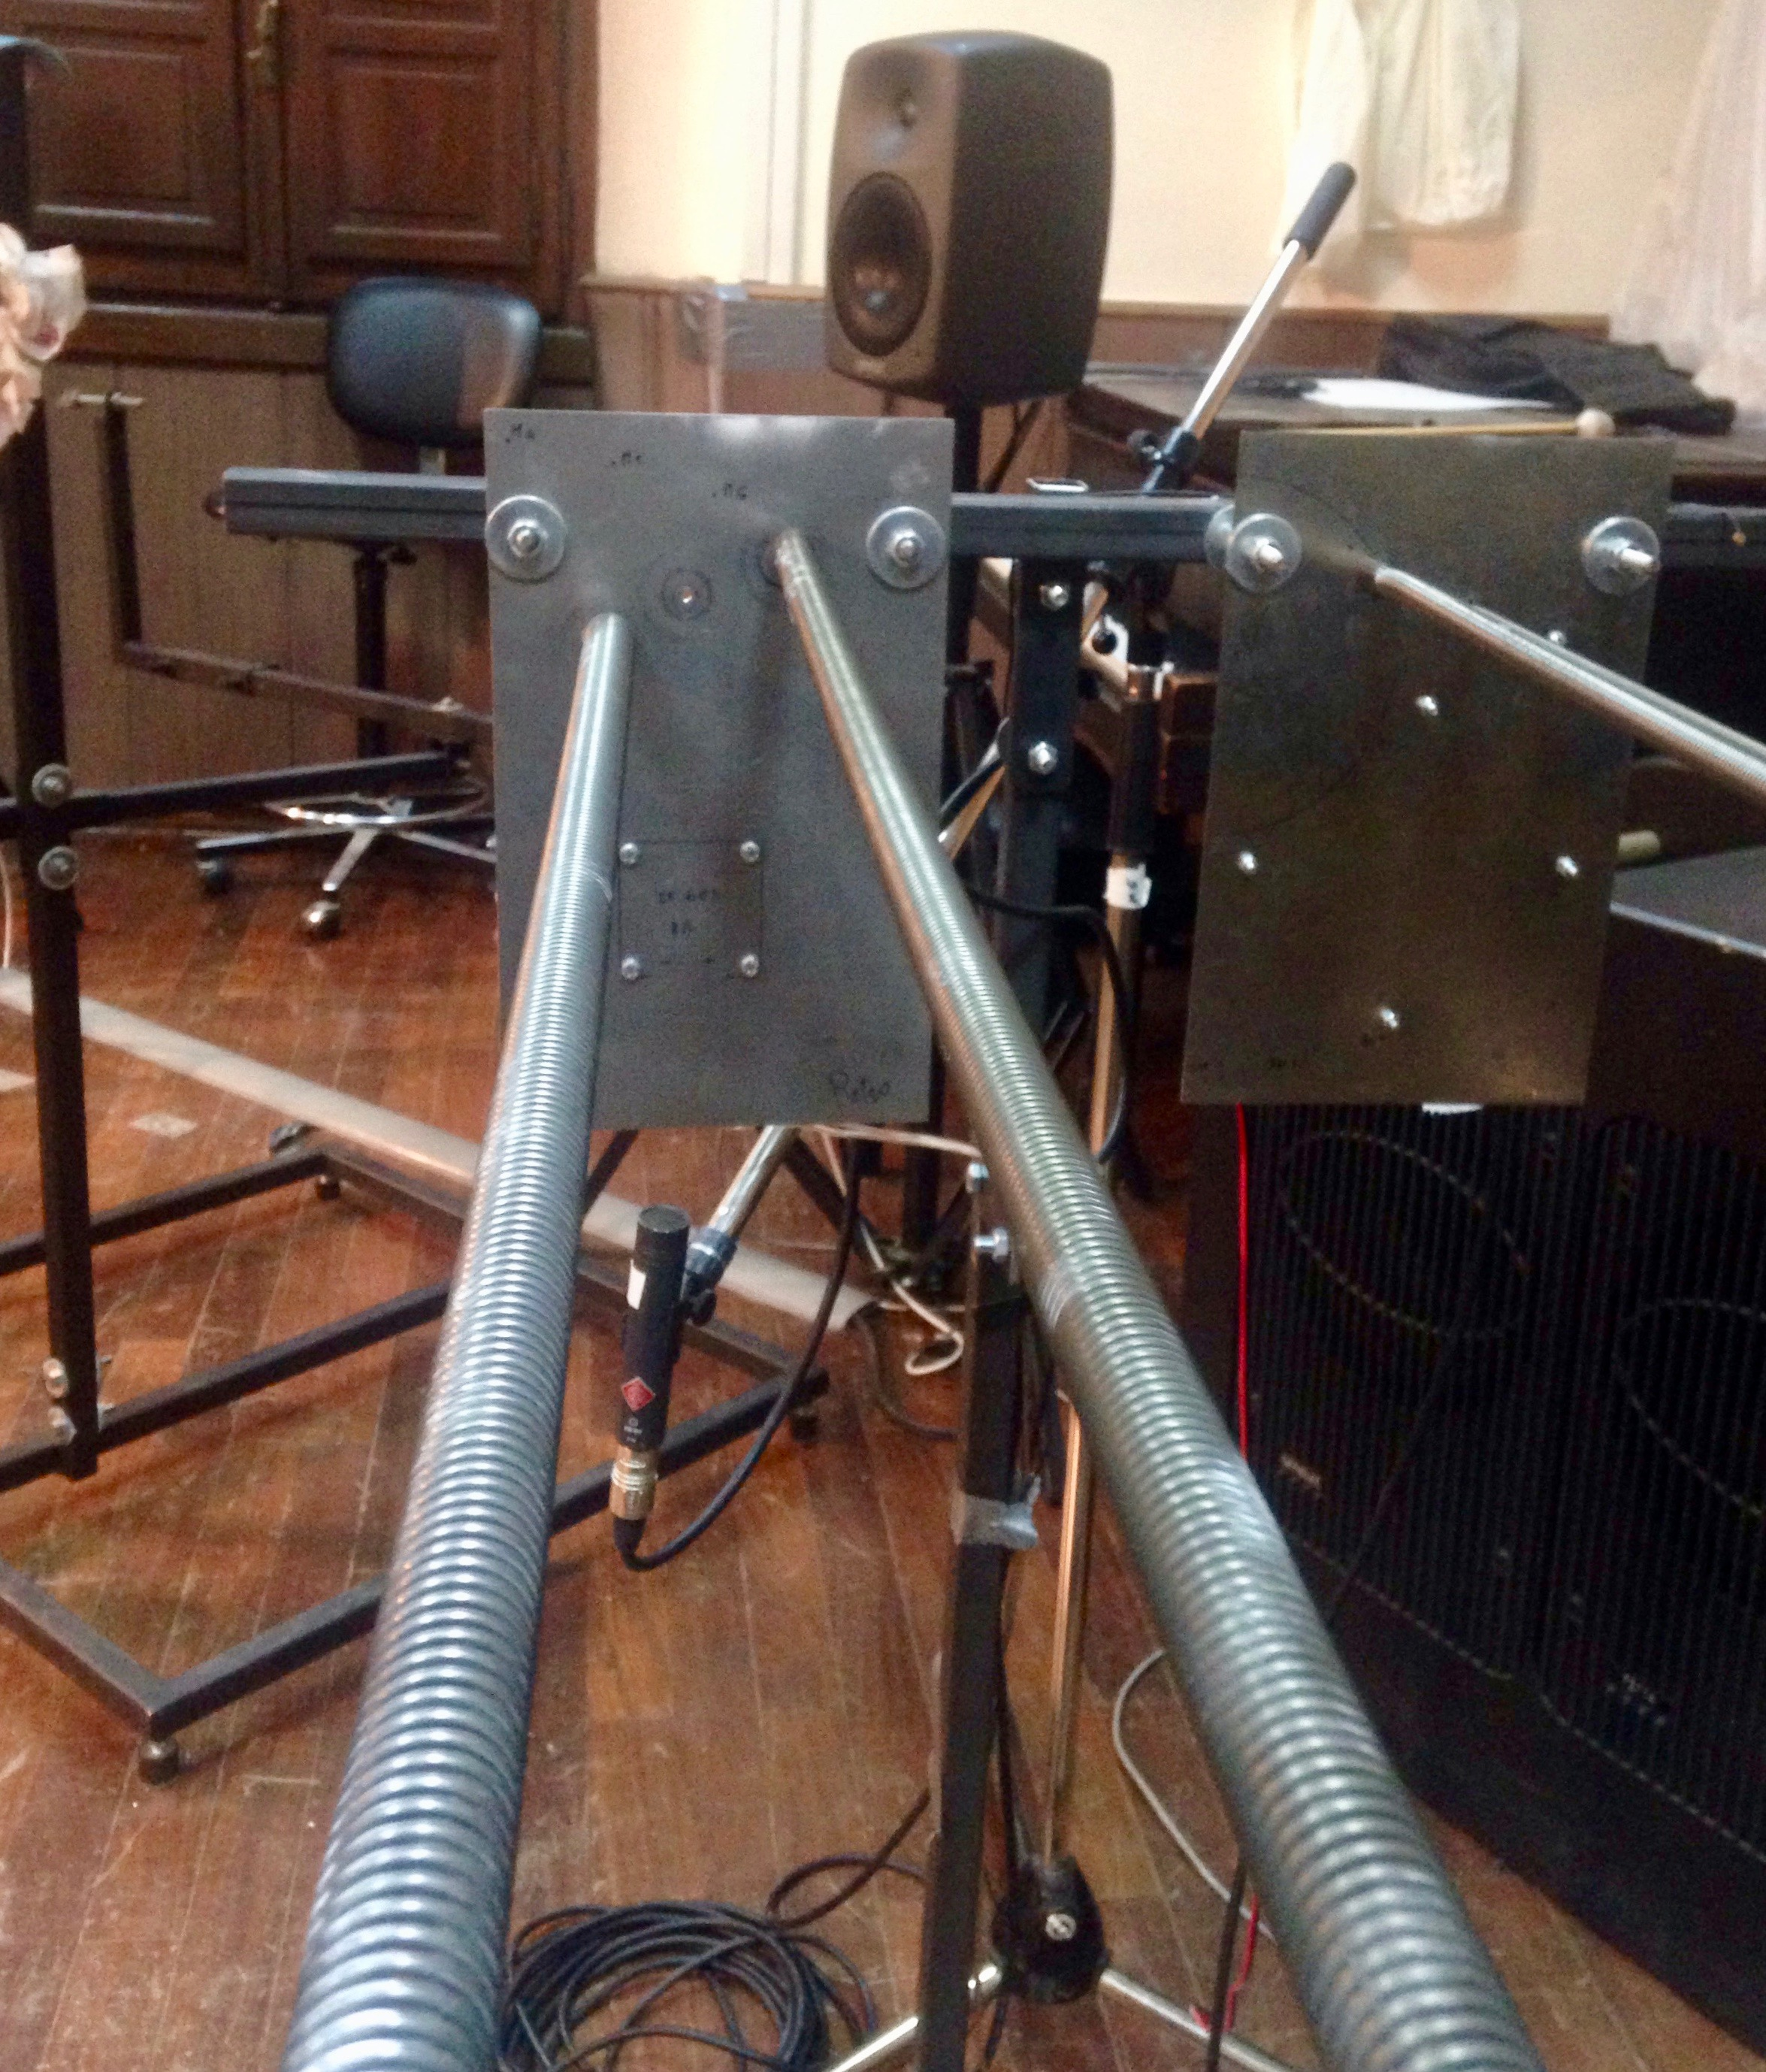
\includegraphics[width=.99\textwidth]{Spire2cc.jpg}
\caption{\textit{Sp.I.R.E.}, particolare della sezione più grave (Molla 5-4)}
\label{default}
\end{center}
\end{figure}

Le molle sono disposte sulle placche in due sezioni a gradini (\textit{fig. 13}) come se si andasse a suonare un violoncello, o un contrabbasso in posizione orizzontale. Durante la creazione di questo primo prototipo ho voluto utilizzare solo cinque molle per un'esigenza timbrica: alcune molle di diametro maggiore a scontrarsi, altre di diametro simile avevano la stessa risultante timbrica. 

\begin{figure}[t]
\begin{center}
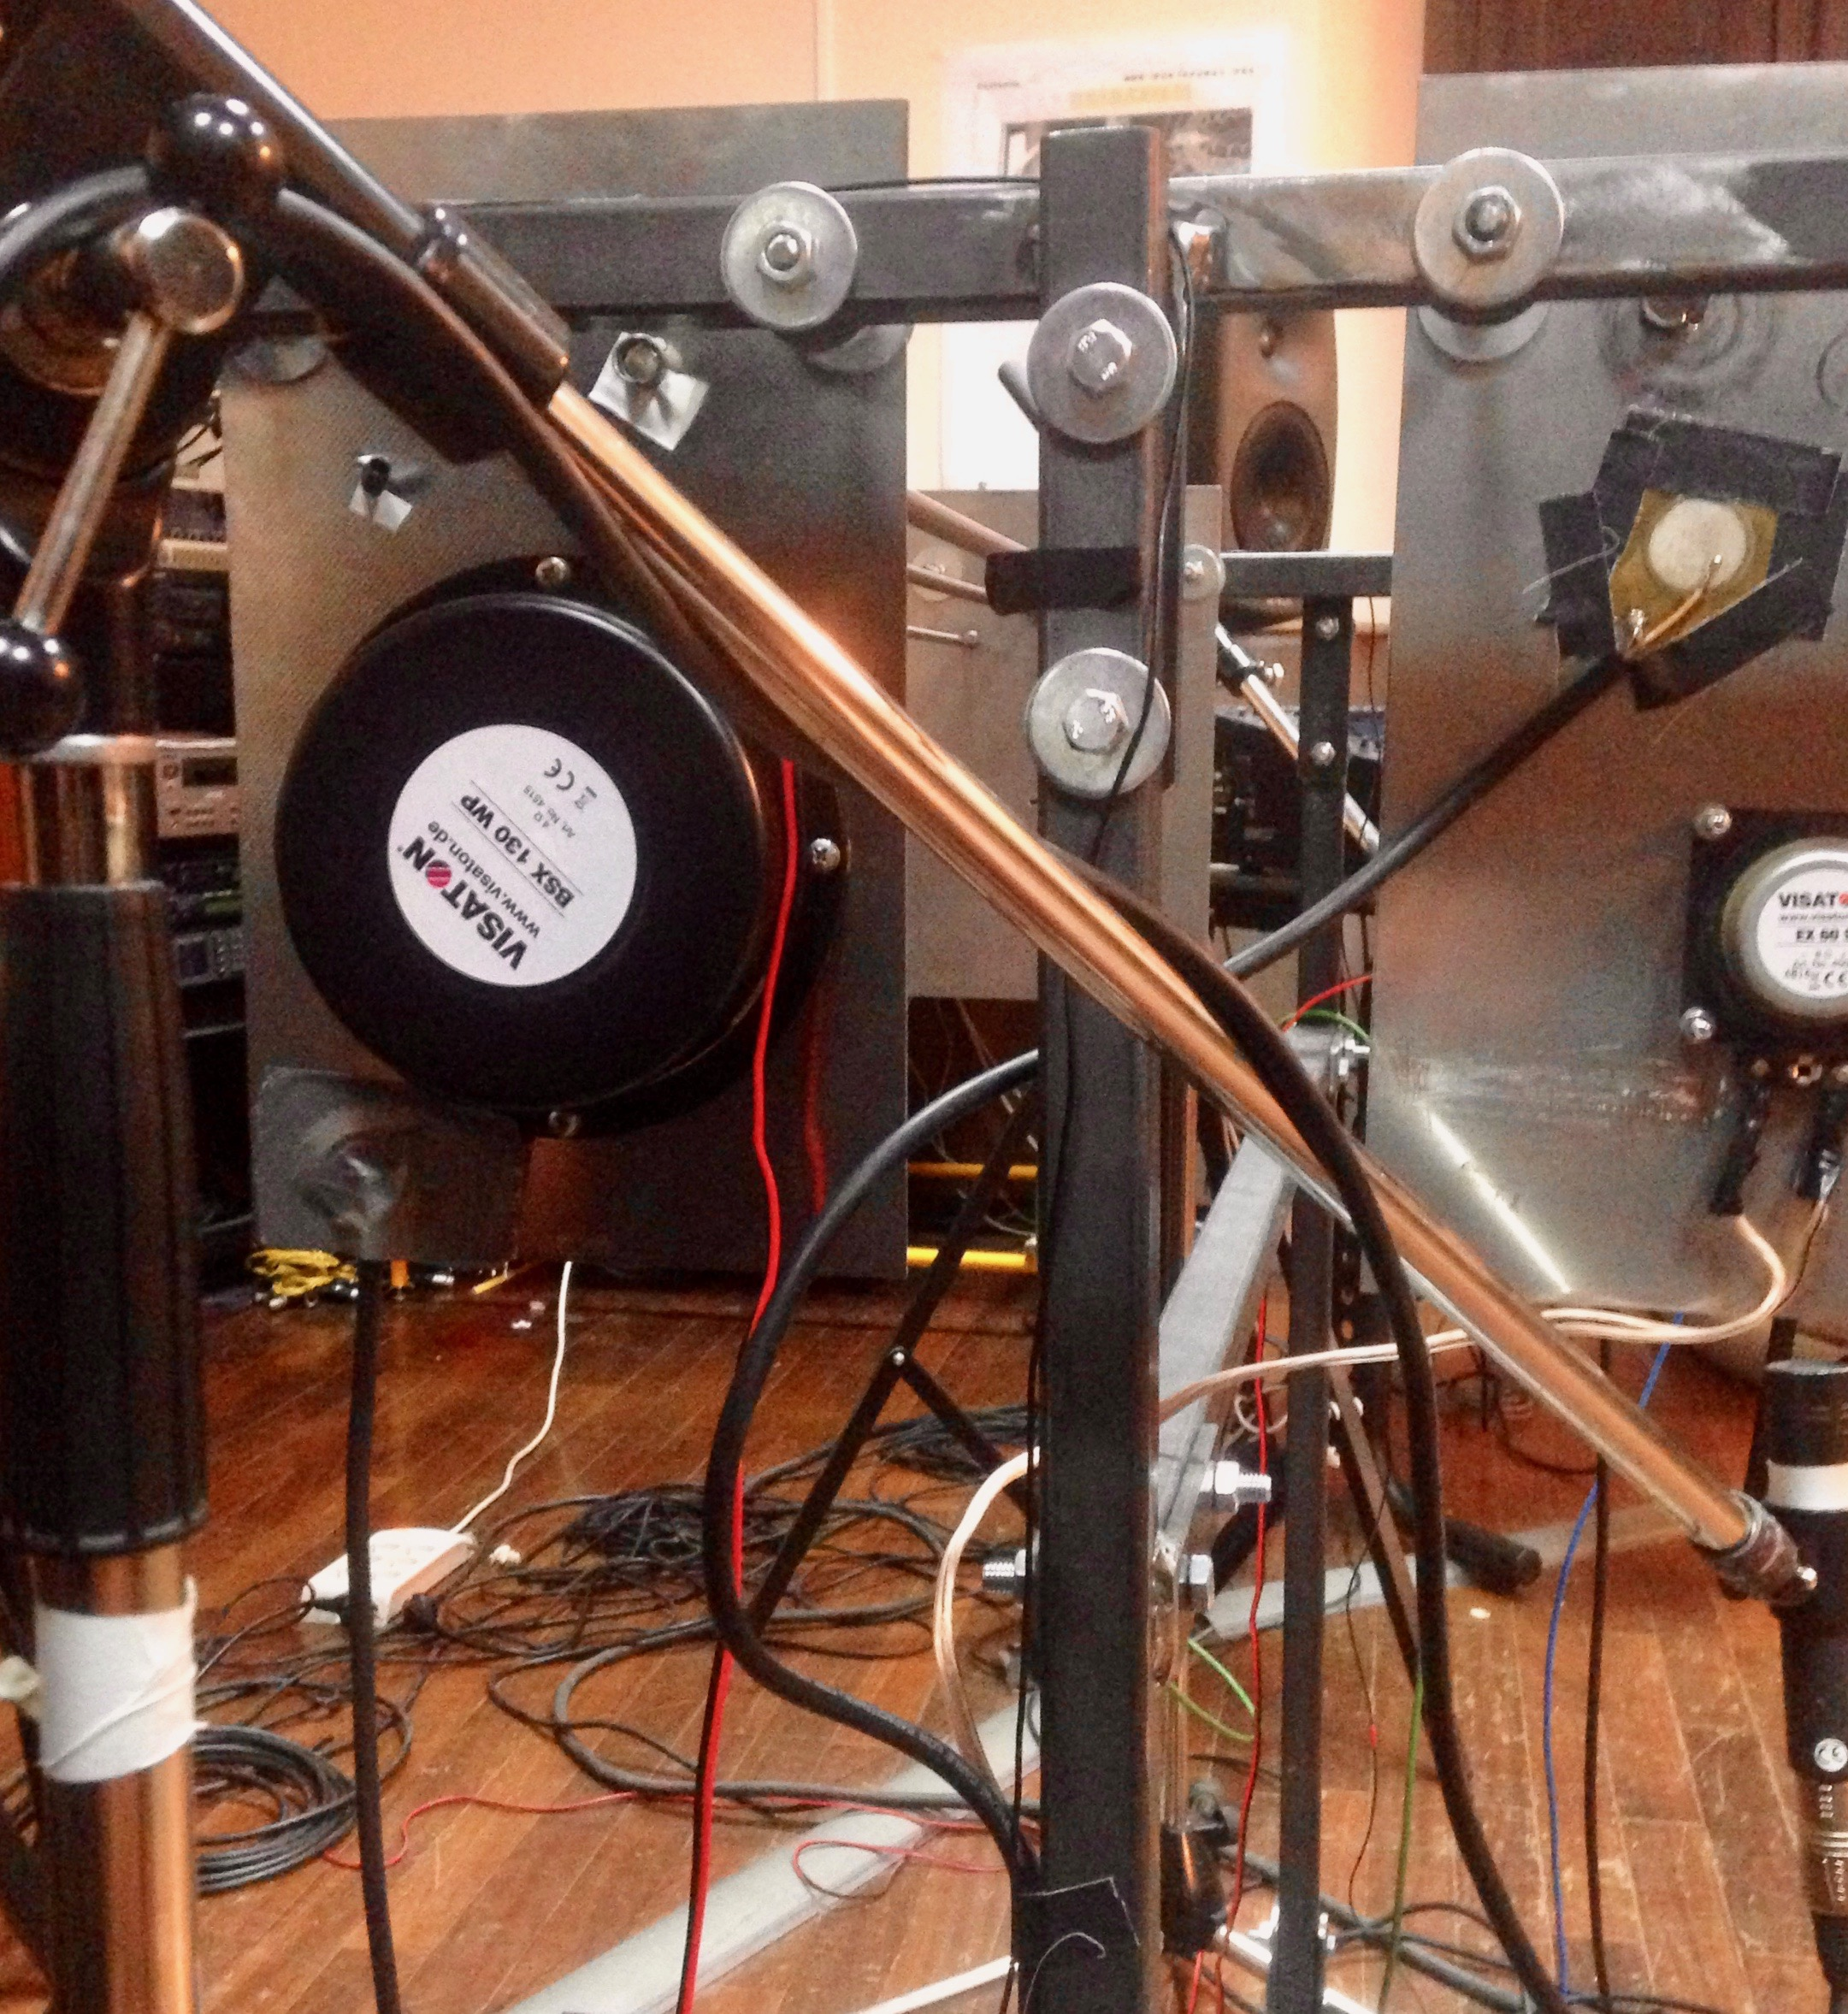
\includegraphics[width=.99\textwidth]{Spire1cc.jpg}
\caption{particolare attuatori BSX e ESX60}
\label{default}
\end{center}
\end{figure}

Gli attuatori sono stati fissati preventivamente tramite del nastro su una delle piastre di metallo e fatte delle prove di risposta del materiale risuonante. Trovato eccellente la risposta del metallo, in questo caso ferro e ferro zigrinato, sono stati segnati dei punti di ancoraggio degli attuatori, tramite viti con rondelle e bulloni.

\clearpage 

\begin{tabularx}{\textwidth}{Xccc}
\toprule
\textbf{Tipologia} & \textbf{ATTACCO} & \textbf{BATTENTE} & \textbf{Risposta} \\
\midrule \textbf{METALLI} & & & \\
\midrule 
Placche metallo & 8 Risonatori & Ottima \\
\midrule 
Molle a trazione Inox & 2 & Strumento & Sufficiente \\
\midrule 
Molle a trazione Acciaio armonico & 6 & Strumento & Ottima\\
\midrule 
Tubo Quadrato Ferro & 2 & Basamento & Ottima\\
\midrule 
Viti per innesti & Varie & Bas. Attuatori & Ottima\\
\midrule 
\textbf{MOLLE}\\
\midrule 
BSX 130 WP - 4 Ohm & 4 & Vibrazione Placca & Ottima\\
\midrule 
ESX 45 - 8 Ohm & 4 & Vibrazione Placca & Sufficiente\\
\midrule 
ESX 60 - 8 Ohm & 3 & Vibrazione Placca & Buona\\
\midrule 
\textbf{MAGNETI}\\
\midrule 
Humbucker & 2 & Amplificazione Molle & Buona\\
\midrule 
Double Coil Bass & 1 & Amplificazione Molle & Ottima\\
\midrule 
\textbf{PIEZOELETTRICI} \\
\midrule 
Piezoelettrici & 4 & Amplificazione Molle & Buona\\
\bottomrule
\end{tabularx}

\clearpage

%************************************************

\section{Schema Elettrico}
Di seguito, lo schema elettrico per il collegamento degli attuatori:

\begin{figure}[htbp]
\begin{center}
\includegraphics[width=.99\textwidth]{Elettrico.jpg}
\caption{Lo schema elettrico per il collegamento degli attuatori}
\label{default}
\end{center}
\end{figure}


% !TEX TS-program = pdflatex
% !TEX encoding = UTF-8 Unicode

%************************************************
\chapter{Sistema di diffusione}
\label{chp:Sistema di diffusione}
%************************************************

\epigraph{Come un rosone nel cuore di un tempio immenso}{\textit{Antonin Artaud}}

La diffusione sonora di Vitres de Son è basata sull'utilizzo di 9 dei 22 altoparlanti (più il sub-woofer) presenti nella cupola sonora "Il suono di Piero" costruita nel all'interno dell'Aula I del III piano del conservatorio Santa Cecilia. \begin{figure}[!htbp]
\begin{center}
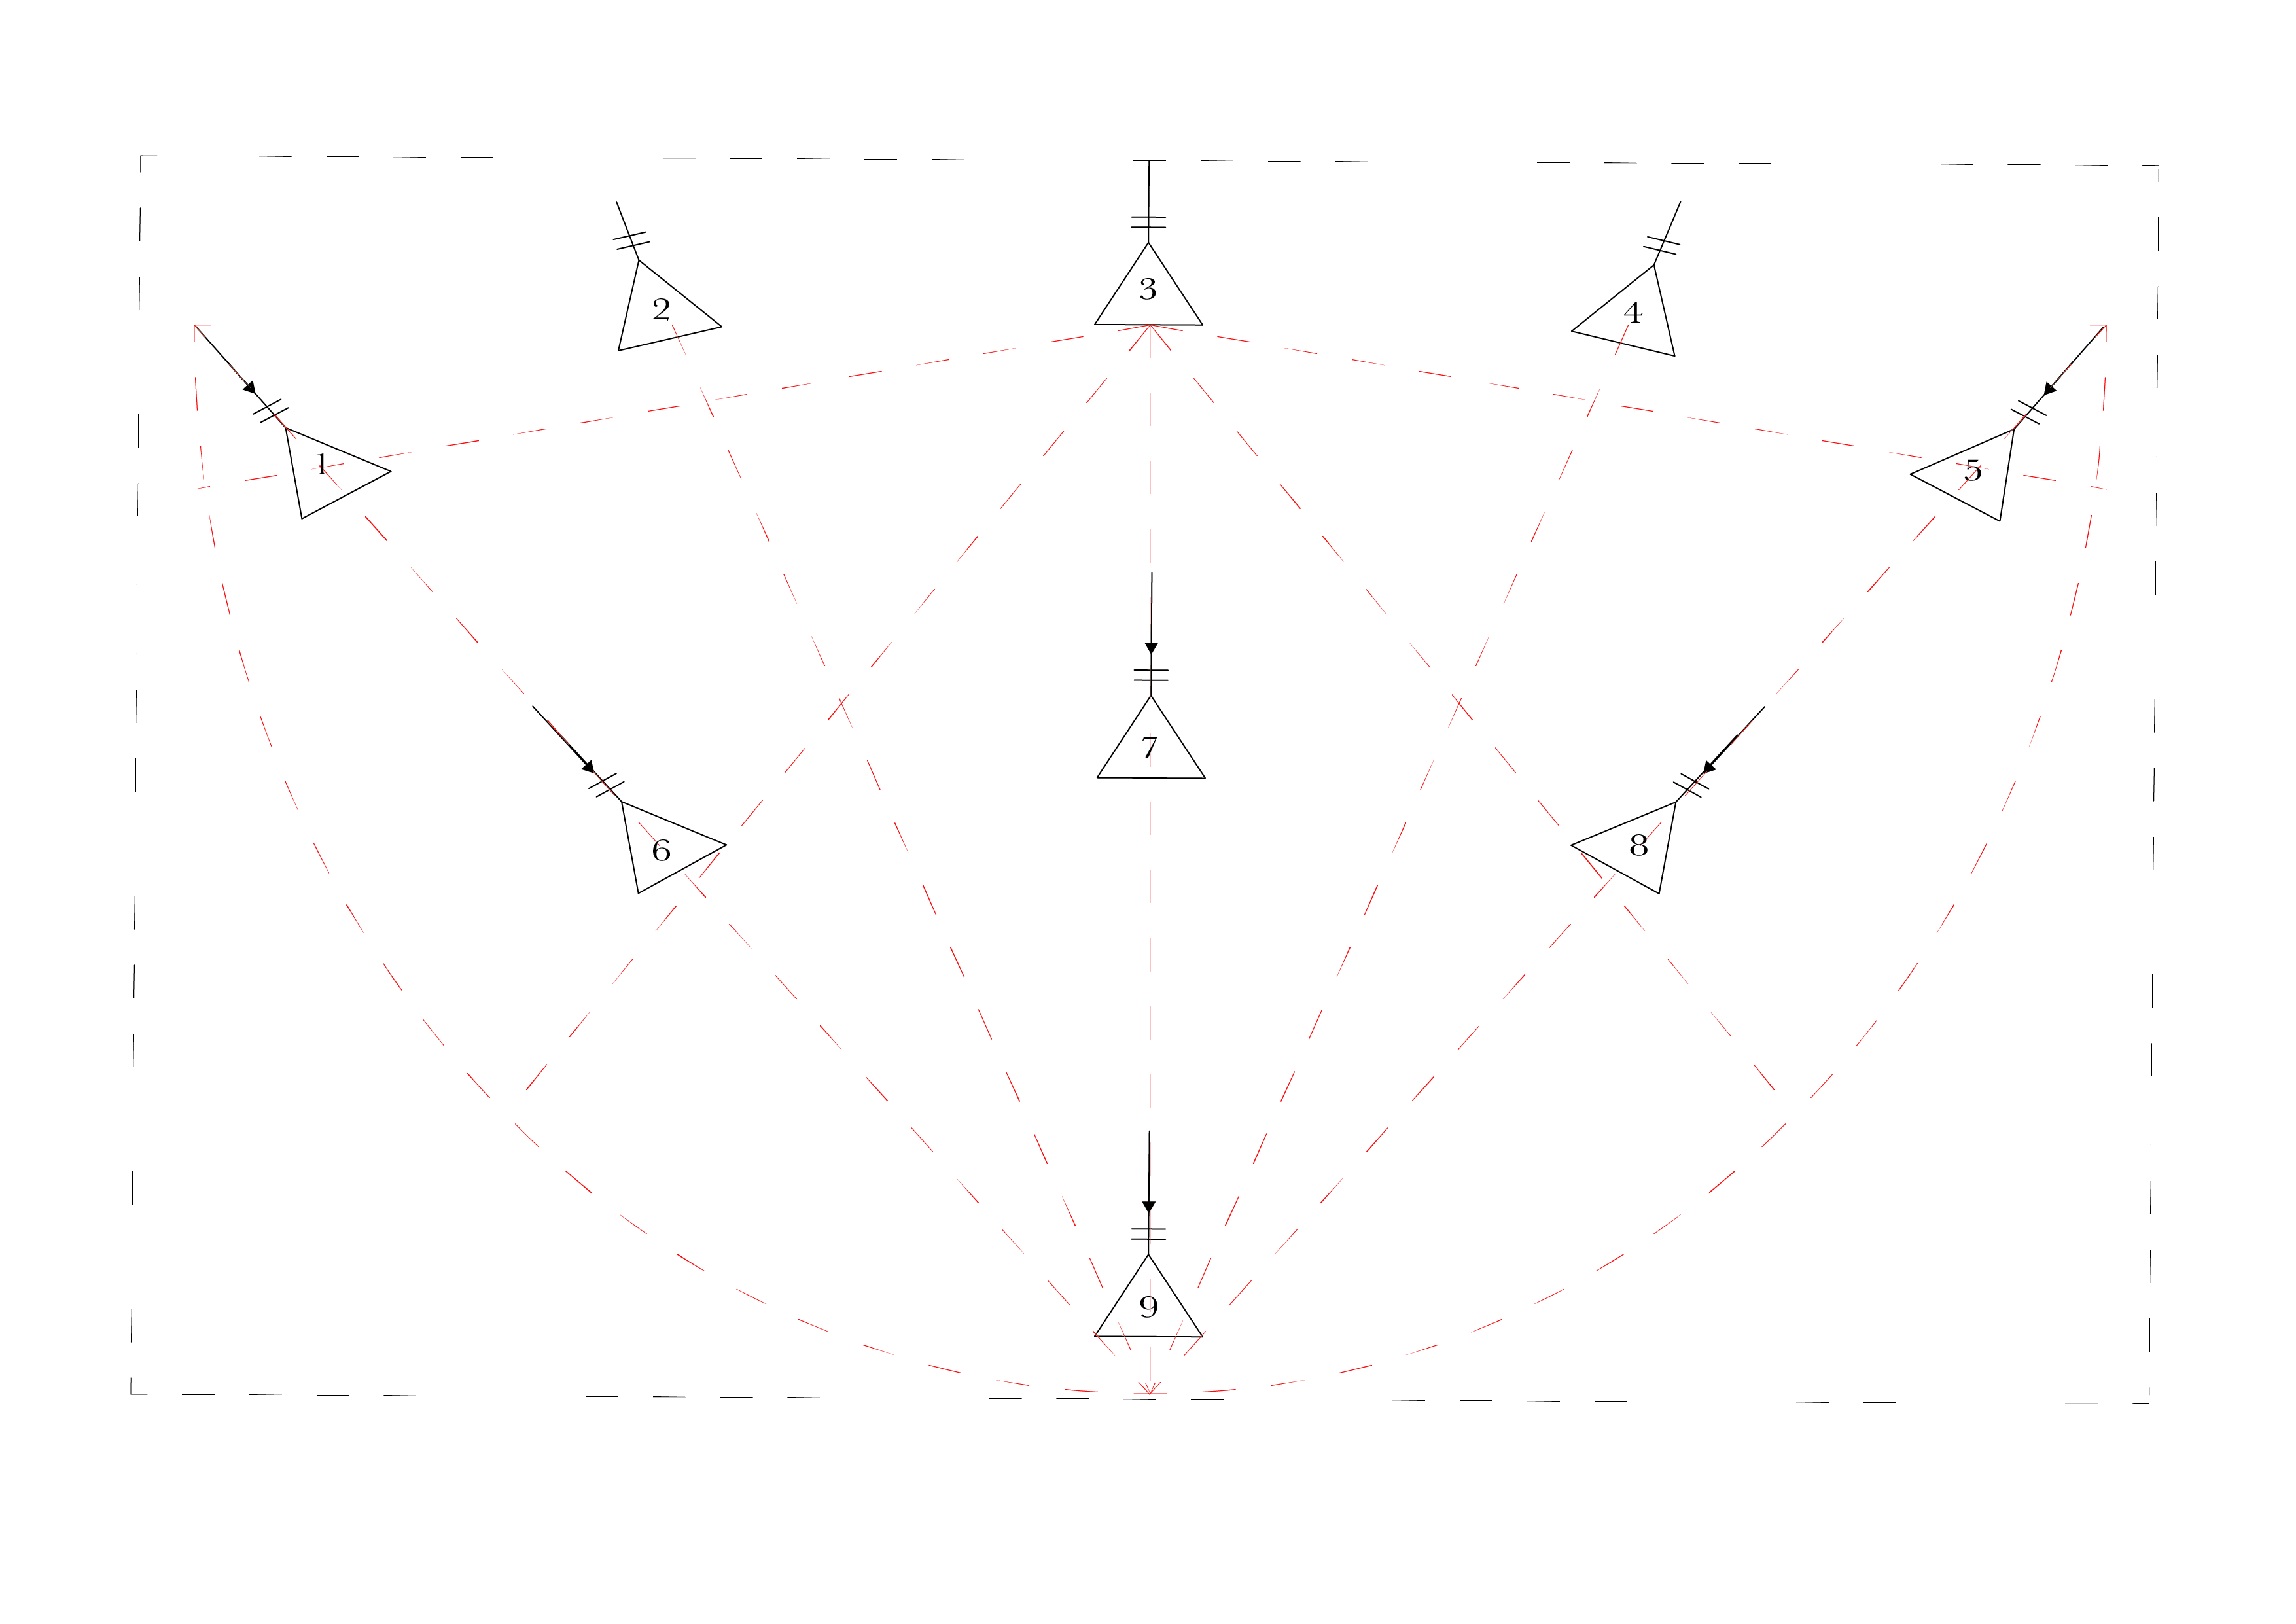
\includegraphics[width=1\textwidth]{legenda02.png}
\caption{Diffusione a \textit{A Rosone} di Vitres de Son}
\label{default}
\end{center}
\end{figure}Sfruttare solo una parte della cupola è legato alle mie esigenze composizione, sia a livello di figura nella quale far adagiare l'esecutore che lo Sp.I.R.E.. Come rappresentato nella figura qui sopra, notiamo che i diffusori più esterni sono i vertici di un triangolo inscritto in un arco: significante dell'immagine del rosone. Il suono confluisce al centro e la microfonazione ci dà la possibilità di apprezzarlo nei suoi spostamenti. Sottolineo, inoltre, che la spazializzazione è data esclusivamente dall'amplificazione trasparente.
Per la costruzione del sistema di diffusione ho utilizzo gli scritti introduttivi che sono allegati a molte partiture di Luigi Nono e Karlheinz Stockhausen (che verranno svelate in seguito). Il compositore non è più slegato da una realtà percettiva e teatrale del produzione sonora, ma diventa artefice della disposizione degli altoparlanti e del pubblico all'interno dell'ambiente d'ascolto.
Vediamo nel dettaglio il sistema di ripresa e la diffusione audio che da partitura diventano parte integrante della composizione.

\section{Sistema di ripresa}
La diffusione audio avverrà tramite l'utilizzo di un sistema di ripresa omnidirezionale che renderà possibile la diffusione omogenea del materiale acustico ed elettronico prodotto da Sp.i.r.e..
\begin{figure}[!htbp]
\begin{center}
\includegraphics[width=.99\textwidth]{ripresa.jpg}
\caption{Ripresa microfonica dello Sp.I.R.E.}
\label{default}
\end{center}
\end{figure}
Di seguito, i materiali tecnici da utilizzare per la riproduzione dell'opera:
\begin{itemize}
	\item{Scheda Audio 8in 9out}
	\item{Mixer Yamaha DM1000}
	\item{4 piezoelettrici}
	\item{2 microfoni dpa omnidirezionali}
	\item{2 microfoni Cardioide Neumann}
	\item{Cablaggio}
	\item{1 Amplificatore di potenza da 4 canali a 4 Ohm}
	\item{Computer\\}
\end{itemize}

\section{Diffusione} 

Per schematizzare e disegnare la diffusione audio, ho utilizzato come esempio gli scritti introduttivi e le legende di due partiture contemporanee. Specificatamente: \textit{Mantra} di Karlheinz Stockhausen e \textit{Prometeo, Tragedia dell'ascolto} di Luigi Nono. Nella partitura di Stockhausen \begin{figure}[!htbp]
\begin{center}
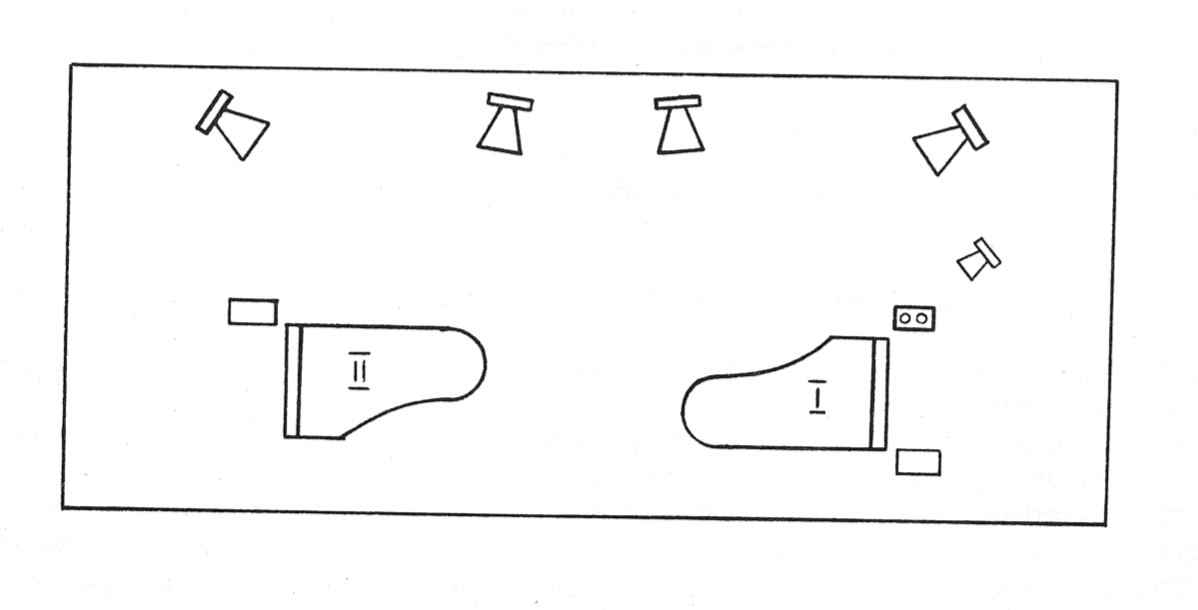
\includegraphics[width=.99\textwidth]{Mantra.jpg}
\caption{Particolare della Legenda di \textit{Mantra}}
\label{default}
\end{center}
\end{figure}
vediamo come il compositore esplica lucidamente il rapporto che c'è tra diffusione ed elaborazione del segnale, in un solo schema racchiude sia la diffusione che l'elaborazione.\begin{figure}[htbp]
Nono, nel Prometeo, aggiunge agli schemi algoritmici e di diffusione, anche la disposizione del pubblico in sala. Questa è un passo importante per la storia della musica elettroacustica, perché alla modalità d'ascolto si aggiunge un fattore importante per la stesura di un lavoro compositivo: la regia. Nono era sempre attento al rapporto fra diffusione del suono e disposizione dell'ascoltatore.
Prendendo ad esempio i maestri, ho lavorato su un'irradiazione tale da poter favorire un spostamento del suono a livello spaziale. La tipologia di microfonazione e la disposizione dei diffusori, permette:
\begin{center}
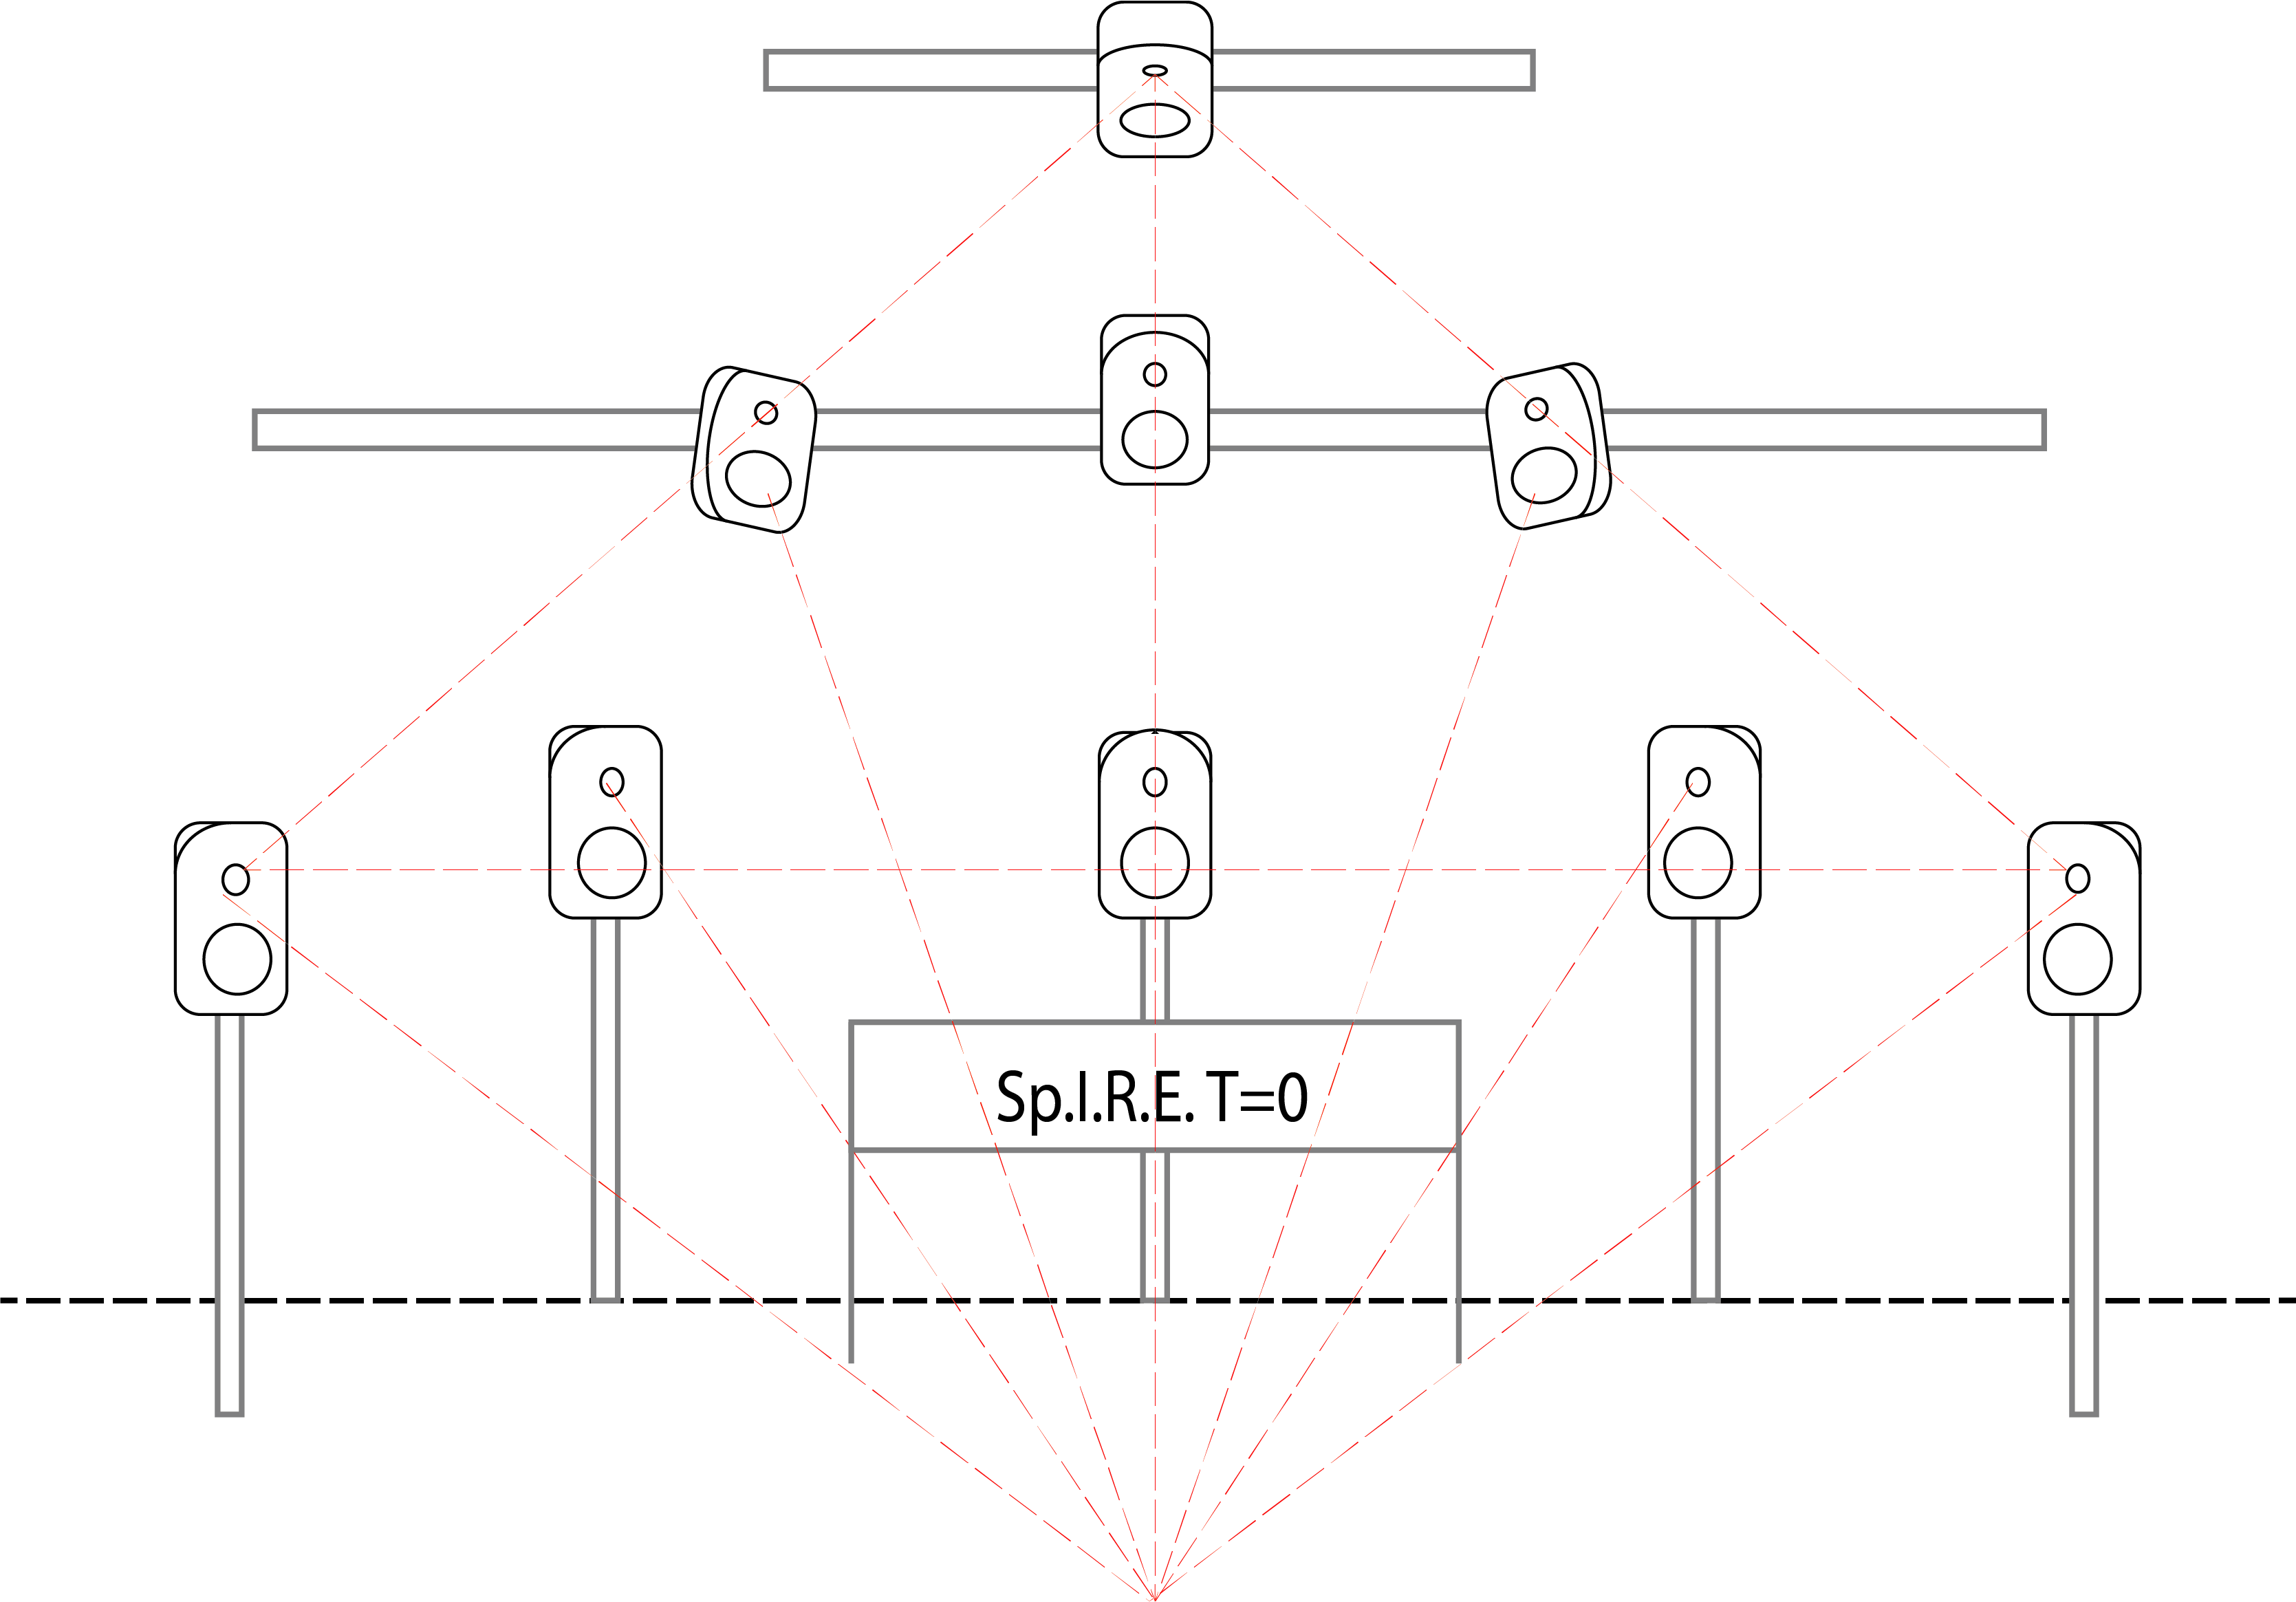
\includegraphics[width=.99\textwidth]{diffusione.png}
\caption{Diffusione a \textit{A Rosone} di Vitres de Son. \textit{Prospettiva}}
\label{default}
\end{center}
\end{figure}

\begin{itemize}
\item{La disposizione dei microfoni (figura 20) rende possibile un movimento spaziale del segnale. Sicuramente anche la scrittura ho tenuto conto di questo effetto, scrivendo gesti puntuali quando ritenevo strutturale uno spostamento della fonte sonora nello spazio.}
\item{La serie di filtri presente a valle, prima della diffusione, permette un movimento del suono verso l'alto, dato anche dall'utilizzo di diffusori sospesi al di sopra dello strumento}
\end{itemize}

L'amplificazione trasparente ed il filtraggio danno corporeità al suono e oltre a rendere possibile una spazializzazione realistica dello strumento, si da anche la possibilità alla stanza di risuonare su determinate frequenze dato il lungo decadimento dello Sp.I.R.E..


% !TEX TS-program = pdflatex
% !TEX encoding = UTF-8 Unicode
% !TEX root = ../ArsClassica.tex

%************************************************
\chapter{Riflessioni e conclusioni}
\label{chp:Riflessioni e conclusioni}
%************************************************

La strada percorsa fino a questo momento non delinea la fine di un percorso, ma bensì uno step. Un varco importante verso una determinata considerazione degli eventi musicali e dell'evoluzioni del suono.
La strada percorsa fino ad ora non arriva a delineare la fine di un percorso, ma piuttosto un inizio. \\
Questo lavoro di tesi lo identifico di più come un percorso costruito su un ponte che ancora sto attraversando che mi spinge sempre più verso una consapevolezza artistica. Tale consapevolezza rende giorno per giorno meno vacillanti le fondamenta di questo ponte di transito verso una maturità stilistica: è la drammaturgia di una struttura musicale in divenire. \\
L'idea che ogni frase, sia ritmica che melodica, risulto come un entità a sé è il passo odierno e sul quale voglio continuare le mie ricerche formali. Ogni modifica, ogni variazione, è legata ad un determinato personaggio musicale, che si modifica nell'aspetto e nella forma durante ogni cambiamento di oggetti/esseri limitrofi. \\
Anche a livello compositivo cercherò di esprimere tale costrutto: l'identità di ogni struttura dovrà essere ben salda ed ogni suo mutamento risultare pieno di un proprio significato espressivo, colmo di quella trasformazione intrinseca alle modifiche sul materiale sonoro. Vorrei che il mio studio compositivo futuro sia un lungo viaggio: verso la conoscenza di altre identità in trasformazione che incontrerò lungo le strade e i percorsi che purtroppo o per fortuna la vita ci propina, sempre con la speranza di una nascita nella quale si veda il sole.



% !TEX TS-program = pdflatex
% !TEX encoding = UTF-8 Unicode
% !TEX root = ../2018-03-26-papa-vitres-de-son.tex

%************************************************
\chapter{Bibliografia}
\label{chp:Bibliografia}
%************************************************

Antonin Artaud, \textit{Poesie della crudeltà} (a cura di P. Di Palmo), Stampa alternativa, Roma, 2002. \\
Pubblicata per la prima volta nel 1925 \\
\\
Antonin Artaud, \textit{Il teatro e il suo doppio}, Einaudi Autore, Roma, 1968 \\
\\
Walter Branchi, \textit{Tecnologia della musica elettronica} (con prefazione di Domenico Guaccero), Lerici, Roma, 1977 \\
\\
John Cage, \textit{Confessioni di un compositore} in AA.VV. (a cura di G. Bonomo e G. Furghieri), \textit{Riga n. 15} - John Cage, Milano, Marcos y Marcos, Milano, 1998\\ 
\\
Sergio Cingolani e Renato Spagnolo, \textit{Acustica musicale e architettonica}, UTET, Torino, 2004 \\
\\
Guido Facchin,  \textit{Le percussioni}, EDT, 2000 \\
\\
Samuel Z. Solomon, \textit{How to Write for Percussion: A Comprehensive Guide to Percussion Composition},  
Oxford University Press, Gran Britannia, 2016\\
 \\
James Holland, \textit{Practical Percussion: A Guide to the Instruments and Their Sources}, 2005 \\
\\
Curtis Roads, \textit{Composing electronic music, A New Aesthetic} OUP USA, 2015 \\
\\
Curtis Roads, \textit{The Computer music tutorial}, 1996 \\
\\
Tanja Orning \textit{Pression} (a performance study) Norwegian Academy of MusicMusic Performance Research Copyright © 2012 Royal Northern College of Music Vol. 5
\\
Iannis Xenakis, \textit{Universi del suono, Scritti e interventi 1955-1994} (a cura di Agostino Di Scipio), Ricordi S.r.l. e LIM Editrice S.r.l., 2003 \\
\\
Zaffiri Enore, \textit{Due scuole di musica elettronica in Italia} Silva Editore, Milano, 1968 

% !TEX TS-program = pdflatex
% !TEX encoding = UTF-8 Unicode

%************************************************
\chapter{Partiture}
\label{chp:Partiture}
%************************************************

Karlheinz Stockhausen, \textit{Mantra}

Helmut Lachenmann, \textit{Pression}

Pierre Jodlowski, \textit{Ombra della mente}

Domenico Guaccero, \textit{Variazioni II}

Luigi Nono, \textit{Prometeus}

Luigi Nono, \textit{Polifonia, monodia, ritmica}

Luigi Nono, \textit{Post Prae-Ludium per Donau}

Simone Santi Gubini, \textit{Klangrelief (Relief II)}


\clearpage

% !TEX TS-program = pdflatex
% !TEX root = ../ArsClassica.tex

%*******************************************************
% Bibliography
%*******************************************************
\nocite{*}
\printbibliography

%!TEX TS-program = pdflatex
%!TEX encoding = UTF-8 Unicode
%!TEX root = ../2018-03-26-papa-vitres-de-son.tex

%*******************************************************
% Introduzione
%*******************************************************
\chapter*{Ringraziamenti}

\pdfbookmark{Ringraziamenti}{Ringraziamenti}

\textit{I più vivi ringraziamenti a tutti i colleghi ed i maestri della} \textbf{Scuola di musica elettronica} \textit{del Conservatorio di Santa Cecilia \\ che mi hanno supportato (e sopportato), durante la stesura della tesi e del lavoro di ricerca.}
\\
\\
\textit{Ringrazio il CRM per il grande aiuto morale e fisico che mi ha dato per la creazione di Sp.I.R.E.}
\\
\\
\textit{Ringrazio Matteo, per la pazienza}

\end{document}
